\documentclass[tombow,dvipdfmx]{corona-a5-1.1}
% dvipdfmxを追加(川口)

% Springer document settings
\usepackage[bottom]{footmisc}% places footnotes at page bottom

\usepackage{newtxtext}       % 
\usepackage[varvw]{newtxmath}       % selects Times Roman as basic font
%%%%%%%%%%%%%%%%%%%%%%%%%%%%%%%

% \usepackage{amssymb}
\usepackage{ntheorem}
\usepackage{amsmath}
\usepackage{enumitem}


\usepackage{graphicx}
\usepackage{color}
\usepackage{cite}
\usepackage{makeidx}


\usepackage{ascmac}
\usepackage{eclbkbox}
\usepackage{dsfont}

\usepackage{longtable}

\usepackage{url}

\usepackage{hyperref}

\usepackage{multicol}

%% --川口追加--
\makeatletter
\let\MYcaption\@makecaption
\makeatother
\usepackage{subcaption}
\captionsetup{compatibility=false}      % 必要に応じて

\makeatletter
\let\@makecaption\MYcaption
\makeatother
% ----

%%
\theoremstyle{plain}
\theoremheaderfont{\bfseries}
\theorembodyfont{\rmfamily}
\theoremseparator{\hspace{1ex}}
\theoremindent0cm
\theoremnumbering{arabic}
\theoremprework{\vspace{1ex}\begin{shadebox}\vspace{1ex}}
\theorempostwork{\vspace{-1ex}\end{shadebox}\vspace{1ex}}

%%
\theoremclass{theorem}

%%
\theoremclass{theorem}

%%
\theoremclass{theorem}


%%
\theoremstyle{break}
\theoremheaderfont{\bfseries}
\theorembodyfont{\rmfamily}
\theoremseparator{}
\theoremindent0cm
\theoremnumbering{arabic}
\theoremprework{\vspace{1.5ex}\begin{breakbox}\vspace{-0.5ex}}
\theorempostwork{\vspace{-0.5ex}\end{breakbox}\vspace{1.5ex}}

%%
\theoremstyle{nonumberplain}
\theoremseparator{\hspace{1ex}}

%%
\newtheorem{assumption}{Assumption}[section]

%%
\renewcommand{\theproblem}{}

\renewcommand{\theremark}{}


\newcommand{\red}[1]{{\color{red}#1}}
\newcommand{\blue}[1]{{\color{blue}#1}}
\newcommand{\green}[1]{{\color{green}#1}}

\DeclareMathOperator*{\argmax}{arg\,max}

\newcommand{\bm}[1]{\boldsymbol{#1}}
\newcommand{\sfT}{\mathsf{T}}

\newcommand{\advanced}{$^{\ddag}$}

\DeclareMathOperator{\sfsin}{\mathsf{sin}}
\DeclareMathOperator{\sfcos}{\mathsf{cos}}
\DeclareMathOperator{\sftan}{\mathsf{tan}}
\DeclareMathOperator{\sfarctan}{\mathsf{arctan}}

\DeclareMathOperator{\sfdiag}{\mathsf{diag}}
\DeclareMathOperator{\sfcol}{\mathsf{col}}
\DeclareMathOperator{\sfdet}{\mathsf{det}}
\DeclareMathOperator{\sfadj}{\mathsf{adj}}
\DeclareMathOperator{\sftrace}{\mathsf{trace}}

\DeclareMathOperator{\real}{\mathsf{Re}}

\DeclareMathOperator{\sfker}{\mathsf{ker}}
\DeclareMathOperator{\sfim}{\mathsf{im}}

\DeclareMathOperator{\sfdim}{\mathsf{dim}}
\DeclareMathOperator{\sfspan}{\mathsf{span}}

\DeclareMathOperator{\sfint}{\mathsf{int}}

\DeclareMathOperator*{\sfmin}{\mathsf{min}}
\DeclareMathOperator*{\sfmax}{\mathsf{max}}
\DeclareMathOperator*{\sfsup}{\mathsf{sup}}

\DeclareMathOperator{\sfsat}{\mathsf{sat}}

\newcommand{\mat}[1]{\left[\: \begin{matrix} #1 \end{matrix} \:\right]}
\newcommand{\spliteq}[1]{\begin{split} #1 \end{split}}
\newcommand{\simode}[1]{\begin{cases}  \begin{split} #1 \end{split} \end{cases}}

\newcommand{\proofend}{\hfill \rule{2mm}{3mm}}

\newcommand{\Xti}{X_i'}
\newcommand{\Xsi}{X_i}

\newcommand{\Xtone}{X_1'}
\newcommand{\XtN}{X_N'}

\newcommand{\Xt}{X'}
\newcommand{\Xs}{X}

\newcommand{\taudi}{\tau_i}
\newcommand{\taud}{\tau}

\newcommand{\Cgi}{b_i}


\newcommand{\Ifd}{I_{\rm field} }

\newcommand{\matlab}{\textsc{Matlab} }





%% --川口追加--
\newcommand{\thshift}{\theta_{12}}
\newcommand{\thshiftb}{\theta_{32}}
\newcommand{\Ysa}{\bm y_{12}}
\newcommand{\bca}{c_{12}}
\newcommand{\Ysb}{\bm y_{32}}
\newcommand{\bcb}{c_{32}}
\newcommand{\bcij}{c_{ij}}
\newcommand{\Is}{{\bm I}_{12}' }
\newcommand{\im}{\bm j}
\newcommand{\tr}{{\sf T}}

%%%%%%%%%%%%%%%%%%%%%%%%% code lines %%%%%%%%%%%%%%%%%%%%%%%%%%%%%%%%%%%%%%%%%%
\usepackage{listings}
\usepackage{xcolor}
\renewcommand{\lstlistingname}{Program}% Listing -> Algorithm
\renewcommand{\lstlistlistingname}{List of \lstlistingname s}% List of Listings -> List of Algorithms

\definecolor{codegreen}{rgb}{0,0.6,0}
\definecolor{codegray}{rgb}{0.5,0.5,0.5}
\definecolor{codepurple}{rgb}{0.58,0,0.82}
\definecolor{backcolour}{rgb}{0.95,0.95,0.92}

\lstdefinestyle{mystyle}{
    backgroundcolor=\color{backcolour},   
    commentstyle=\color{codegreen},
    keywordstyle=\color{magenta},
    numberstyle=\tiny\color{codegray},
    stringstyle=\color{codepurple},
    basicstyle=\ttfamily\footnotesize,
    breakatwhitespace=false,         
    breaklines=true,                 
    captionpos=b,                    
    keepspaces=true,                 
    numbers=left,                    
    numbersep=5pt,                  
    showspaces=false,                
    showstringspaces=false,
    showtabs=false,                  
    tabsize=2
}

\lstset{style=mystyle}

\begin{document}

\chapter{電力系統モデルの安定化制御}\label{ch:stabcont}

本章では,電力系統モデルの周波数安定化制御と過渡安定化制御を解説する。
本章の構成は以下の通りである。
まず,\ref{sec:agcover}節では,周波数安定化制御の代表例として,負荷変動などで生じる周波数偏差を抑制するための自動発電制御の概要を述べる。
また,コントローラのパラメータを調整することによって,実現される定常潮流状態を変化させられることを数値シミュレーションにより確認する。
つぎに,\ref{sec:mathnpas}節では発展的な話題として,周波数安定化制御に関する数学的な安定性解析を行う。
特に,非線形系に対する平衡点に依らない受動性に基づいて,電力系統モデルの安定領域とポテンシャルエネルギー関数の凸領域に関する関係性を示す。
さらに,\ref{sec:transcont}節では,過渡安定化制御に用いられる標準的な自動電圧調整器や系統安定化装置の構成や機能を解説する。
さいごに,\ref{sec:retrofit}節では発展的な話題として,レトロフィット制御理論に基づく系統安定化装置の設計手法について解説する。


\section{周波数安定化制御}\label{sec:agcover}
\subsection{ブロードキャスト型PIコントローラによる自動発電制御}\label{sec:broadPI}


\smallskip
\subsubsection{自動発電制御とは}

本節では,未知の負荷変動に対して適切に発電量を調整するための\textbf{自動発電制御}(AGC:Automatic Generation Control)の動作原理を説明する。
自動発電制御では,いくつかの発電機の周波数偏差を観測することによって
\footnote{
一般に,発電機の周波数とその近傍の変電所における電圧フェーザの周波数は近い値となるため,
発電機の周波数偏差の代わりに,近傍の変電所における電圧フェーザの周波数偏差を観測する場合もある。
},電力の需要に対して供給が少なければ発電量を増加し,供給が多ければ発電量を減少するような制御動作を行う
\footnote{
現実の電力系統運用では,中央給電指令所が自動発電制御を行なっている。
基本となる動作原理は共通であるが,目的によりいくつかの方式が存在する。
50Hzや60Hzの基準周波数に対して,$\pm$0.2Hz程度の範囲に周波数を維持することが目標とされている。
}
。
この制御動作は,電力系統の一般的な特性として,需要に対して供給が少なければ負の周波数偏差が生じ,供給が多ければ正の周波数偏差が生じるという事実に基づく。
なお,電力系統工学では,周波数偏差を0に漸近収束させる制御全般を総称して\textbf{周波数安定化制御}と呼ぶ。
自動発電制御は周波数安定化制御の1つに分類される。

自動発電制御の難しさの1つは,実際の電力系統には未知の定数が数多く存在することにある。
例えば,30分程度の時間スケールにおいて負荷の総量を大掴みに予測することは可能であるが,時々刻々と変化する個々の負荷の値を正確に把握することはできない
\footnote{
現実の電力系統運用では,天候や気温などの気象予測情報や過去の実績情報などを用いて,ある程度の範囲のエリアに関する総需要の変化を予測している。
手法によってエリアの大きさなどは様々であるが,需要を完全に予測することは不可能である。
}
。
また,各送電線のインピーダンスなどのすべての定数を正確に知ることも難しい。
したがって,電力系統全体のモデルを知らなくても適用可能な制御アルゴリズムを設計することが必要となる。

一方で,\ref{sec:numsimtr}節の数値例で確かめられたように,需給バランスが取れていない状況においても,発電機群の周波数は漸近的に同期するという特性をもつ。
この事実は,1つ以上の発電機の外部入力値を適切に制御することによって,それらの周波数偏差を0にすることができれば,残りのすべての発電機群の周波数偏差も自動的に0となることを意味する。
具体的には,いくつかの発電機群の周波数偏差の平均値を計測して,その平均値を0とするように発電機群の外部入力値を制御しさえすれば,すべての発電機の周波数偏差を漸近的に0に収束させることが可能となる。
このような制御動作は,基本的にはPI制御によって実現することができる
\footnote{
PI制御は,観測した偏差とその積分値の重み付き和によって入力を調整する制御アルゴリズムである。
なお,PとIはProportional(比例)とIntegral(積分)を指す。
}
。
コントローラに含まれる積分器が,負荷や送電網の未知定数などに合わせて適切な入力値を探索する動作を行う。

\smallskip
\subsubsection{自動発電制御の定式化}

以下では,\ref{sec:genfund}節における電圧フェーザを入力とする発電機モデルを考える。
その動特性を再掲すると
\begin{subequations}\label{eq:gendifagc}
\begin{align}
\simode{
\dot{\delta}_i&= \omega_0  \Delta \omega_i \\
M_i   \Delta \dot{\omega}_i&= 
 - D_i \Delta\omega_i  
 - P_i
+P_{{\rm mech}i}
\\
\taudi \dot{E}_i & = 
 -\tfrac{ \Xsi }{ \Xti }E_i
+\left(
\tfrac{ \Xsi }{ \Xti }-1
\right)
|\bm{V}_i| \sfcos (\delta_i - \angle \bm{V}_i ) 
+ V_{{\rm field}i}
}
\end{align}
である。
有効電力と無効電力を出力とする場合には
\begin{align}\label{eq:PQoutagc}
\spliteq{
P_i &=  \frac{E_i |\bm{V}_i|}{ \Xti } \sfsin (\delta_i - \angle \bm{V}_i), \\
Q_i &=  \frac{|\bm{V}_i|E_i}{ \Xti } \sfcos (\delta_i - \angle \bm{V}_i)
-\frac{|\bm{V}_i|^2}{ \Xti }
}
\end{align}
\end{subequations}
である。
この表現に合わせて,電圧フェーザを入力,有効電力と無効電力を出力とする負荷モデルも再掲する。
定インピーダンスモデルは
\begin{subequations}\label{eq:lmodelsagc}
\begin{align}
P_i =  - \real \left[
\tfrac{1}{\overline{\bm{z}}^{\star}_{{\rm load}i}} 
\right] |\bm{V}_i|^2,\qquad
Q_i = - \imag \left[
\tfrac{1}{\overline{\bm{z}}^{\star}_{{\rm load}i}} 
\right]
|\bm{V}_i|^2
\end{align}
である。
ただし,$\bm{z}_{{\rm load}i}^{\star}$は負荷のインピーダンスを表す定数である。
同様に,定電流モデルは,負荷の電流フェーザを表す定数を$\bm{I}_{{\rm load}i}^{\star}$として
\begin{align}
P_i = |\bm{V}_i| \real \left[
\bm{I}_{{\rm load}i}^{\star} 
\right],\qquad
Q_i = - |\bm{V}_i| \imag \left[
\bm{I}_{{\rm load}i}^{\star}
\right]
\end{align}
と書き表される。
定電力モデルは,$P_{{\rm load}i}^{\star}$と$Q_{{\rm load}i}^{\star} $を定数として
\begin{align}\label{eq:contpwmod}
P_i=P_{{\rm load}i}^{\star} ,\qquad
 Q_i= Q_{{\rm load}i}^{\star} 
\end{align}
\end{subequations}
である。
これらの発電機モデルや負荷モデルが,代数方程式
\begin{align}\label{eq:PQVgenagc}
\simode{
P_1 + \bm{j} Q_1 &= 
\sum_{j=1}^{N} \overline{\bm{Y}}_{1j} |\bm{V}_1| |\bm{V}_j | e^{\bm{j} (\angle \bm{V}_1 - \angle \bm{V}_j )} \\ 
& \; \;  \vdots \\
P_N + \bm{j} Q_N &= 
\sum_{j=1}^{N} \overline{\bm{Y}}_{Nj} |\bm{V}_N| |\bm{V}_j | e^{\bm{j} (\angle \bm{V}_N - \angle \bm{V}_j )}
}
\end{align}
により結合されることで,電力系統全体を記述する微分代数方程式系モデルが得られる。
ただし,発電機母線の添字集合を$\mathcal{I}_{\rm G}$,負荷母線の添字集合を$\mathcal{I}_{\rm L}$とするとき
\[
\mathcal{I}_{\rm G}\cap \mathcal{I}_{\rm L} = \emptyset
,\qquad
\mathcal{I}_{\rm G}\cup \mathcal{I}_{\rm L} = \{1,\ldots, N\}
\]
である。
すなわち,発電機母線と負荷母線の添字に重複はなく,それらを合わせるとすべての母線の添字集合となる。
また,発電機母線の数を$n$,負荷母線の数を$m$と表す。
すなわち,
$|\mathcal{I}_{\rm G}|=n$,
$|\mathcal{I}_{\rm L}|=m$,
$n+m=N$
である。


\begin{figure}[t]
\centering
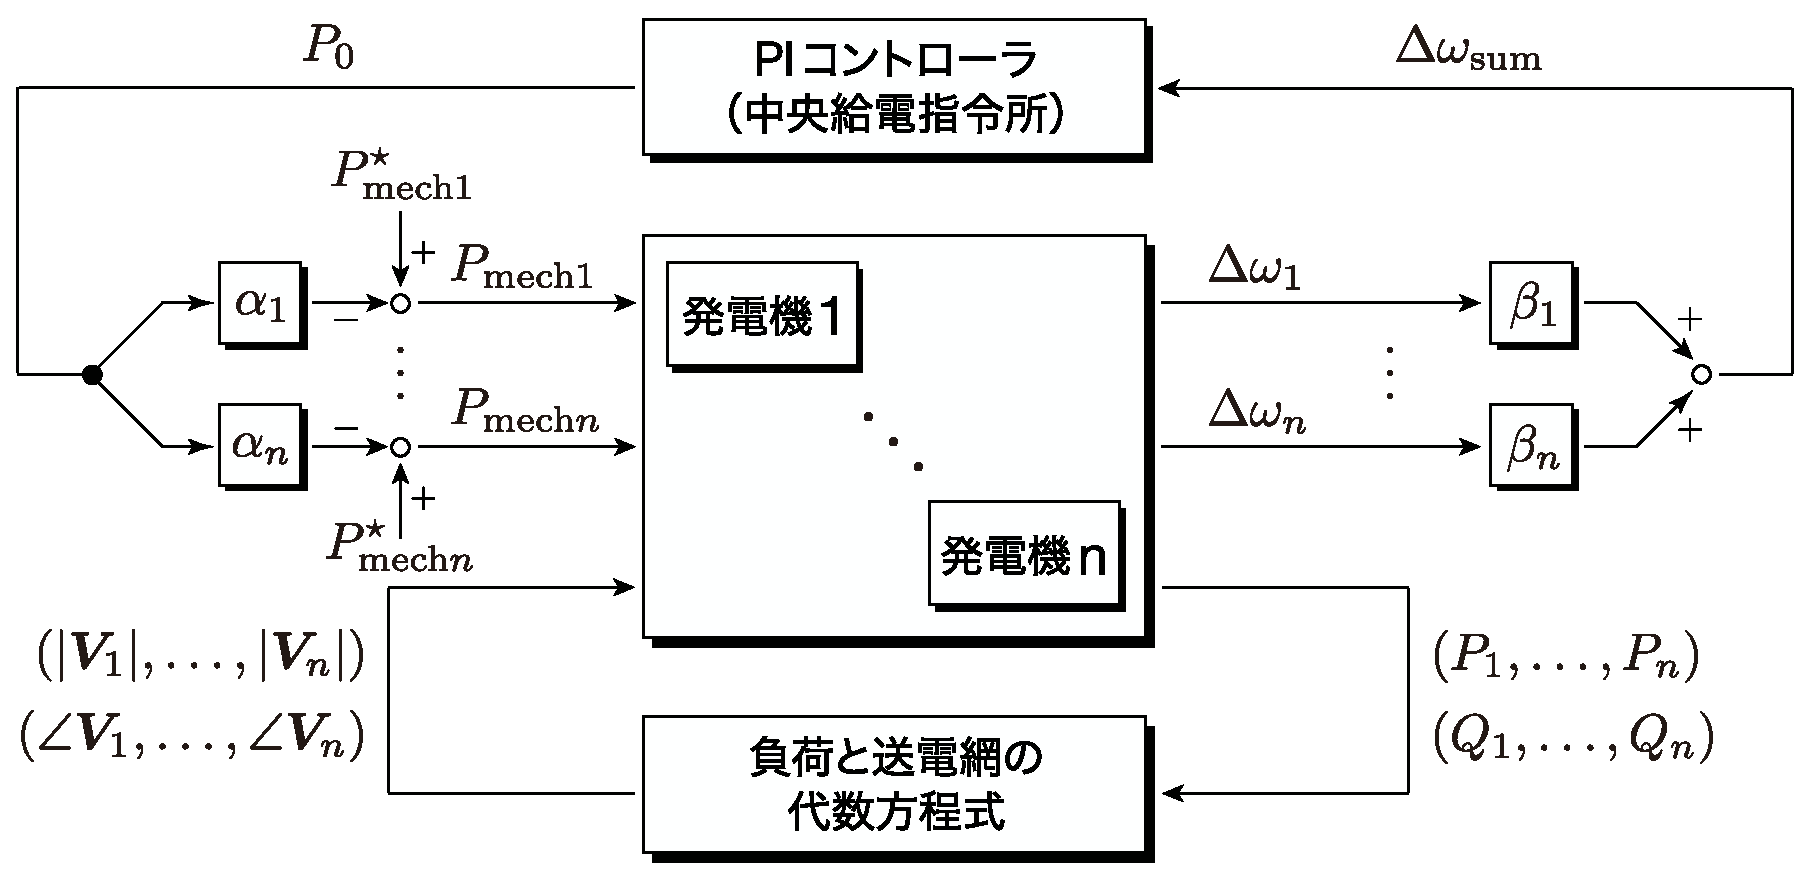
\includegraphics[width = .99\linewidth]{figs/bcAGC}
\medskip
\caption{\textbf{自動発電制御の信号伝達構造}}
\label{fig:bcAGC}
\medskip
\end{figure}

自動発電制御は,式(\ref{eq:gendifagc})の機械的トルク$P_{{\rm mech}i}$を調整する制御アルゴリズムである。
以下では,すべての発電機に関する周波数偏差の重み付き和を観測し,すべての発電機に対して適当に重み付けされた制御入力を送信するブロードキャスト型PIコントローラを考えよう。
具体的には,各$i\in \mathcal{I}_{\rm G}$について
\begin{subequations}\label{eq:agccon}
\begin{align}\label{eq:agccona}
P_{{\rm mech}i}(t)=
P_{{\rm mech}i}^{\star} - \alpha_i
\underbrace{
\left\{
k_{\rm P} \Delta \omega_{\rm sum}(t) +
k_{\rm I}
\int_0^t \Delta \omega_{\rm sum}(\tau) d \tau
\right\}
}_{P_{0}(t)}
\end{align}
とする。
ただし,$P_{{\rm mech}i}^{\star} $は機械的トルクの標準設定値を表す定数である。
また,$\alpha_i $は発電機$i$の寄与を指定する非負定数であり
\[
\Delta \omega_{\rm sum}(t) := 
\sum_{i =1}^n \beta_i \Delta \omega_{i}(t)
\]
は周波数偏差の非負定数$\beta_i$に関する重み付き和とする。
さらに,$k_{\rm P}$,$k_{\rm I}$はPIコントローラのゲインを表す正定数である。
この自動発電制御器は,$\alpha_i$や$\beta_i$の重み付けのもと,単一のPIコントローラによって生成された信号$P_0(t)$をすべての発電機に同時送信(ブロードキャスト)する構造をもつ(\FIGref{fig:bcAGC})。
なお,式\ref{eq:agccona}を微分方程式で表現すれば
\begin{align}
\simode{
\dot{\xi}&=  \Delta \omega_{\rm sum} \\
P_{{\rm mech}i} &= P_{{\rm mech}i}^{\star} - \alpha_i \left(k_{\rm P} \Delta \omega_{\rm sum} +  k_{\rm I} \xi \right)
}
\end{align}
\end{subequations}
である
\footnote{
現実の火力発電や原子力発電では,火力や原子力で発生させた高圧の蒸気によりタービンを回転させて
機械的トルクを発生させる\textbf{原動機}(prime mover)が存在する。
原動機には,発電機の回転速度を自動制御する\textbf{ガバナ}(governor)が組み込まれている。
より現実的な自動発電制御の解析には,中央給電指令所からの指令値を入力とし,発電機に与える機械的トルクを出力とする原動機モデルを考慮する必要がある\cite[3章]{taniguchi2011power}。
}。
電力系統工学では,非負定数$\alpha_i$は発電機$i$の\textbf{寄与係数}(participation factor)と呼ばれる。

寄与係数の比率を変えることにより,需給がバランスした定常潮流状態において,各々の発電機が供給する有効電力の値を調整することができる。
システム制御工学の観点では,コントローラの切り替えにより,電力系統モデルの安定な平衡点を移動させることとして解釈できる。
\ref{sec:staana}章で解析したように,電力系統の安定性は平衡点の選び方によって変化する。
また,電力系統全体の発電コストや送電損失の値も平衡点の選び方に依存する。
したがって,寄与係数を需要の分布に合わせて適切に切り替えることは,系統安定度の向上や経済的コストの低減などにつながる
\footnote{
現実の電力系統運用では,寄与係数の更新は数分から数十分程度の間隔で行われるのが一般的である\cite[第11.1節]{kundur1994power}。
電力系統工学の用語では,この寄与係数を更新するスキームは,\textbf{経済負荷配分制御}(EDC:Economic load Dispatching Control)と呼ばれる。
また,寄与係数を更新間隔の間で定数として用いる制御アルゴリズムは,\textbf{負荷周波数制御}(LFC:Load Frequency Control)と呼ばれる。
ただし,文献によって経済負荷配分制御と負荷周波数制御の明確な区別がない場合や,経済負荷配分制御を異なるスキームとする場合もあるため注意が必要である。
}
。


\subsection{周波数安定化制御の数値シミュレーション}

簡単な例を用いて周波数安定化制御の効果を確認してみよう。

\begin{例}[自動発電制御による周波数の安定化]\label{ex:agcdemo}
例\ref{ex:inires}で扱った3母線で構成される電力系統モデルを考えよう。
発電機や送電線の物理定数は例\ref{ex:inires}と同じ値に設定し,発電機の内部状態の初期値には,\ref{table:genst13b}の定常値を設定する。
また,界磁電圧は\ref{table:genst13b}の値で一定であるものととする。

母線2の負荷は定電力モデルに設定して,初期値として設定した定常潮流状態から,有効電力の消費量が1\%増加する場合を考える。
まず,自動発電制御が組み込まれておらず,発電機の機械的トルクが\ref{table:genst13b}の値で一定である場合の周波数偏差の時間応答を\FIGref{fig:agcPdemo}(a)に示す。
負荷による消費電力が増加することにより需給が均衡しないため,周波数偏差の定常値が0にならないことがわかる。

つぎに,式(\ref{eq:agccon})のブロードキャスト型PIコントローラを自動発電制御として組み込まれている場合の結果を\FIGref{fig:agcPdemo}(b)に示す。
ただし,コントローラのパラメータは\ref{table:agcpara}の(a)の値に設定している。
この図から,自動発電制御の効果により負荷の消費電力が変化しても周波数偏差がほとんど生じないことがわかる。
\end{例}


\begin{figure}[t]
  \centering
  {
  \begin{minipage}{0.49\linewidth}
    \centering
    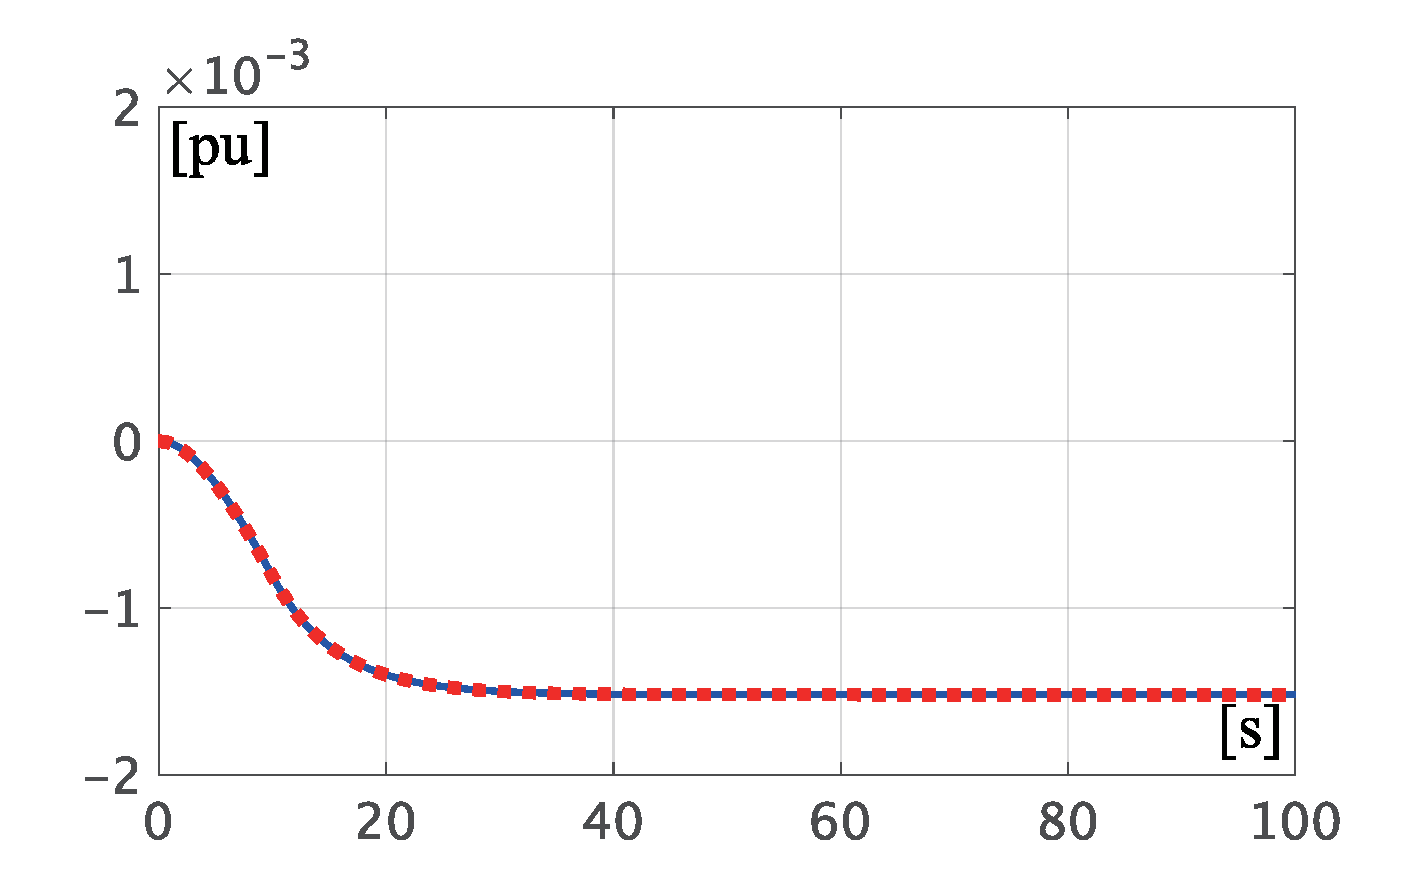
\includegraphics[width = 1.0\linewidth]{figs/woagcPinc}
    \subcaption{ 自動発電制御なし}
  \end{minipage}
  \begin{minipage}{0.49\linewidth}
    \centering
    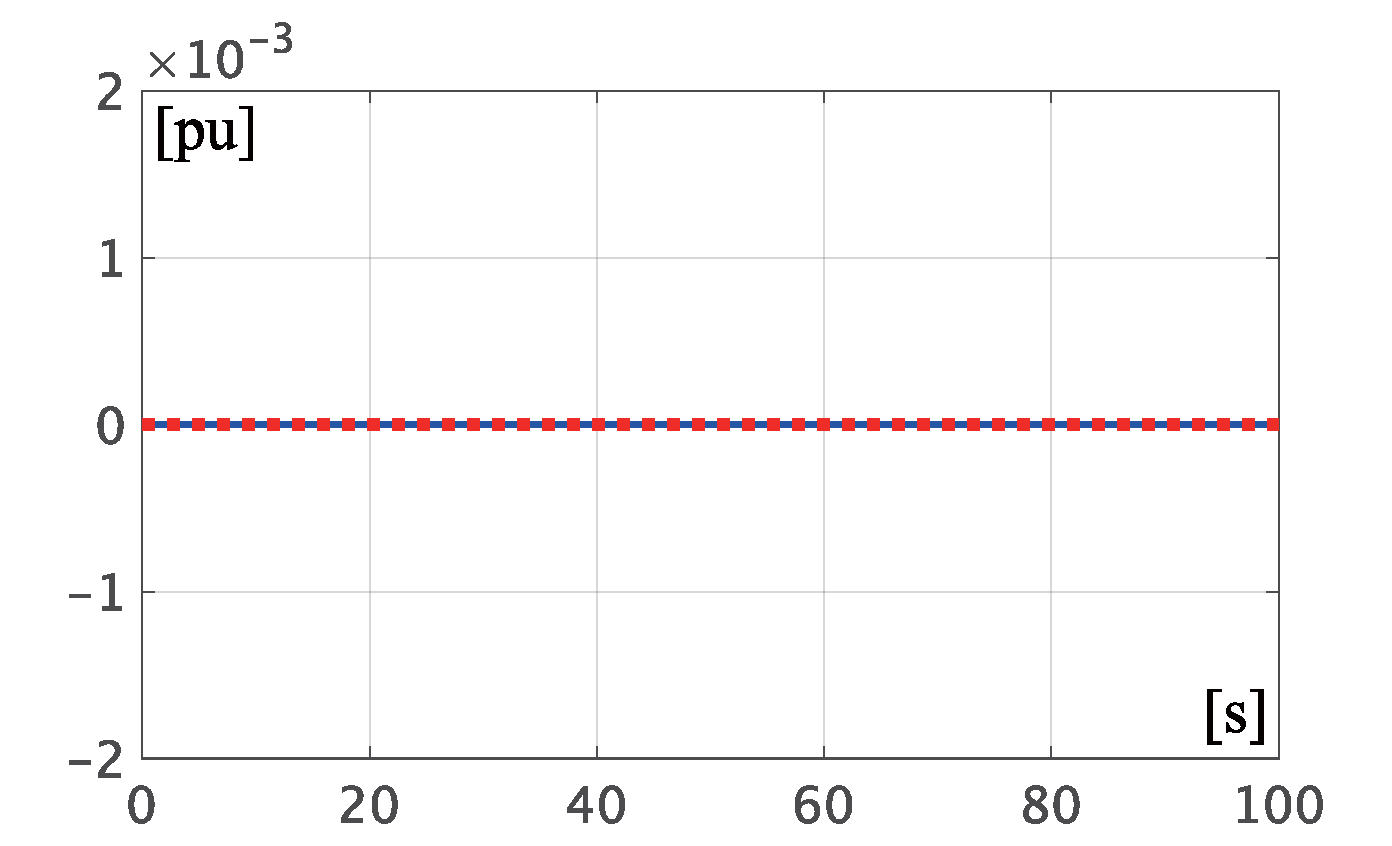
\includegraphics[width = 1.0\linewidth]{figs/wagcPinc}
    \subcaption{ 自動発電制御あり }
  \end{minipage}
  \medskip
  \caption{\textbf{消費電力の増加に対する周波数偏差の時間応答} }
  \label{fig:agcPdemo}
  }
\medskip
\end{figure}

\begin{table}[h]
\medskip
 \caption{\textbf{コントローラのパラメータ設定}}
 \label{table:agcpara}
 \centering
  \begin{tabular}{ccccccccc}
   \hline
設定 &  $k_{\rm P}$ & $k_{\rm I}$ & $\alpha_1$ & $\alpha_3$ &$\beta_1$ & $\beta_3$ \\
   \hline \hline
(a) & 100 & 500 & 1 & 3 & 1 & 3 \\
(b) & 100 & 500 & 1 & 1& 1 & 1 \\
(c) & 100 & 500 & 3 & 1 & 3 & 1 \\
   \hline
  \end{tabular}
\end{table}

つぎに,式(\ref{eq:agccon})におけるブロードキャスト型PIコントローラの寄与係数を調整することによって,需給バランスを達成する定常潮流状態が変化することを確認してみよう。

\begin{例}[寄与係数の調整による定常潮流状態の変化]\label{ex:pfvary}
例\ref{ex:agcdemo}と同様に,2つの発電機と1つ負荷で構成される電力系統モデルを考えよう。
ここでは,式(\ref{eq:agccon})におけるブロードキャスト型PIコントローラの寄与係数を変化させることで,発電機1と発電機3が供給する有効電力の比率が変化することを確認する。
具体的には,以下のように寄与係数を切り替える。
\begin{itemize}
\item 0~[s]から20~[s]の区間では\ref{table:agcpara}の(b)のパラメータを設定する。
\item 20~[s]から40~[s]の区間では\ref{table:agcpara}の(a)のパラメータを設定する。
\item 40~[s]から60~[s]の区間では\ref{table:agcpara}の(c)のパラメータを設定する。
\end{itemize}

得られた時間応答を\FIGref{fig:agcPvary}(a)に示す。
青の実線は発電機1が供給する有効電力$P_1$の値を表し,赤の破線は発電機3が供給する有効電力$P_3$の値を表す。
この結果から,定常潮流状態で実現される$P_1$と$P_3$の比率が,寄与係数の$\alpha_1$と$\alpha_3$の比率に一致していることがわかる。

つぎに,有効電力の送電損失を表す$P_1+P_2+P_3$の時間応答を\FIGref{fig:agcPvary}(b)に示す。
なお,$P_2$は負荷で消費される有効電力であり,その値は$-3$で一定である。
この図から,実現される定常潮流状態によって,有効電力の送電損失の大きさが異なっていることがわかる。
特に,ブロードキャスト型PIコントローラのパラメータを\ref{table:agcpara}の(a)の値に設定する場合,すなわち,母線2と母線3を端点とする抵抗のない送電線を主に用いて電力を供給する場合に,電力系統全体の送電損失がより小さくなることがわかる。
この結果は,例\ref{ex:pf3bus}で議論したことと同様である。
なお,送電線のアドミタンスは,式\ref{eq:rightlossless}の値に設定されている。
\end{例}

\begin{figure}[t]
  \centering
  {
  \begin{minipage}{0.49\linewidth}
    \centering
    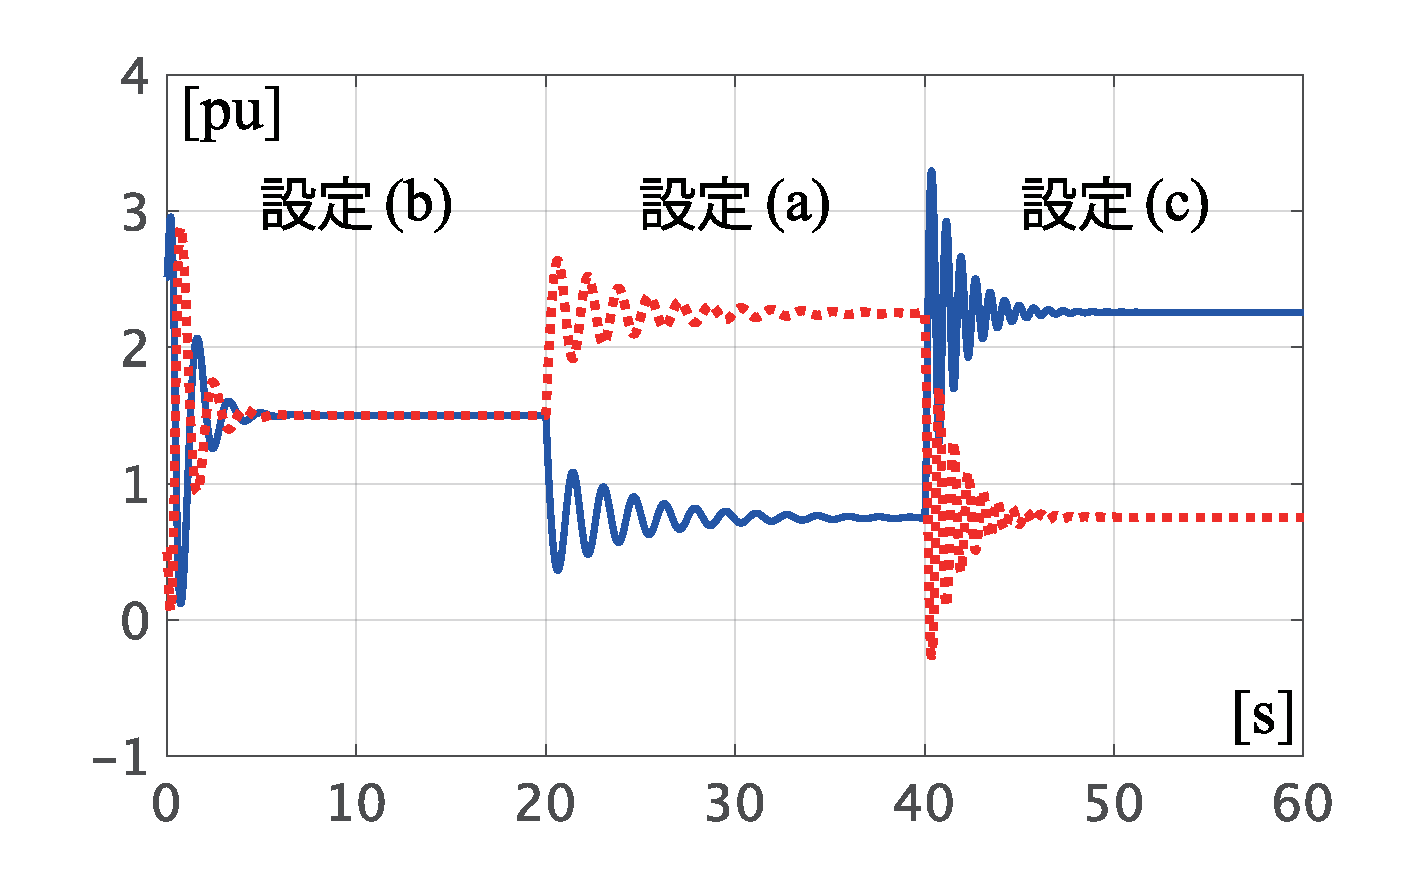
\includegraphics[width = 1.0\linewidth]{figs/varyalphaP}
    \subcaption{ 青実線:$P_1$,赤破線:$P_3$~[pu]}
  \end{minipage}
  \begin{minipage}{0.49\linewidth}
    \centering
    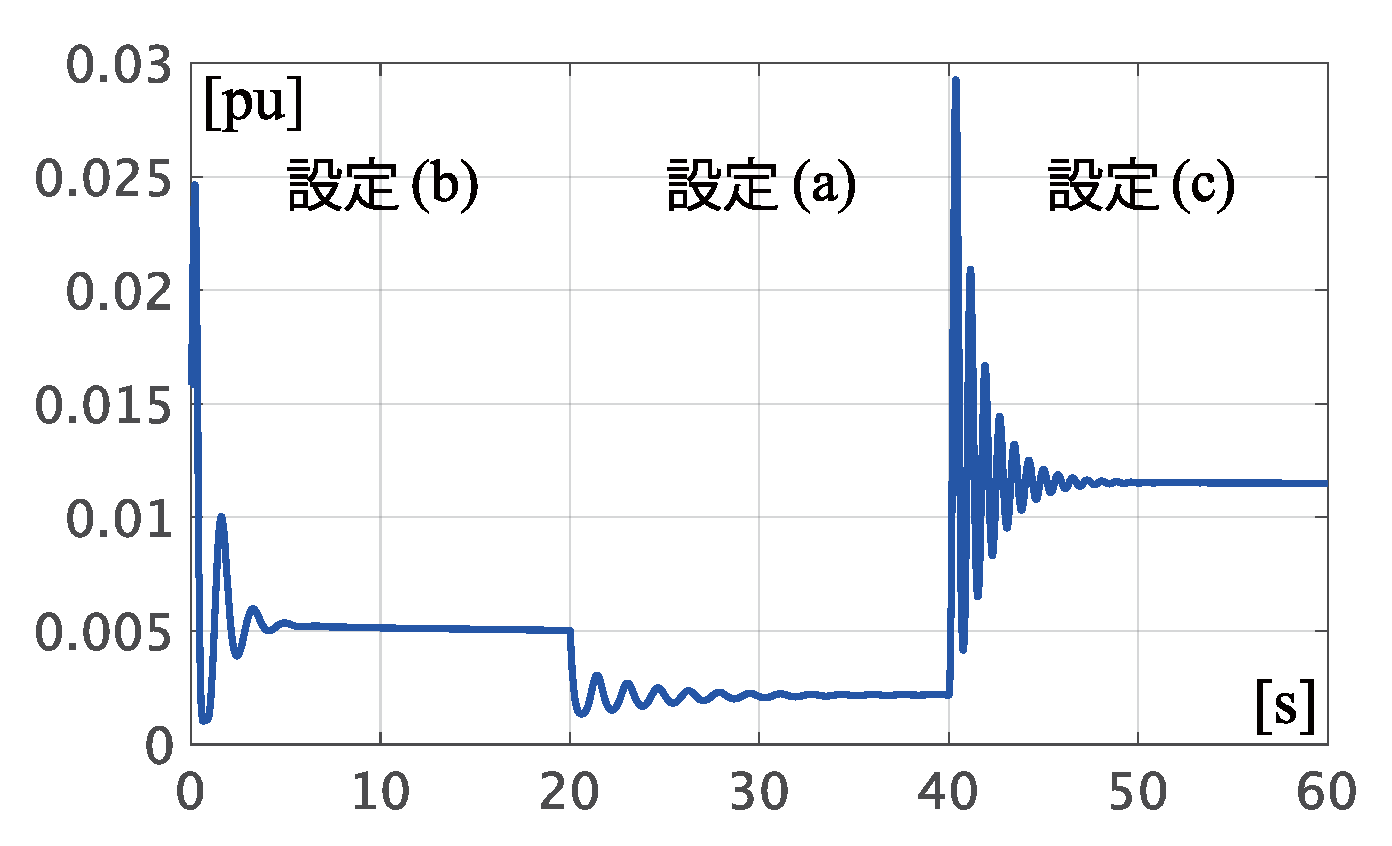
\includegraphics[width = 1.0\linewidth]{figs/varyalphaloss}
    \subcaption{ 送電損失$P_1+P_2+P_3$~[pu] }
  \end{minipage}
  \medskip
  \caption{\textbf{寄与係数の変化に対する有効電力の時間応答} }
  \label{fig:agcPvary}
  }
\medskip
\end{figure}


例\ref{ex:pfvary}で示されているように,ブロードキャスト型PIコントローラの寄与係数を調整することによって,実現する定常潮流状態を変化させることができる。
このとき,それぞれの定常潮流状態における送電損失の大きさや必要となる発電コストも変化する。
したがって,寄与係数を適切に制御することによって,より経済的な系統運用を実現することができる。
ただし,経済コストの低い定常潮流状態が必ずしも安定度の高い平衡点であるとは限らないため,経済性や安定度などに関するトレードオフを適切に考慮することが重要である。


\section{周波数安定化制御系の数学的な安定性解析\advanced}\label{sec:mathnpas}

\subsection{対象とする電力系統モデル\advanced}\label{sec:objmod}

\smallskip
\subsubsection{電力系統モデルと自動発電制御に関する仮定}

\ref{sec:stalin}節では,電力系統モデルが定常潮流状態の近傍にあることを仮定して近似線形モデルを導出し,定態安定性の必要条件や十分条件を解析した。
本節では,非線形系に対する同様の受動性の概念を用いて,微分代数方程式系として記述される電力系統モデルの周波数安定性を解析する。
特に,自動発電制御が組み込まれたフィードバック制御系全体の安定性を考える。
具体的には,以下の前提のもとで安定性解析を行う。
\begin{itemize}
\item すべての発電機は,式(\ref{eq:lmodelsagc})の発電機モデルで表される。
ただし,各発電機の界磁電圧は定数に設定されていることを仮定する。
\item すべての負荷は,式\ref{eq:contpwmod}の定電力モデルで表される。
\item 式\ref{eq:PQVgenagc}の送電網の代数方程式において,すべての送電線のコンダクタンスは0であることを仮定する。
\item 式(\ref{eq:agccon})のブロードキャスト型PIコントローラによって,自動発電制御が行われている。
ただし,寄与係数と周波数偏差の重みについて,すべての$i\in \mathcal{I}_{\rm G}$に対して,
$\alpha_i = \beta_i $
が成り立つことを仮定する。
\end{itemize}

1つ目と2つ目は,発電機と負荷の標準的なモデルを考えることを意味している。
3つ目の送電網に関する仮定は,送電損失が0であることを意味しており,数学的に安定性の解析を行うためには欠かすことができない
\footnote{
現実の電力系統では,送電損失を完全に0にすることはできないが,高電圧により少ない電流で電力を送ることで送電損失を低減することが可能である。
本節の議論は,近似的に送電損失が0とみなせるような高電圧による送電を前提にして,周波数安定性を解析することに相当する。
}
。
実際,送電損失がある場合には,電力系統モデルの安定性解析は数値的手法に頼らざるを得ないことが多くの文献で指摘されている\cite{narasimhamurthi1984existence,chang1995direct,chiang2011direct,yang2019distributed}。
また,4つ目の仮定は,ブロードキャスト型PIコントローラの入出力特性が受動的となるために必要である。
なお,少なくとも1つの$i\in \mathcal{I}_{\rm G}$に対して寄与係数$\alpha_i$が正であれば,いくつかの係数が0であっても構わない。


また,\ref{sec:phsync}節の解析で示されているように
\begin{itemize}
\item 定常潮流状態において,すべての発電機の周波数偏差は同じ値となる。
\end{itemize}
以下の周波数安定性の解析は,この事実を前提としている。
具体的には,ブロードキャスト型PIコントローラに含まれる1つの積分器のみによって,すべての発電機の定常的な周波数偏差を0とするためには,上記のような周波数偏差が自動的に同期する特性が必要となる。


\smallskip
\subsubsection{自動発電制御を組み込んだ電力系統のフィードバック系による表現}

\ref{sec:linpasana}節の議論と同様に,電力系統モデルを2つのサブシステムのフィードバック系として記述することを考える。
1つ目のサブシステムは
\begin{align}\label{eq:sys1}
\mathds{F}:
\simode{
M \Delta \dot{\omega}&= 
- 
D
\Delta\omega 
 + 
u_{\mathds{F}}
+P_{{\rm mech}}^{\star}
\\
y_{\mathds{F}}&= \omega_0 \Delta\omega 
}
\end{align}
とする。
ただし,$\Delta\omega$は$\Delta\omega_i$を縦に並べたベクトルであり,$M$と$D$は$M_i$と$D_i$を対角に並べた行列である。
また,$P_{{\rm mech}}^{\star}$は$P_{{\rm mech}i}^{\star}$を並べた定数ベクトルである。
この$\mathds{F}$は,定数ベクトル$P_{{\rm mech}}^{\star}$の違いを除いて,\ref{sec:linpasana}節の機械サブシステムに等しい。
2つ目のサブシステムは,\ref{sec:linpasana}節の電気サブシステムを非線形の微分代数方程式系で表現した
\begin{subequations}\label{eq:sys2G}
\begin{align}\label{eq:sys2}
\mathds{G}_i : 
\simode{ 
\dot{\delta}_i &= u_{\mathds{G}_i}
\\
\taudi \dot{E}_i & = 
 -\tfrac{ \Xsi }{ \Xti }E_i
+\left(
\tfrac{ \Xsi }{ \Xti }-1
\right)
|\bm{V}_i| \sfcos (\delta_i - \angle \bm{V}_i ) 
+ V_{{\rm field}i}^{\star}
\\
y_{\mathds{G}_i}&= \tfrac{E_i |\bm{V}_i|}{ \Xti} \sfsin (\delta_i - \angle \bm{V}_i)
}
\end{align}
である。
これは,発電機母線に関するサブシステムのように見えるが,式\ref{eq:sys2}における母線の電圧フェーザは,すべての発電機母線に関する連立方程式
\begin{align}\label{eq:gVeq}
\simode{
P_i &=
\sum_{i=1}^{N} B_{ij} |\bm{V}_i| |\bm{V}_j| \sfsin(\angle \bm{V}_i -\angle \bm{V}_j)
\\
Q_i &= 
 -\sum_{i=1}^{N} B_{ij} |\bm{V}_i| |\bm{V}_j| \sfcos(\angle \bm{V}_i -\angle \bm{V}_j)
}\qquad
i \in \mathcal{I}_{\rm G}
\end{align}
とすべての負荷母線に関する連立方程式
\begin{align}\label{eq:lVeq}
\simode{
&P_{{\rm load}i}^{\star} =
\sum_{i=1}^{N} B_{ij} |\bm{V}_i| |\bm{V}_j| \sfsin(\angle \bm{V}_i -\angle \bm{V}_j)
\\
&Q_{{\rm load}i}^{\star} = 
-\sum_{i=1}^{N} B_{ij} |\bm{V}_i| |\bm{V}_j| \sfcos(\angle \bm{V}_i -\angle \bm{V}_j)
}\qquad
i \in \mathcal{I}_{\rm L}
\end{align}
\end{subequations}
を同時に満たさなければならない。
ただし,式\ref{eq:gVeq}の有効電力$P_i$と無効電力$Q_i$は,式\ref{eq:PQoutagc}で定義される。
また,$B_{ij}$は,アドミタンス行列$\bm{Y}$の虚部であるサセプタンス行列の第$(i,j)$要素を表す。
以下では,すべての発電機母線$i \in \mathcal{I}_{\rm G}$に対して,式\ref{eq:sys2}から式\ref{eq:lVeq}をまとめたものを1つのサブシステムとみなし,それを電気サブシステム$\mathds{G}$と表す。

さらに,式(\ref{eq:agccon})のブロードキャスト型PIコントローラの動特性を
\begin{align}\label{eq:condsK}
\mathds{K}: \simode{
\dot{\xi}&=  h^{\sf T} u_{\mathds{K}} \\
y_{\mathds{K}} &= h \left(k_{\rm P} h^{\sf T}u_{\mathds{K}} +  k_{\rm I} \xi \right)
}
\end{align}
と表す。
ただし,$h$は$\alpha_i$を並べた列ベクトルである。
このとき,上記のサブシステム$\mathds{F}$,$\mathds{G}$とコントローラ$\mathds{K}$の入出力を
\begin{subequations}\label{eq:connds}
\begin{align}
u_{\mathds{F}} = - y_{\mathds{K}} + v_{\mathds{F}}&
,\qquad u_{\mathds{K}} = \frac{1}{\omega_0} y_{\mathds{F}}	\label{eq:connds1}
\\
u_{\mathds{G}} = y_{\mathds{F}}&
,\qquad
v_{\mathds{F}} = - y_{\mathds{G}}		\label{eq:connds2}
\end{align}
\end{subequations}
のように結合すれば,自動発電制御を組み込んだフィードバック制御系全体が表現できる。
ただし,$u_{\mathds{G}}$と$y_{\mathds{G}}$は$u_{\mathds{G}_i}$と$y_{\mathds{G}_i}$を並べたベクトルである。
フィードバック制御系全体のブロック線図を\FIGref{fig:nonlinBD}に示す。
なお,「電力バランスの方程式」のブロックに,負荷の消費電力や送電線のアドミタンスなどの未知なモデルパラメータが含まれることに注意されたい。

\begin{figure}[t]
\centering
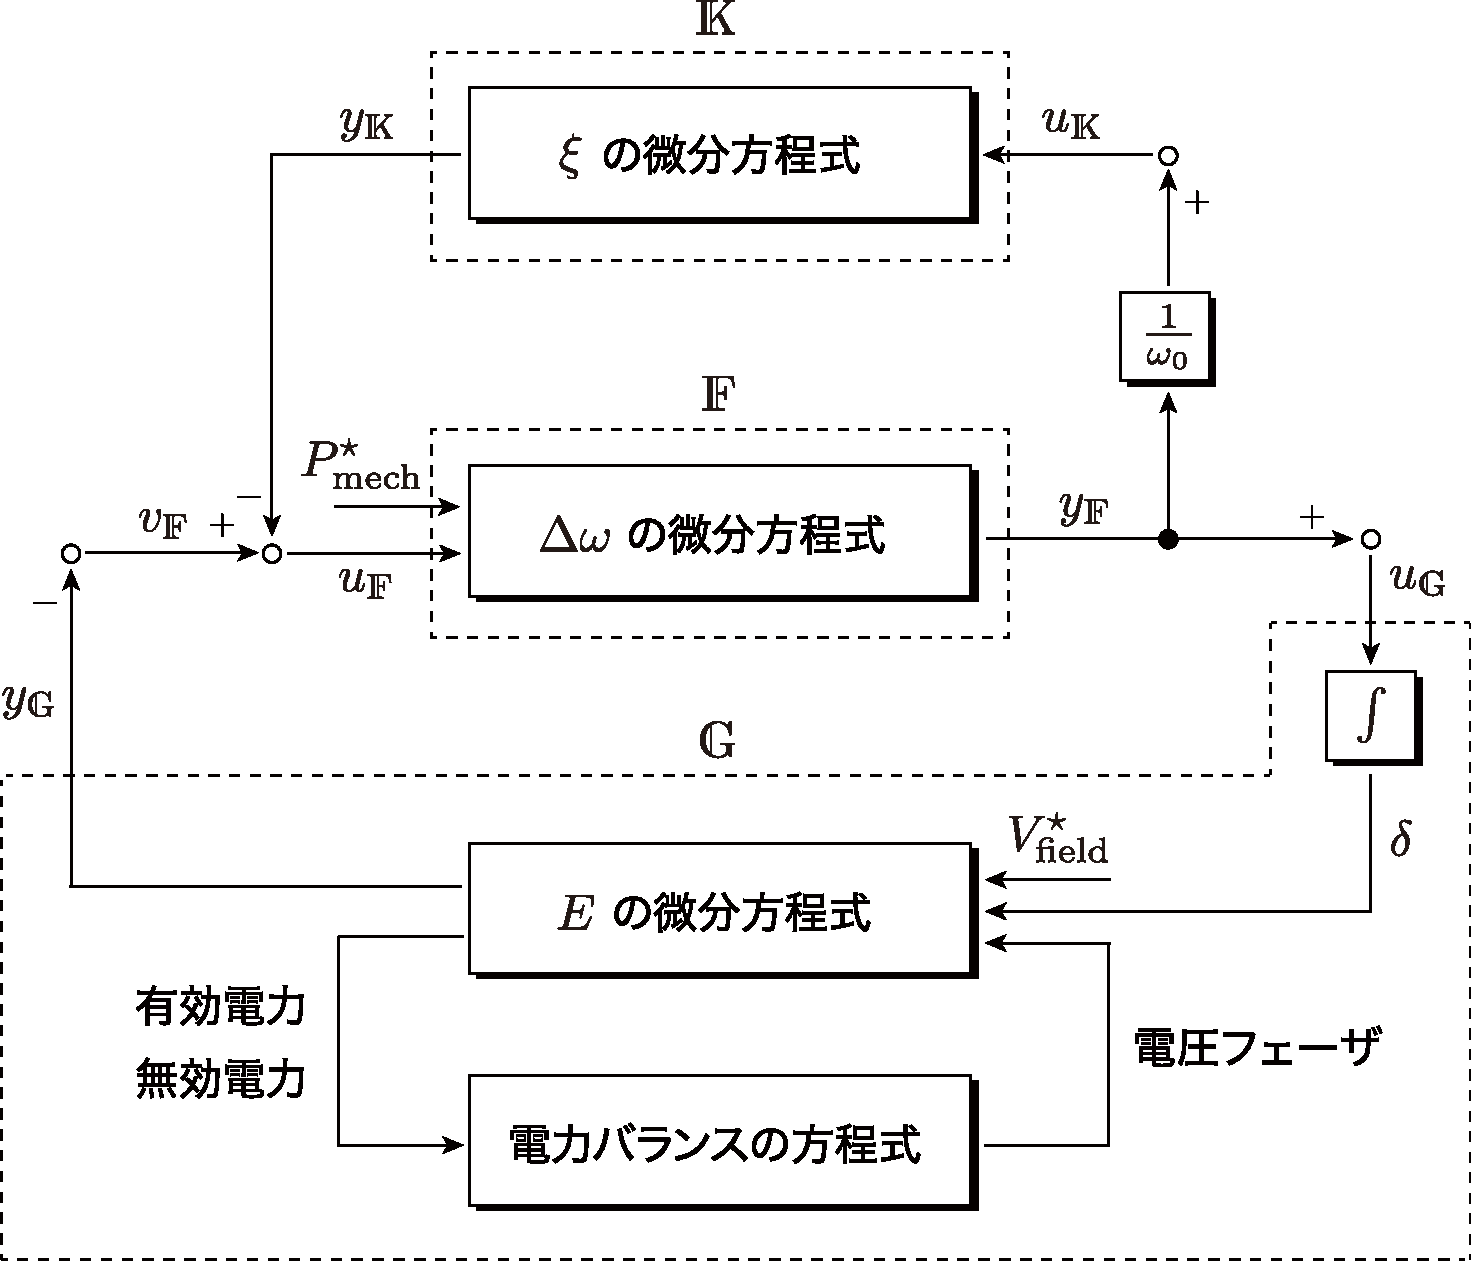
\includegraphics[width = .85\linewidth]{figs/nonlinBD}
\medskip
\caption{\textbf{自動発電制御を組み込んだフィードバック制御系}}
\label{fig:nonlinBD}
\medskip
\end{figure}



\subsection{電力系統モデルの平衡点に依らない受動性\advanced}

\smallskip
\subsubsection{平衡点に依らない受動性}

\ref{sec:linpasana}節の議論は,近似線形モデルによる解析であったため,その内部状態が0に漸近収束することが,もとの非線形モデルにおける特定の定常潮流状態への漸近収束を表していた。
一方で,非線形の微分代数方程式系として表現される電力系統モデルでは,電力の需要と供給がバランスする定常潮流状態においても内部状態は0とはならない。
さらに,定常潮流状態そのものが機械的トルクなどの設定値に依存して変化する。
したがって,個々の定常潮流状態(平衡点)の選択に依存しない安定性解析が望ましい。
このような解析を行うためにシステム制御工学で提唱されている概念として,\textbf{平衡点に依存しない受動性}(equilibrium-independent passivity)と呼ばれるものがある\cite{hines2011equilibrium,simpson2019equilibrium}。
なお,文献によっては,\textbf{シフトされた受動性}(shifted passivity)とも呼ばれている\cite{monshizadeh2019conditions}。
その定義はつぎのように与えられる。

\begin{定義}[平衡点に依らない受動性]\label{def:eipassive}
非線形システム
\begin{align}\label{eq:nlsig}
\Sigma: \simode{
E\dot{x} &= f(x) + Bu + R d^{\star}\\
y &= h(x)
}
\end{align}
を考える。
ただし,$f:\mathcal{X} \rightarrow \mathbb{R}^{n}$と$h:\mathcal{X} \rightarrow \mathbb{R}^{m}$は滑らかな関数であり,$B \in \mathbb{R}^{n\times m}$,$E \in \mathbb{R}^{n\times n}$,$R \in \mathbb{R}^{n\times p}$は行列である
\footnote{
行列$E$は,微分代数方程式系である式(\ref{eq:sys2G})の電気サブシステム$\mathds{G}$を表現するために導入した。
具体的には
\[
E=\mat{
I & 0 \\
0 & 0\\ 
}
\]
とすれば,式\ref{eq:nlsig}の$\Sigma$は,微分代数方程式系
\begin{align*}
\simode{
\dot{x}_1 &= f_1(x_1,x_2) + B_1u + R_1 d^{\star}\\
0 &= f_2(x_1,x_2) \\
y &= h(x_1,x_2)
}
\end{align*}
を表す。
電気サブシステム$\mathds{G}$に当てはめれば,$x_1$はすべての$\delta_i$と$E_i$を並べたベクトルであり,$x_2$はすべての$|\bm{V}_i|$と$\angle \bm{V}_i$を並べたベクトルである。
一方で,$E$が正則であるとき,式\ref{eq:sys1}の機械サブシステム$\mathds{F}$のような常微分方程式系を表す。
このようなシステム表現は,\textbf{ディスクリプタ形式}(descriptor representation)と呼ばれる。
}
。
また,$d^{\star}\in \mathbb{R}^p$ は定数ベクトルである。
なお,$\mathcal{X}$は許容可能な状態の領域である。
定常的な入力によって実現可能な平衡点の集合を
\begin{align*}%\label{eq:asbleq}
\mathcal{E}_{\Sigma} :=
\left\{
x^{\star} \in \mathcal{X}: 
\mbox{$0 = f(x^{\star})+B u^{\star}+ R d^{\star}$を満たす$u^{\star}$が存在する}
\right\}
\end{align*}
と表す。
各々すべての平衡点$x^{\star} \in \mathcal{E}_{\Sigma}$に対して,$W_{x^{\star}} (x^{\star})=0$であり,かつ,任意の入力$u $に対して
\begin{align*}%\label{eq:eiconpv}
\frac{d}{dt} W_{x^{\star}} \bigl( x(t) \bigr) \leq \bigl(u(t)-u^{\star}\bigr)^{\sf T} \bigl(y(t)-y^{\star}\bigr)
,\qquad
\forall t \geq 0
\end{align*}
を満たす微分可能な半正定値関数$W_{x^{\star}}:\mathcal{X} \rightarrow \mathbb{R}_{\geq 0}$が存在するとき,$\Sigma$は\textbf{平衡点に依らず受動的}であると呼ぶ。
ただし,平衡点$x^{\star}$における定常的な入力と出力を
\begin{align*}%\label{eq:uystar}
u^{\star} := -(B^{\sf T}B)^{-1}B^{\sf T} \bigl\{f(x^{\star}) + R d^{\star} \bigr\}
,\qquad
y^{\star} := h(x^{\star}) 
\end{align*}
と表している。
特に,上記の半正定値関数$W_{x^{\star}}(x)$に加えて
\begin{align*}%\label{eq:eiconosp}
\frac{d}{dt} W_{x^{\star}} \bigl( x(t) \bigr) \leq \bigl(u(t)-u^{\star}\bigr)^{\sf T} \bigl(y(t)-y^{\star}\bigr)
-\rho \bigl\|y(t)-y^{\star} \bigr\|^2
,\qquad
\forall t \geq 0
\end{align*}
を満たすある正定数$\rho$が存在するとき,$\Sigma$は\textbf{平衡点に依らず強受動的}であると呼ぶ。
\end{定義}

定義\ref{def:eipassive}では,システムの平衡点$x^{\star} \in \mathcal{E}_{\Sigma}$を基準としてその受動性が定義されていると解釈できる。
線形システムの範疇では,システムが零固有値をもたない限り,\ref{sec:linpasana}節の受動性の定義と等価であることが知られている\cite{hines2011equilibrium}。
なお,上記の関数$W_{x^{\star}}(x)$は,通常の受動性と同様に蓄積関数と呼ばれる。
この蓄積関数$W_{x^{\star}}(x)$は,平衡点$x^{\star}$の陰関数となっていることに注意されたい。

文献\cite{simpson2019equilibrium}において,システムが平衡点に依らず受動的である場合には,その蓄積関数はある関数$U(x)$を用いて
\begin{align}\label{eq:paraW}
W_{x^{\star}}(x) = U(x) - U(x^{\star}) - \nabla U^{\sf T}(x^{\star}) (x-x^{\star})
\end{align}
の形式で表せることが示されている
\footnote{
統計学などでは,凸関数である$U(x)$に対して,式\ref{eq:paraW}の右辺の量は$x$と$x^{\star}$の$U(x)$に関する\textbf{ブレグマン距離}(Bregman distance)と呼ばれている\cite{bregman1967relaxation}。
なお,$U(x)=\|x\|^2$とするとき,$W_{x^{\star}}(x)=\|x-x^{\star}\|^2$はユークリッド距離に一致する。
}
。
また,定義\ref{def:eipassive}では,式\ref{eq:paraW}の蓄積関数$W_{x^{\star}}(x)$は半正定値関数であることが条件として課されている。
具体的には
\begin{align}\label{eq:Uineqst}
U(x) \geq  U(x^{\star}) + \nabla U^{\sf T}(x^{\star}) (x-x^{\star})
\end{align}
が成り立つことが条件となる。
この不等式が任意の組$(x,x^{\star}) \in \mathcal{X} \times \mathcal{X}$に対して成り立つのであれば,各々すべての平衡点$x^{\star} \in \mathcal{E}_{\Sigma}$に対して,$W_{x^{\star}}(x)$は半正定値関数である。
式\ref{eq:Uineqst}の不等式は,$U(x)$が\textbf{凸関数}(convex function)であることを表す
\footnote{
関数$f(x)$に対して,定義域内から選ばれた任意の2点の組$(x,y)$について
\[
f\bigl(
\theta x + (1-\theta) y
\bigr)
\leq \theta f(x) + (1- \theta) f(y)
,\qquad
\forall \theta \in [0,1]
\]
が成り立つとき,$f(x)$は\textbf{凸関数}であると呼ぶ。
特に,$f(x)$が微分可能であるとき,$f(x)$が凸関数であるための必要十分条件は,任意の2点の組$(x,y)$について
\[
f(x) \geq f(y) + \nabla f^{\sf T}(y)(x-y)
\]
が成り立つことである。
}
。
後述するように,関数$U(x)$が凸であるような領域$\mathcal{X}$が,平衡点に依存しない受動性を用いた安定性解析に重要な役割を果たす。



\smallskip
\subsubsection{機械サブシステムの解析}

\ref{sec:linpasana}節で示されているように,機械サブシステム$\mathds{F}$は強受動的である。
同様に,式\ref{eq:sys1}の$\mathds{F}$が平衡点に依らず強受動的であることを確認する。
まず,機械サブシステムを
\begin{align}
\mathds{F}: \simode{
\dot{x}_{\mathds{F}} & = A_{\mathds{F}} x_{\mathds{F}} + B_{\mathds{F}} u_{\mathds{F}} 
+ R_{\mathds{F}} d_{\mathds{F}}^{\star} \\
y_{\mathds{F}} &= C_{\mathds{F}} x_{\mathds{F}}
}
\end{align}
の形式で書き表す。
ただし,状態$x_{\mathds{F}}$は$\Delta \omega_i$を並べたベクトルであり,
$u_{\mathds{F}}$と$y_{\mathds{F}}$は$u_{\mathds{F}_i}$と$y_{\mathds{F}_i}$を並べたベクトルである。
また,$d_{\mathds{F}}^{\star}$は$P_{\rm mech}^{\star}$を表し,システム行列は
\[
A_{\mathds{F}} := -M^{-1}D,\qquad
B_{\mathds{F}} := M^{-1},\qquad
R_{\mathds{F}} := M^{-1},\qquad
C_{\mathds{F}} := \omega_0 I
\]
である。
なお,行列$M$と$D$は,$M_i$と$D_i$を対角に並べた行列である。
任意に選ばれた平衡点$x^{\star}_{\mathds{F}} \in \mathcal{E}_{\mathds{F}}$に対して,蓄積関数を
\begin{align}\label{eq:WxFst}
W_{x^{\star}_{\mathds{F}}}(x_{\mathds{F}})
= \frac{\omega_0}{2}
(x_{\mathds{F}} -x^{\star}_{\mathds{F}})^{\sf T}
M
(x_{\mathds{F}} -x^{\star}_{\mathds{F}})
\end{align}
と選ぶ。
ただし,平衡点に関する$(x^{\star}_{\mathds{F}},u^{\star}_{\mathds{F}},y^{\star}_{\mathds{F}})$は
\begin{align}\label{eq:xFsteady}
0=
A_{\mathds{F}} x^{\star}_{\mathds{F}}
+
B_{\mathds{F}} u^{\star}_{\mathds{F}}
+ R_{\mathds{F}} d_{\mathds{F}}^{\star}
,\qquad
y^{\star}_{\mathds{F}} = C_{\mathds{F}} x^{\star}_{\mathds{F}}
\end{align}
を満たす。
なお,式\ref{eq:paraW}の形式で表すならば
\[
U_{\mathds{F}}(x_{\mathds{F}}):= \frac{\omega_0}{2} x_{\mathds{F}}^{\sf T} M x_{\mathds{F}}
\]
とすることにより,蓄積関数は
\[
W_{x^{\star}_{\mathds{F}}}(x_{\mathds{F}}) = U_{\mathds{F}}(x_{\mathds{F}}) 
- U_{\mathds{F}}(x^{\star}_{\mathds{F}}) 
- \nabla U^{\sf T}_{\mathds{F}}(x^{\star}_{\mathds{F}}) (x_{\mathds{F}}-x^{\star}_{\mathds{F}})
\]
と表せる。
この蓄積関数の勾配関数は
\begin{align*}%\label{eq:nabW}
\nabla W_{x^{\star}_{\mathds{F}}}(x_{\mathds{F}}) = \omega_0 M (x_{\mathds{F}} -x^{\star}_{\mathds{F}})
\end{align*}
であることから,蓄積関数の時間微分は
\begin{align}\label{eq:tdFds}
\spliteq{
\frac{d}{dt} W_{x^{\star}_{\mathds{F}}} \bigl( x_{\mathds{F}}(t) \bigr) 
&= 
\nabla W_{x^{\star}_{\mathds{F}}}^{\sf T}\left( x_{\mathds{F}}(t) \right) \dot{x}_{\mathds{F}}(t) \\
&= 
\nabla W_{x^{\star}_{\mathds{F}}}^{\sf T}\left( x_{\mathds{F}}(t) \right)
 \left\{
A_{\mathds{F}} \left( x_{\mathds{F}}(t) -x^{\star}_{\mathds{F}} \right)
+
B_{\mathds{F}} \left( u_{\mathds{F}}(t) -u^{\star}_{\mathds{F}} \right)
\right\}
\\
& \leq \textstyle
(y_{\mathds{F}}(t) -y^{\star}_{\mathds{F}})^{\sf T}
(u_{\mathds{F}}(t) -u^{\star}_{\mathds{F}})
 - \tfrac{\sfmin \left\{ D_i \right\}}{\omega_0}
\|y_{\mathds{F}}(t) -y^{\star}_{\mathds{F}}\|^2
}
\end{align}
と評価できる。
ただし,2つ目の等号の導出には,式\ref{eq:xFsteady}の関係を用いた。


\smallskip
\subsubsection{機械サブシステムと自動発電制御器のフィードバック系の解析}

機械サブシステムと同様にして,式\ref{eq:condsK}のブロードキャスト型PIコントローラの受動性も示すことができる。
蓄積関数を
\begin{align}\label{eq:Wxist}
W_{\xi^{\star}}(\xi) := \frac{1}{2} k_{\rm I} (\xi-\xi^{\star} )^2
\end{align}
と定義すれば,その時間微分は
\begin{align}\label{eq:tdKds}
\spliteq{
\frac{d}{dt} W_{\xi^{\star}} \bigl( \xi(t) \bigr) 
&=
(y_{\mathds{K}} - y_{\mathds{K}}^{\star})^{\sf T} (u_{\mathds{K}} - u_{\mathds{K}}^{\star})
- k_{\rm P} u_{\mathds{K}}^{\sf T} hh^{\sf T} u_{\mathds{K}} \\
& \leq (y_{\mathds{K}} - y_{\mathds{K}}^{\star})^{\sf T} (u_{\mathds{K}} - u_{\mathds{K}}^{\star})
}
\end{align}
と評価できる。
ただし,平衡点における$(\xi^{\star},u_{\mathds{K}}^{\star},y_{\mathds{K}}^{\star})$について
\begin{align}\label{eq:Kdseq}
\simode{
0 &=  h^{\sf T} u_{\mathds{K}}^{\star} \\
y_{\mathds{K}}^{\star} &= h \left(k_{\rm P} h^{\sf T}u_{\mathds{K}}^{\star} +  k_{\rm I} \xi^{\star} \right)
}
\end{align}
が成り立つことを用いた。

システム制御工学では,2つの受動的なシステムのネガティブ・フィードバック系は,再び受動的になることが知られている。
この事実に基づき,式\ref{eq:sys1}の機械サブシステム$\mathds{F}$と式\ref{eq:condsK}のブロードキャスト型PIコントローラ$\mathds{K}$をフィードバック結合した
\begin{align}\label{eq:sysFKds}
\mathds{F}_+:
\simode{
M \Delta \dot{\omega}&= 
- 
D
\Delta\omega 
- h \left(k_{\rm P} h^{\sf T}\Delta\omega  +  k_{\rm I} \xi \right)  + P_{{\rm mech}}^{\star} + v_{\mathds{F}}
\\
\dot{\xi} &= h^{\sf T}\Delta\omega\\
y_{\mathds{F}}&= \omega_0 \Delta\omega 
}
\end{align}
も平衡点に依らず強受動的であることが示される。
実際,式\ref{eq:tdFds}と式\ref{eq:tdKds}の不等式を足し合わせることにより
\begin{align}\label{eq:disineqFp}
\spliteq{
& \frac{d}{dt}  \left\{
W_{x^{\star}_{\mathds{F}}}  \bigl( x_{\mathds{F}}(t) \bigr) 
+
\omega_0
W_{\xi^{\star}} \bigl( \xi(t) \bigr) 
\right\} \\
& \hspace{3em} \leq 
(y_{\mathds{F}}(t) -y^{\star}_{\mathds{F}})^{\sf T}
(v_{\mathds{F}}(t) -v^{\star}_{\mathds{F}})  
- \tfrac{\sfmin \left\{ D_i \right\}}{\omega_0}
\|y_{\mathds{F}}(t) -y^{\star}_{\mathds{F}}\|^2
}
\end{align}
が得られる。
ただし,式\ref{eq:connds1}の入出力関係を用いた。

なお,式\ref{eq:connds2}の入出力関係により,式\ref{eq:sysFKds}の$\mathds{F}_+$と式(\ref{eq:sys2G})の$\mathds{G}$を結合すれば,自動発電制御を組み込んだフィードバック制御系全体が表される。
この事実に基づき,以下では$\mathds{G}$の平衡点に依らない受動性を解析する。

\smallskip
\subsubsection{電気サブシステムの解析}

式(\ref{eq:sys2G})の電気サブシステム$\mathds{G}$の平衡点に依らない受動性を解析する。
以下では,$\mathds{G}$の発電機母線と負荷母線に関する時間変数$\delta_i$,$E_i$,
$|\bm{V}_i|$,$\angle \bm{V}_i$をすべて並べた列ベクトルを$x_{\mathds{G}}$と表す。
この表記のもと,ポテンシャルエネルギー関数を
\begin{align}\label{eq:potWx}
\spliteq{
U_{\mathds{G}}(x_{\mathds{G}})  := 
&  \sum_{i=1}^n
\left\{
\frac{ \Xsi E_i^2 }{2 \Xti ( \Xsi - \Xti )}  
- 
\frac{E_i |\bm{V}_i|}{ \Xti } \sfcos (\delta_i - \angle \bm{V}_i)
+\frac{|\bm{V}_i|^2}{2 \Xti }
\right\}
\\
- & 
\sum_{i=1}^m
\left\{
 P_{{\rm load}i}^{\star} \angle \bm{V}_i
+ Q_{{\rm load}i}^{\star} \ln \left|\bm{V}_i \right|
\right\} \\
- & \sum_{i=1}^{N}
\sum_{j=1}^{N} \frac{B_{ij} }{2} |\bm{V}_i| |\bm{V}_j| \sfcos(\angle \bm{V}_i -\angle \bm{V}_j)
%\left\{
% \frac{B_{ii} }{2} |\bm{V}_i|^2  
%+ \sum_{j=1,j\neq i}^{N} \frac{B_{ij} }{2} |\bm{V}_i| |\bm{V}_j| \sfcos(\angle \bm{V}_i -\angle \bm{V}_j)
%\right\}
}
\end{align}
と定義する。
このポテンシャルエネルギー関数は,例えば\cite{tsolas1985structure,varaiya1985direct,chiang2011direct}において,1軸の発電機モデルと定電力の負荷モデルで構成される電力系統の安定性解析に用いられている。
ここで,式\ref{eq:paraW}の表現に基づいて,蓄積関数の候補を
\begin{align}\label{eq:stops}
W_{x^{\star}_{\mathds{G}}}(x_{\mathds{G}}) = U_{\mathds{G}}(x_{\mathds{G}}) 
- U_{\mathds{G}}(x^{\star}_{\mathds{G}}) 
- \nabla U_{\mathds{G}}^{\sf T}(x^{\star}_{\mathds{G}}) (x_{\mathds{G}}-x^{\star}_{\mathds{G}})
\end{align}
と構成する。
なお,その勾配関数は
\[
\nabla W_{x^{\star}_{\mathds{G}}}(x_{\mathds{G}}) =
\nabla U_{\mathds{G}}(x_{\mathds{G}}) 
- \nabla U_{\mathds{G}}(x^{\star}_{\mathds{G}}) 
\]
である。
蓄積関数の時間微分を計算するため,ポテンシャルエネルギー関数の勾配関数を求める。
まず,
$ U_{\mathds{G}}(x_{\mathds{G}}) $の$\delta_i$と$E_i$に関する偏微分を計算すると
\begin{align*}
\frac{\partial U_{\mathds{G}}}{\partial \delta_i}(x_{\mathds{G}}) &= \frac{E_i |\bm{V}_i|}{ \Xti } \sfsin (\delta_i - \angle \bm{V}_i) ,
\\
\frac{\partial U_{\mathds{G}}}{\partial E_i} (x_{\mathds{G}})&= - \frac{1}{ \Xsi - \Xti }
\left\{
-\frac{ \Xsi }{ \Xti }E_i
+\left(
\frac{ \Xsi }{ \Xti }-1
\right)
|\bm{V}_i| \sfcos (\delta_i - \angle \bm{V}_i ) 
\right\}
\end{align*}
となる。
したがって,各変数が式(\ref{eq:sys2G})の微分代数方程式にしたがうならば,式\ref{eq:sys2}から,すべての$i\in \mathcal{I}_{\rm G}$に対して
\begin{align*}
\frac{\partial U_{\mathds{G}}}{\partial \delta_i}(x_{\mathds{G}})  = y_{\mathds{G}_i}
,\qquad
\frac{\partial U_{\mathds{G}}}{\partial E_i} (x_{\mathds{G}})= 
\frac{V_{{\rm field}i}^{\star} - \taudi\dot{E}_i  }{ \Xsi - \Xti }
\end{align*}
が成り立つ。
また,$i\in \mathcal{I}_{\rm G}$に対して,電圧フェーザ変数に関するポテンシャルエネルギー関数の偏微分は
\begin{align*}
\spliteq{
\frac{\partial U_{\mathds{G}}}{\partial |\bm{V}_i| }(x_{\mathds{G}}) &= 
-
\sum_{j=1}^{N} B_{ij}  |\bm{V}_j| \sfcos(\angle \bm{V}_i -\angle \bm{V}_j)- \frac{Q_i}{|\bm{V}_i|}
\\
\frac{\partial U_{\mathds{G}}}{\partial \angle \bm{V}_i } (x_{\mathds{G}})&= 
\sum_{j=1}^{N}
B_{ij} |\bm{V}_i| |\bm{V}_j| \sfsin(\angle \bm{V}_i -\angle \bm{V}_j)
-
P_i
}
\end{align*}
となる。
したがって,式\ref{eq:gVeq}の方程式から,これらが0であることがわかる。
同様に,式\ref{eq:lVeq}の方程式から,$i\in \mathcal{I}_{\rm L}$に対して
\begin{align*}
\spliteq{
\frac{\partial U_{\mathds{G}}}{\partial |\bm{V}_i| }(x_{\mathds{G}}) &= 
- \sum_{j=1}^{N} B_{ij}  |\bm{V}_j| \sfcos(\angle \bm{V}_i -\angle \bm{V}_j)
 -  \frac{Q_{{\rm load}i}^{\star}}{|\bm{V}_i|}
\\
\frac{\partial U_{\mathds{G}}}{\partial \angle \bm{V}_i } (x_{\mathds{G}})&= 
\sum_{j=1}^{N} B_{ij} |\bm{V}_i| |\bm{V}_j| \sfsin(\angle \bm{V}_i -\angle \bm{V}_j)
-
P_{{\rm load}i}^{\star}
}
\end{align*}
も0であることがわかる。
したがって,すべての$i\in \mathcal{I}_{\rm G} \cup \mathcal{I}_{\rm L}$に対して
\begin{align*}
\frac{\partial U_{\mathds{G}}}{\partial |\bm{V}_i| } (x_{\mathds{G}})= 0
,\qquad
\frac{\partial U_{\mathds{G}}}{\partial \angle \bm{V}_i } (x_{\mathds{G}})= 0
\end{align*}
が成り立つことがわかる。

\begin{subequations}\label{eq:eqeq}
つぎに,$\nabla U_{\mathds{G}}(x^{\star}_{\mathds{G}}) $について,
$\mathds{G}$の定常状態に関する組$(x^{\star}_{\mathds{G}},u^{\star}_{\mathds{G}},y^{\star}_{\mathds{G}})$を考える。
平衡点の関係から,ある電圧フェーザ変数$(|\bm{V}_i^{\star}|, \angle \bm{V}_i^{\star})_{i\in \mathcal{I}_{\rm G} \cup \mathcal{I}_{\rm L} }$が存在して
\begin{align}\label{eq:eqeqa}
&\simode{
0 & = u_{\mathds{G}_i}^{\star} \\
 0 & =
-\tfrac{ \Xsi }{ \Xti }E_i^{\star}
+\left(
\tfrac{ \Xsi }{ \Xti }-1
\right)
|\bm{V}_i^{\star}| \sfcos (\delta_i^{\star} - \angle \bm{V}_i^{\star} ) 
+V_{{\rm field}i}^{\star}
} \\
&\simode{
P_i^{\star} 
& =
\sum_{j=1}^{N} B_{ij} |\bm{V}_i^{\star}| |\bm{V}_j^{\star}| \sfsin(\angle \bm{V}_i^{\star} -\angle \bm{V}_j^{\star})
\\
Q_i^{\star} 
&=
 - \sum_{j=1}^{N} B_{ij} |\bm{V}_i^{\star}| |\bm{V}_j^{\star}| \sfcos(\angle \bm{V}_i^{\star} -\angle \bm{V}_j^{\star})
}
\end{align}
が成り立つ。
ただし,$ i \in \mathcal{I}_{\rm G} $であり,有効電力と無効電力の定常値は
\begin{align*}%\label{eq:PQoutagcst}
\spliteq{
P_i^{\star}  &:=  \frac{E_i^{\star}  |\bm{V}_i^{\star} |}{ \Xti } 
\sfsin (\delta_i^{\star}  - \angle \bm{V}_i^{\star} ), \\
Q_i^{\star}  &:=  \frac{|\bm{V}_i^{\star} |E_i^{\star} }{ \Xti } 
\sfcos (\delta_i^{\star}  - \angle \bm{V}_i^{\star} )
-\frac{|\bm{V}_i^{\star} |^2}{ \Xti }
}
\end{align*}
である。
また,$y_{\mathds{G}_i}^{\star} = P_i^{\star}$である。
したがって,$ i \in \mathcal{I}_{\rm G} $に対して
\begin{align*}
\frac{\partial U_{\mathds{G}}}{\partial \delta_i}(x^{\star}_{\mathds{G}}) = y_{\mathds{G}_i}^{\star}
,\qquad
\frac{\partial U_{\mathds{G}}}{\partial E_i}(x^{\star}_{\mathds{G}}) = 
\frac{V_{{\rm field}i}^{\star}  }{ \Xsi - \Xti }
\end{align*}
が成り立つ。
同様に,すべての$ i \in \mathcal{I}_{\rm L} $に対して
\begin{align}
\simode{
&P_{{\rm load}i}^{\star}=
\sum_{j=1}^{N} B_{ij} |\bm{V}_i^{\star}| |\bm{V}_j^{\star}| \sfsin(\angle \bm{V}_i^{\star} -\angle \bm{V}_j^{\star}) 
\\
&Q_{{\rm load}i}^{\star}
=
-\sum_{j=1}^{N} B_{ij} |\bm{V}_i^{\star}| |\bm{V}_j^{\star}| \sfcos(\angle \bm{V}_i^{\star} -\angle \bm{V}_j^{\star})
}
\end{align}
\end{subequations}
が成り立つことから,母線の電圧フェーザ変数に関する偏微分は,すべての$i\in \mathcal{I}_{\rm G} \cup \mathcal{I}_{\rm L}$に対して
\begin{align*}
\frac{\partial U_{\mathds{G}}}{\partial |\bm{V}_i| }(x^{\star}_{\mathds{G}})= 0
,\qquad
\frac{\partial U_{\mathds{G}}}{\partial \angle \bm{V}_i } (x^{\star}_{\mathds{G}})= 0
\end{align*}
となる。
以上の計算結果より,蓄積関数の$\mathds{G}$の解軌道に沿った時間微分は
\begin{align}\label{eq:disineqGds}
\spliteq{
\frac{d}{dt}W_{x^{\star}_{\mathds{G}}} \bigl(x_{\mathds{G}}(t) \bigr)
& =
\nabla W_{x^{\star}_{\mathds{G}}}^{\sf T} \bigl(x_{\mathds{G}}(t) \bigr)
\dot{x}_{\mathds{G}}(t) \\
&=
\sum_{i=1}^n
\left(
(u_{\mathds{G}_i}- u_{\mathds{G}_i}^{\star}) (y_{\mathds{G}_i}-y_{\mathds{G}_i}^{\star})
-
\frac{\taudi}{ \Xsi - \Xti }
\dot{E}_i^2
\right)\\
& \leq 
(y_{\mathds{G}}-y_{\mathds{G}}^{\star})^{\sf T} (u_{\mathds{G}}- u_{\mathds{G}}^{\star})
}
\end{align}
と評価できる。
ただし,式\ref{eq:eqeqa}より,$u_{\mathds{G}}^{\star} = 0$であることを用いた。
このことから,式\ref{eq:stops}の関数$W_{x^{\star}_{\mathds{G}}}(x_{\mathds{G}})$が,電気サブシステム$\mathds{G}$の平衡点に依らない受動性に対する蓄積関数となることがわかる。
ただし,$x_{\mathds{G}}$や$x_{\mathds{G}}^{\star}$の領域は,$W_{x^{\star}_{\mathds{G}}}(x_{\mathds{G}})$が半正定値関数となる領域,すなわち,式\ref{eq:potWx}のポテンシャルエネルギー関数$U_{\mathds{G}}(x_{\mathds{G}})$が凸関数となる領域に限られることに注意されたい。
この点は次節で議論する。

\subsection{周波数安定化制御系の安定性解析\advanced}\label{sec:potconv}

\smallskip
\subsubsection{受動性に基づく未知平衡点の安定性解析}

以下では,平衡点に依らない受動性を用いて,\ref{sec:linmathana}節における近似線形モデルの受動性に基づく安定性解析と同様の手順により,自動発電制御が組み込まれたフィードバック制御系の安定性を解析する。
ただし,電気サブシステム$\mathds{G}$の解軌道$x_{\mathds{G}}(t)$に対して,式\ref{eq:stops}の蓄積関数の値$W_{x^{\star}_{\mathds{G}}}\bigl(x_{\mathds{G}}(t) \bigr)$が,すべての時刻$t$で非負となることを仮定して議論を進める。
この点は次項で議論する。

式\ref{eq:disineqFp}と式\ref{eq:disineqGds}の不等式の和に対して,式\ref{eq:connds2}の結合の関係を用いると,フィードバック制御系全体に対して
%\begin{align}\label{eq:disineqall}
%\spliteq{
%& \frac{d}{dt}  \left\{
%W_{x^{\star}_{\mathds{F}}}  \bigl( x_{\mathds{F}}(t) \bigr) 
%+
%\omega_0
%W_{\xi^{\star}} \bigl( \xi(t) \bigr) 
%+
%W_{x^{\star}_{\mathds{G}}} \bigl(x_{\mathds{G}}(t) \bigr)
%\right\} \\
%& \hspace{3em} \leq 
%(y_{\mathds{F}}(t) -y^{\star}_{\mathds{F}})^{\sf T}
%(v_{\mathds{F}}(t) -v^{\star}_{\mathds{F}})  
%- \tfrac{\sfmin \left\{ D_i \right\}}{\omega_0}
%\|y_{\mathds{F}}(t) -y^{\star}_{\mathds{F}}\|^2
%}
%\end{align}
\[
 \frac{d}{dt}  \left\{
W_{x^{\star}_{\mathds{F}}}  \bigl( x_{\mathds{F}}(t) \bigr) 
+
\omega_0
W_{\xi^{\star}} \bigl( \xi(t) \bigr) 
+
W_{x^{\star}_{\mathds{G}}} \bigl(x_{\mathds{G}}(t) \bigr)
\right\} 
 \leq 
- \tfrac{\sfmin \left\{ D_i \right\}}{\omega_0}
\|y_{\mathds{F}}(t) -y^{\star}_{\mathds{F}}\|^2
\]
が得られる。
この不等式から蓄積関数の和は単調非増加であることがわかる。
また,その下限値は 0 であることから,時間が十分に経過するとその和はある値に漸近収束する。
すなわち,左辺の時間微分は0に漸近収束する。
したがって
\[
\lim_{t\rightarrow \infty}
y_{\mathds{F}}(t) = y^{\star}_{\mathds{F}}
\]
が導かれる。
また,式\ref{eq:sys1}の出力方程式に注目すると,出力$y_{\mathds{F}}$は内部状態$\Delta \omega$の定数倍であることから,機械サブシステム$\mathds{F}$に対して
\begin{align}\label{eq:Fobsnl}
y_{\mathds{F}}(t)  =y^{\star}_{\mathds{F}},\quad \forall t\geq 0 
\qquad \Longrightarrow \qquad
\Delta \omega(t)  =\frac{1}{\omega_0} y^{\star}_{\mathds{F}},\quad \forall t\geq 0 
\end{align}
が成り立つ。
さらに,\ref{sec:phsync}節で解析したように,すべての発電機の周波数偏差は同じ値に収束する。
この事実は,ある定数$\gamma_0$に対して
\[
y^{\star}_{\mathds{F}} = \gamma_0 \mathds{1}
\]
であることを意味する。
一方で,式\ref{eq:Kdseq}の第1式から
\[
0=h^{\sf T} u_{\mathds{K}}^{\star} 
= \frac{1}{\omega_0}h^{\sf T} y^{\star}_{\mathds{F}}
=\frac{\gamma_0}{\omega_0} h^{\sf T} \mathds{1}
\]
となる。
ここで,$h^{\sf T} \mathds{1}\neq 0$であることから,$\gamma_0=0$が得られる。
以上より
\[
\lim_{t\rightarrow \infty}
\Delta \omega (t) = 0
\]
が示される。
また,すべての$i\in \mathcal{I}_{\rm G}$に対して
\[
\lim_{t\rightarrow \infty}
P_{{\rm mech}i}(t) 
=
\lim_{t\rightarrow \infty} P_i (t)
\]
が成り立つこともわかる。
ただし,これらの収束値は,負荷の消費電力や送電線のインピーダンスなどが現実的には未知であるため,事前に計算することは一般に不可能な値である。
同様に,式(\ref{eq:sys2G})の電気サブシステム$\mathds{G}$の内部状態や母線の電圧フェーザ変数も未知の値に漸近収束する。


\begin{table}[h]
\medskip
\caption{\textbf{初期値に設定する定常潮流状態}} \label{table:pflownl}
 \centering
  {
  \begin{minipage}{0.49\linewidth}
    \centering
  \begin{tabular}{|c|c|c|c|c|c|c|}
   \hline
 &  母線1 & 母線2 & 母線3 \\
   \hline 
   $P_i^{\star}$ & 2.5000 & $-3$ & 0.5 \\
   \hline
   $Q_i^{\star}$ & 0.1044 & 0 & 0.0365 \\
   \hline
   $|\bm{V}_i^{\star}|$ & 2 & 1.9984 & 2 \\
   \hline
   $\angle \bm{V}_i^{\star}$ & 0 & $-0.0539$ & $-0.0420$ \\
   \hline
  \end{tabular}
  \subcaption{定常潮流状態1}
  \end{minipage}
  \begin{minipage}{0.49\linewidth}
    \centering
  \begin{tabular}{|c|c|c|c|c|c|c|}
   \hline
 &  母線1 & 母線2 & 母線3 \\
   \hline 
   $P_i^{\star}$ & 0.5 & $-3$ & 2.5000 \\
   \hline
   $Q_i^{\star}$ & 0.0432 & 0 & 0.1111 \\
   \hline
   $|\bm{V}_i^{\star}|$ & 2 & 1.9983 & 2 \\
   \hline
   $\angle \bm{V}_i^{\star}$ & $-0.0488$ & $-0.0595$ & 0 \\
   \hline
  \end{tabular}
   \subcaption{定常潮流状態2}
  \end{minipage}
  }
\end{table}

\begin{例}[蓄積されるエネルギーの時間変化]\label{ex:nonlinene}
例\ref{ex:agcdemo}や例\ref{ex:pfvary}と同様に,2つの発電機と1つの定電力モデルの負荷で構成される電力系統モデルを考えよう。
ただし,送電線のアドミタンス値は,式\ref{eq:defadpara}や式\ref{eq:rightlossless}において,コンダクタンス成分を0とした式\ref{eq:bothlossless}の値に設定する。
また,発電機の物理定数や界磁電圧,初期値などは,例\ref{ex:agcdemo}や例\ref{ex:pfvary}と同様に設定する。
式(\ref{eq:agccon})のブロードキャスト型PIコントローラには,\ref{table:agcpara}の(b)のパラメータを設定する。

発電機の初期値には,\ref{table:pflownl}に示される2通りの定常潮流状態に対応する定常値を設定する。
それぞれの初期値に対する電力系統の時間応答について,式\ref{eq:WxFst}の$W_{x^{\star}_{\mathds{F}}}(x_{\mathds{F}})$,
式\ref{eq:Wxist}の$W_{\xi^{\star}}(\xi)$,式\ref{eq:stops}の$W_{x^{\star}_{\mathds{G}}}(x_{\mathds{G}})$の値を計算した結果が\FIGref{fig:LyapWnlin}の(a)と(b)である。
青,赤,緑の実線はそれぞれ,$W_{x^{\star}_{\mathds{F}}}(x_{\mathds{F}})$,$W_{x^{\star}_{\mathds{G}}}(x_{\mathds{G}})$,$W_{\xi^{\star}}(\xi)$を表す。
また,黒の破線はそれらの総和を表す。
これらの図から,3者の間でエネルギーを交換しながら,電力系統全体の総エネルギーが単調に減少していることがわかる。
\end{例}


\begin{figure}[t]
  \centering
  {
  \begin{minipage}{0.49\linewidth}
    \centering
    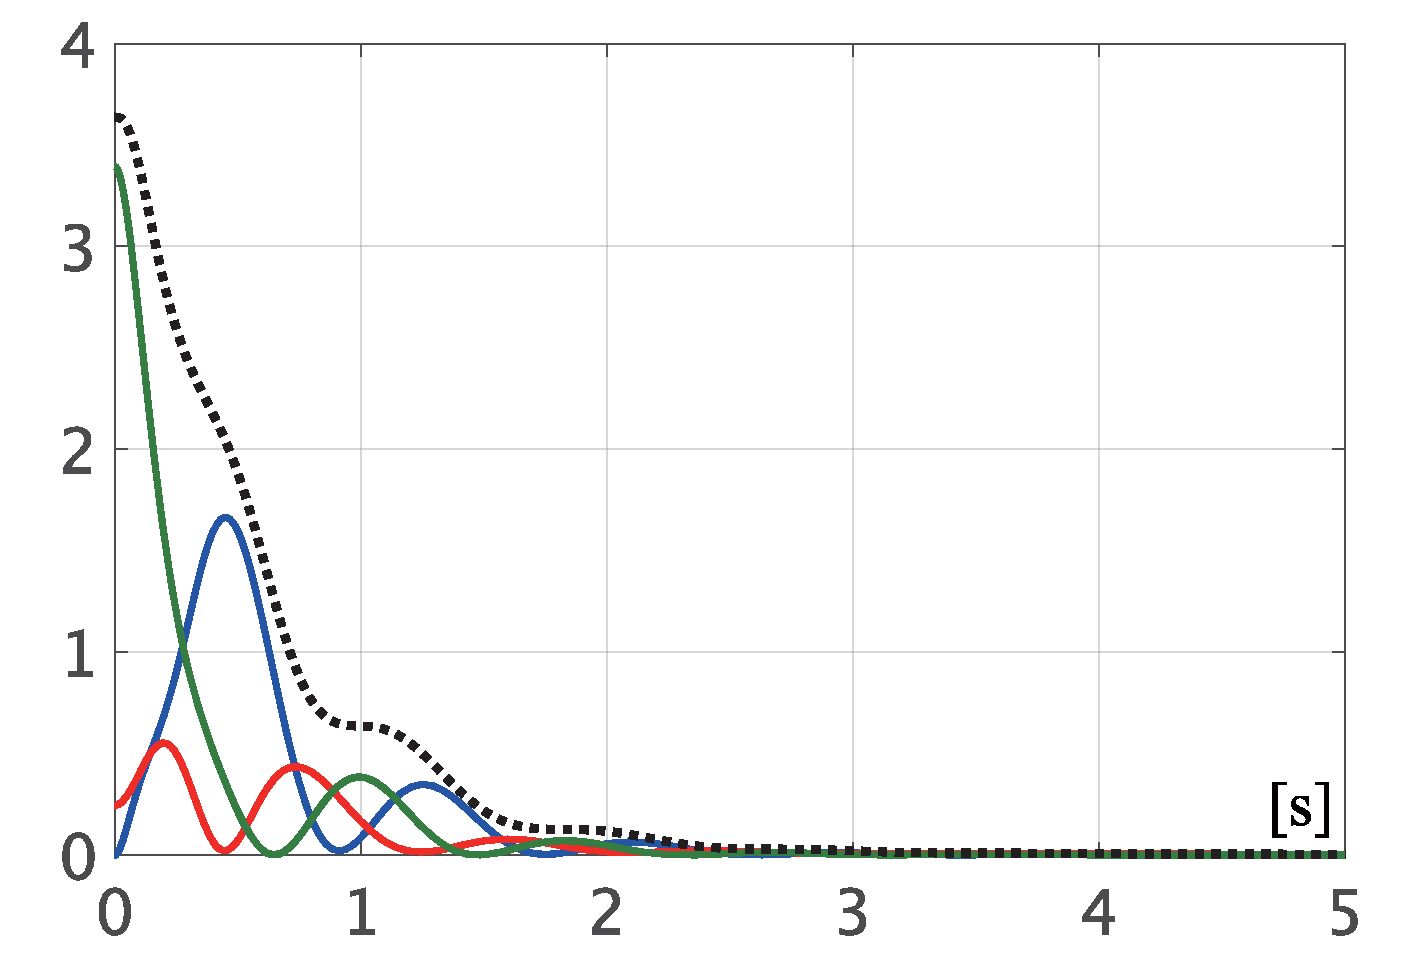
\includegraphics[width = 1.0\linewidth]{figs/Wnlin1}
    \subcaption{定常潮流状態1に対応する初期値 }
%    \medskip
  \end{minipage}
  \begin{minipage}{0.49\linewidth}
    \centering
    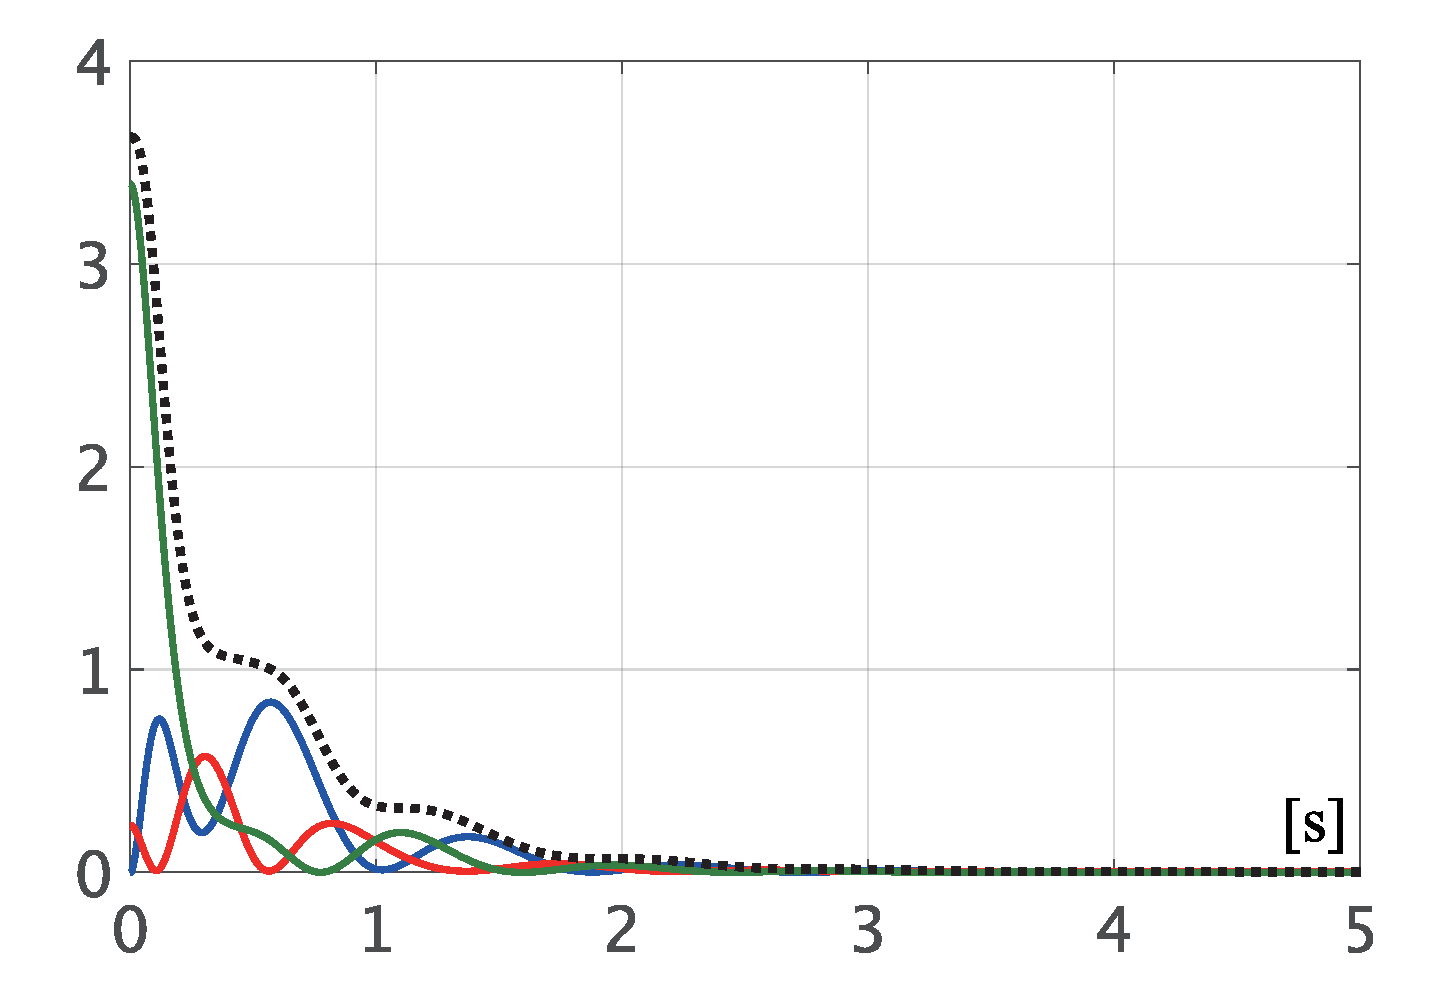
\includegraphics[width = 1.0\linewidth]{figs/Wnlin2}
    \subcaption{定常潮流状態2に対応する初期値 }
%    \medskip
  \end{minipage}
  }
  \medskip
  \caption{\textbf{初期値応答に対する蓄積関数の時間変化}
  \\  \centering(青:$W_{x^{\star}_{\mathds{F}}}$,赤:$W_{x^{\star}_{\mathds{G}}}$,
  緑:$W_{\xi^{\star}}$,黒:総和)}
  \label{fig:LyapWnlin}
\medskip
\end{figure}



%式(\ref{eq:sys2G})の電気サブシステム$\mathds{G}$の平衡点に依らない受動性を解析する。
%以下では,$\mathds{G}$のすべての時間変数である$(\delta_i, E_i)_{i\in \mathcal{I}_{\rm G}}$と
%$(|\bm{V}_i|, \angle \bm{V}_i)_{i\in \mathcal{I}_{\rm G} \cup \mathcal{I}_{\rm L}}$を並べた列ベクトルを$x_{\mathds{G}}$と表す。
%
%
%なお,ここまでの議論の結果から,式(\ref{eq:connds})における入出力信号はそれらの定常値
%\[
%u_{\mathds{F}}^{\star} =0
%,\qquad
%y_{\mathds{F}}^{\star} =0
%,\qquad
%u_{\mathds{K}}^{\star} =0
%,\qquad
%y_{\mathds{K}}^{\star} =v_{\mathds{F}}^{\star}
%= -y_{\mathds{G}}^{\star}
%,\qquad
%u_{\mathds{G}}^{\star} =0
%\]
%に漸近収束することもわかる。

\smallskip
\subsubsection{ポテンシャルエネルギー関数が凸となる領域}

以下では,式\ref{eq:potWx}のポテンシャルエネルギー関数$U_{\mathds{G}}(x_{\mathds{G}})$が凸関数となるための条件が,近似線形モデルの受動性解析で議論した定義\ref{def:passtrans}の受動送電条件(i)と(iii)に対応することを示そう。
なお,本節の議論では,受動送電条件(ii)は仮定されている。

\ref{sec:linpasana}節の近似線形モデルの設定に合わせて,すべての母線に発電機が接続されている場合を考える。
すなわち,発電機母線と負荷母線の添字集合は
\[
\mathcal{I}_{\rm G} = \{1,\ldots,N\}
,\qquad
\mathcal{I}_{\rm L} = \emptyset
\]
である。
このとき,発電機母線のクロン縮約を適用することにより,式(\ref{eq:sys2G})の電気サブシステム$\mathds{G}$と等価な常微分方程式系が,$i \in \mathcal{I}_{\rm G}$に関する
\begin{align*}%\label{eq:kronGds}
\mathds{G}_i : 
\simode{
\dot{\delta}_i &= u_{\mathds{G}_i}
\\
\taudi \dot{E}_i & = 
 -\tfrac{ \Xsi }{ \Xti }E_i
 - \left(
\Xsi - \Xti
\right)
\sum_{j=1}^{N}
E_j 
B_{ij}^{\rm red}
\sfcos \delta_{ij}
+ V_{{\rm field}i}^{\star}
\\
y_{\mathds{G}_i}&=  -E_i \sum_{j=1}^{N}
 E_j 
B_{ij}^{\rm red}
\sfsin \delta_{ij}
}
\end{align*}
と得られる。
ただし,$\delta_{ij}:= \delta_i -\delta_j$である。
また,縮約サセプタンス$B_{ij}^{\rm red}$は,式(\ref{eq:sys2G})の$B_{ij}$をまとめた送電網のサセプタンス行列を$B$と表すとき
\[
B^{\rm red}
:= -
\bigl\{
\sfdiag \left( \Xti \right)   
-
\sfdiag \left( \Xti \right) B \sfdiag \left( \Xti \right)
\bigr\}^{-1}
\]
の第$(i,j)$要素として定義される
\footnote{
この縮約サセプタンス行列$B^{\rm red}$のすべての要素は非正である。
この事実は,以下のように示される。
\ref{sec:admathp}節の議論から,サセプタンス行列$B$は非対角要素が非負の負定行列である。
したがって
\[
B_{-}:= \sfdiag \left( \Xti \right)   
-
\sfdiag \left( \Xti \right) B \sfdiag \left( \Xti \right)
\]
は非対角要素が非正の正定行列である。
このような行列は,\textbf{M行列}(M-matrix)と呼ばれる。
また,その逆行列の要素はすべて非負であることが知られている\cite{kodama1981system}。
したがって,$B^{\rm red}=-B_-^{-1}$のすべての要素は非正となる。
}
。
この常微分方程式系表現に対応する式\ref{eq:potWx}のポテンシャルエネルギー関数は
\begin{align}\label{eq:potWxred}
U_{\mathds{G}}^{\rm red} (z_{\mathds{G}})  := 
 \frac{1}{2} 
\sum_{i=1}^N
\left\{
\frac{ \Xsi E_i^2 }{ \Xti ( \Xsi - \Xti )}  
+ E_i \sum_{j=1}^{N}
 E_j 
B_{ij}^{\rm red}
\sfcos \delta_{ij}
\right\}
\end{align}
となる。
ただし,すべての$\delta_i$と$E_i$を並べたベクトルを$z_{\mathds{G}}$と表している。
内部状態に関する偏微分を計算すると
\begin{align*}
\frac{\partial U_{\mathds{G}}^{\rm red} }{\partial \delta_i}(z_{\mathds{G}})  = y_{\mathds{G}_i}
,\qquad
\frac{\partial U_{\mathds{G}}^{\rm red} }{\partial E_i} (z_{\mathds{G}}) = 
\frac{V_{{\rm field}i}^{\star} - \taudi\dot{E}_i  }{ \Xsi - \Xti }
\end{align*}
が得られる。
同様に,定常状態に対して
\begin{align*}
\frac{\partial U_{\mathds{G}}^{\rm red} }{\partial \delta_i} ( z^{\star}_{\mathds{G}} )
= y_{\mathds{G}_i}^{\star}
,\qquad
\frac{\partial U_{\mathds{G}}^{\rm red} }{\partial E_i} ( z^{\star}_{\mathds{G}} ) = 
\frac{V_{{\rm field}i}^{\star}  }{ \Xsi - \Xti }
\end{align*}
となる。
したがって,対応する蓄積関数を
\[
W_{z^{\star}_{\mathds{G}}}^{\rm red} (z_{\mathds{G}}) = U_{\mathds{G}}^{\rm red} (z_{\mathds{G}}) 
- U_{\mathds{G}}^{\rm red} (z^{\star}_{\mathds{G}}) 
- \left\{ \nabla U_{\mathds{G}}^{\rm red}(z^{\star}_{\mathds{G}}) \right\}^{\sf T}
 (z_{\mathds{G}}-z^{\star}_{\mathds{G}})
\]
と定義すれば,式\ref{eq:disineqGds}と同様に,その時間微分は
\[
\frac{d}{dt}W_{z^{\star}_{\mathds{G}}}^{\rm red} \bigl(z_{\mathds{G}}(t) \bigr)
 \leq 
(y_{\mathds{G}}-y_{\mathds{G}}^{\star})^{\sf T} (u_{\mathds{G}}- u_{\mathds{G}}^{\star})
\]
と評価できる。


式\ref{eq:potWxred}のポテンシャルエネルギー関数$U_{\mathds{G}}^{\rm red} (z_{\mathds{G}})$が凸関数であることは,ヘッセ行列$\nabla^2 U_{\mathds{G}}^{\rm red} (z_{\mathds{G}})$が半正定行列であることにより特徴づけられる
\footnote{
2階微分可能な関数$f:\mathbb{R}^n\rightarrow \mathbb{R}$が,ある領域$\mathcal{X}$において凸関数であるための必要十分条件は,すべての$x\in \mathcal{X}$に対して
\[
\nabla^2 f(x):=
\mat{
\tfrac{\partial^2 f}{\partial x_1^2} (x) & \cdots & \tfrac{\partial^2 f}{\partial x_1 \partial x_n} (x) \\
\vdots & \ddots & \vdots \\
\tfrac{\partial^2 f}{\partial x_n \partial x_1} (x) & \cdots &\tfrac{\partial^2 f}{\partial x_n^2} (x)
}
\]
が半正定となることである。
この行列は,関数$f$の\textbf{ヘッセ行列}(Hessian matrix)と呼ばれる\cite{boyd2004convex}。
}
。
そのヘッセ行列を計算すると
\begin{align}\label{eq:UGhess}
\nabla^2 U_{\mathds{G}}^{\rm red} (z_{\mathds{G}})
=
\mat{
L(z_{\mathds{G}})  &  - \hat{B}^{\sf T}(z_{\mathds{G}}) \\
- \hat{B}(z_{\mathds{G}}) & -\hat{A}(z_{\mathds{G}})
}
\end{align}
となる。
ただし,各ブロックを構成する行列は,第$(i,j)$要素に
\begin{align*}
\spliteq{
L_{ij}(z_{\mathds{G}}) & := 
\frac{\partial^2 U_{\mathds{G}}^{\rm red} }{\partial \delta_i \partial \delta_j} (z_{\mathds{G}})
=
\left\{
\begin{array}{cl}
-E_i \sum_{j=1, j\neq i}^{N} E_j B_{ij}^{\rm red} \sfcos(\delta_{ij}), &\quad i=j \\
E_i  E_j B_{ij}^{\rm red} \sfcos(\delta_{ij}), & \quad i\neq j
\end{array}
\right.
  \\
\hat{A}_{ij}(z_{\mathds{G}}) &:=  
- \frac{\partial^2 U_{\mathds{G}}^{\rm red} }{\partial E_i \partial E_j} (z_{\mathds{G}})
=
\left\{
\begin{array}{cl}
B_{ii}^{\rm red}+\tfrac{ \Xsi }{ \Xti ( \Xsi - \Xti )} , &\quad i=j \\
B_{ij}^{\rm red} \sfcos(\delta_{ij}), & \quad i\neq j
\end{array}
\right. \\
\hat{B}_{ij}(z_{\mathds{G}})  &:= 
- \frac{\partial^2 U_{\mathds{G}}^{\rm red} }{\partial E_i \partial \delta_j} (z_{\mathds{G}})
=
\left\{
\begin{array}{cl}
\sum_{j=1, j\neq i}^{N} E_j B_{ij}^{\rm red} \sfsin(\delta_{ij}), &\quad i=j \\
-E_j B_{ij}^{\rm red} \sfsin(\delta_{ij}), & \quad i\neq j
\end{array}
\right. 
}
\end{align*}
をもつ行列である。
式\ref{eq:UGhess}のヘッセ行列を平衡点で評価した$\nabla^2 U_{\mathds{G}}^{\rm red} (z_{\mathds{G}}^{\star})$は,\ref{sec:linpasana}節の近似線形化された電気サブシステムの受動性解析において現れた,式\ref{eq:defPG}の行列$P_G$と同一である。
なお,この$P_G$の半正定性は,$\mathds{G}$の近似線形モデルの受動性を示すための蓄積関数が半正定値関数となることを保証するものであった。
以上より,$U_{\mathds{G}}^{\rm red} (z_{\mathds{G}}^{\star})$が凸関数となるための必要十分条件は,$P_G$が半正定となるための必要十分条件に等しく,それは受動送電条件(i)と(iii)が成り立つことに等しいことがわかる。


\ref{sec:linmathana}節の結果と組み合わせて考えると,式\ref{eq:potWxred}のポテンシャルエネルギー関数$U_{\mathds{G}}^{\rm red} (z_{\mathds{G}})$が凸関数となる領域として定義される
\[
\mathcal{E}_{\mathds{G}}:=
\left\{
z_{\mathds{G}}^{\star} : \nabla^2 U_{\mathds{G}}^{\rm red} (z_{\mathds{G}}^{\star}) 
\succeq 0
\right\}
\]
が,受動性に基づいて周波数安定性を示すことが可能な「最大」の平衡点集合であることもわかる。
その理由は,\ref{sec:nesconana}節で示されているように,受動送電条件は,特定の平衡点の近傍で近似線形化された電気サブシステムが受動的となる必要条件でもあるためである。
すなわち,$\nabla^2 U_{\mathds{G}}^{\rm red} (z_{\mathds{G}}^{\star}) $が半正定ではない平衡点$z_{\mathds{G}}^{\star}$に関して,電気サブシステム$\mathds{G}$は受動的とはならない。

逆に,集合$\mathcal{E}_{\mathds{G}}$に属するある平衡点$z_{\mathds{G}}^{\star}$の近傍に電気サブシステム初期値$z_{\mathds{G}}(0)$を設定するならば
\footnote{
例えば,需給がバランスした定常潮流状態から,ある負荷の消費電力がステップ状に微小変動した場合を考える。
このとき,もとの定常潮流状態から新しい定常潮流状態に電気サブシステム$\mathds{G}$の平衡点が微小変動するため,消費電力が変化した時刻を初期時刻と考えれば,$\mathds{G}$の初期値が平衡点の近傍に設定された状況として解釈できる。
}
,すべての物理パラメータ$(M_i,D_i,\taudi)_{i \in \mathcal{I}_{\rm G}}$の組み合わせに対して,フィードバック制御系全体は,需要と供給がバランスする定常潮流状態に漸近収束する。
以上の解析結果から,負荷などのモデルパラメータやコントローラパラメータの時間変化が十分に緩やかであり,ポテンシャルエネルギー関数が凸関数となる領域に電力系統の状態が留まる限りは,自動発電制御により周波数安定性が維持されることが結論づけられる。


\section{過渡安定化制御}\label{sec:transcont}

\subsection{励磁系による発電機の分散制御}

電力系統工学では,平衡点の安定領域の大きさや安定度の高さを議論する場合に広く\textbf{過渡安定度}(transient stability)という用語が用いられる。
本節では,電力系統の過渡安定度を高める目的で実装される\textbf{励磁系}(excitation system)の数理モデルや特性を概説する。
励磁系は一般に,各発電機に「個別に」実装されるコントローラであり,発電機が接続されている母線の電圧フェーザや電流フェーザ,発電機の内部状態などを局所的に計測することにより,界磁電圧を自動調整する制御動作を行う。
励磁系の主要な要素は,母線電圧を所望の値に維持するための\textbf{自動電圧調整器}(AVR:Automatic Voltage Regulator)と呼ばれる制御機器である。
さらに,自動電圧調整器に起因して励起される動揺を抑制するために,\textbf{系統安定化装置}(PSS:Power System Stabilizer)と呼ばれる追加的な制御アルゴリズムが組み込まれる場合もある。
\ref{sec:avrov}節から\ref{sec:pssov}節では,自動電圧調整器と系統安定化装置の標準的なモデルや制御効果について説明する。


%\[
%\tau_{{\rm d}} \dot{E}  = 
% - \left\{ \tfrac{X_{{\rm d}}}{X_{{\rm d}}'}E
%-\left(
%\tfrac{X_{{\rm d}i}}{X_{{\rm d}i}'}-1
%\right)
%|\bm{V}_i| \sfcos (\delta_i - \angle \bm{V}_i ) 
%\right\}
%+ V_{{\rm field}i}
%\]
%
%\[
%\taudi \dot{E}_i  = 
% - E_i
%-(
%X_{{\rm d}i} - X_{{\rm d}i}'
%)
%|\bm{I}_i| \sfsin (\delta_i - \angle \bm{I}_i ) 
%+ V_{{\rm field}i}
%\]
%
%




\subsection{標準的な自動電圧調整器モデル}\label{sec:avrov}

標準化された自動電圧調整器のモデルは数多く存在する。
例えば,IEEEの標準化に関する報告\cite{ieee2016ieee}には,40種類以上もの標準モデルが挙げられている。
自動電圧調整器モデルは,直流型(DC),交流型(AC),静的型(Static)に大別される。
以下では,直流型と静的型の代表的なモデルを説明する。


まず,自動電圧調整器の直流型モデルである\textbf{IEEE DC1型モデル}(IEEE Type DC1 excitation system model)を説明する。
モデル化の詳細は\cite[7.9.2節]{anderson2008power}や\cite[8.6.3節]{kundur1994power}などを参照されたい。
ここでは,母線$i$に接続された発電機に対する自動電圧調整器を議論するが,表記の簡単化のため添字$i$は省略する。
具体的には,\ref{sec:genfund}節で扱った発電機モデル
\begin{align}\label{eq:gendifavr}
\simode{
\dot{\delta}&= \omega_0  \Delta \omega\\
M   \Delta \dot{\omega}&= 
 - D \Delta\omega  
 - P
+P_{{\rm mech}}
\\
\taud \dot{E} & = 
- E_{\rm field} 
+ V_{{\rm field}}
}
\end{align}
を用いて説明する。
ただし,以降の議論のため,
\begin{align}\label{eq:efield}
E_{\rm field} := \frac{ \Xs }{ \Xt }E
-\left(
\frac{ \Xs }{ \Xt }-1
\right)
|\bm{V}| \sfcos (\delta - \angle \bm{V} )
\end{align}
を定義した
\footnote{
\ref{sec:genmodadv}節で扱った突極型の発電機モデルの場合には,式\ref{eq:efield}の$\Xt$,$\Xs$をそれぞれ$X_{{\rm d}}'$,$X_{\rm d}$に置き換えて$E_{\rm field}$を定義する。
}。
なお,発電機が出力する有効電力と無効電力は
\begin{align*}
\spliteq{
P & =  \frac{E |\bm{V} |}{ \Xt } \sfsin(\delta -  \angle \bm{V}), \\
Q & =  \frac{E |\bm{V} |}{ \Xt } \sfcos (\delta - \angle \bm{V}) - \frac{|\bm{V}|^2}{ \Xt }
}
\end{align*}
である。
\FIGref{fig:avrdc1}に示されているように,IEEE DC1型モデルは,母線電圧フェーザの絶対値$|\bm{V}|$を入力として,発電機の界磁電圧$V_{\rm field}$を出力とする制御器である。
ただし,補足的な入力信号として,母線電圧フェーザの絶対値を所望の値に調整するための参照信号$V_{\rm ref}^{\star}$と系統安定化装置が出力する制御信号$V_{\rm pss}$が印加されている。
自動電圧調整器のIEEE DC1型モデルは,\textbf{計器用変圧器} (voltage transformer),\textbf{コンパレータ}(comparator),\textbf{増幅器}(amplifier),\textbf{励磁器}(exciter)の4つの基本機器に加えて,補助的な\textbf{安定化回路}(stabilizing circuit)で構成されている。
以下では,それぞれの動特性を説明する。


\begin{figure}[t]
\centering
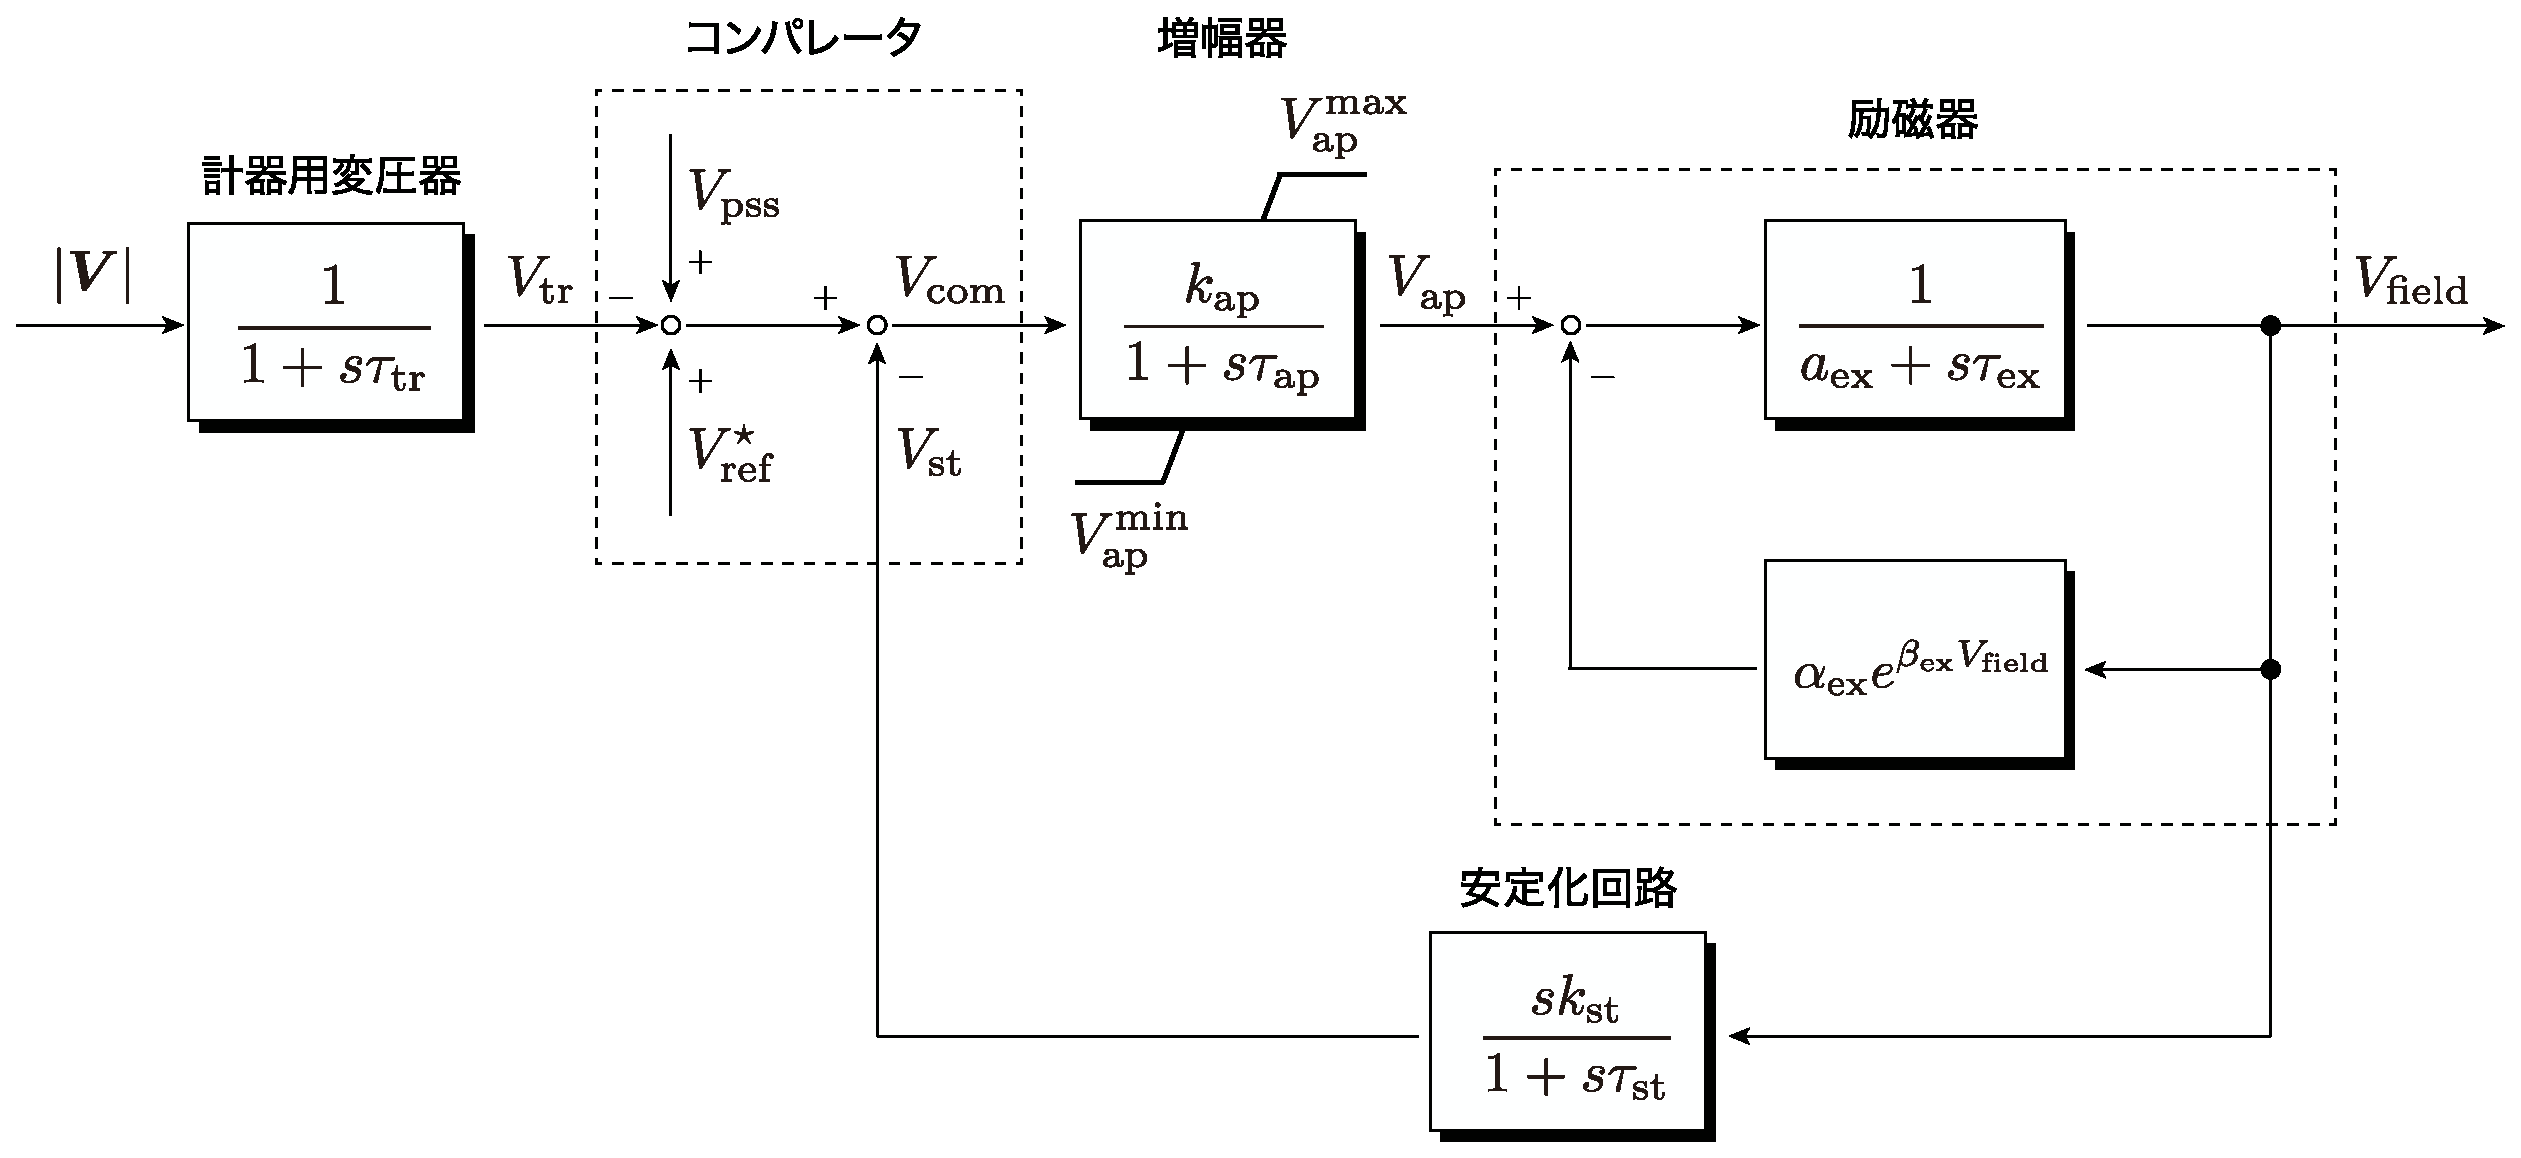
\includegraphics[width = 0.99\linewidth]{figs/avrdc1}
\medskip
\caption{\textbf{自動電圧調整器のIEEE DC1型モデル}}
\label{fig:avrdc1}
\medskip
\end{figure}


\smallskip
\subsubsection{計器用変圧器}

\begin{subequations}\label{eq:stanAVR}
母線電圧を制御回路に使用可能な電圧に降圧させるための機器であり,その動特性は1次遅れフィルタとして
\begin{align}\label{eq:trnsmod}
\tau_{\rm tr} \dot{V}_{\rm tr} = - V_{\rm tr} +  |\bm{V}|
\end{align}
でモデル化される。
一般に,時定数$\tau_{\rm tr}$は十分に小さいため,計器用変圧器の出力$V_{\rm tr}$は母線電圧フェーザの絶対値$|\bm{V}|$とほぼ等しい。

\smallskip
\subsubsection{コンパレータ}

計器用変圧器の出力$V_{\rm tr}$と参照信号$V_{\rm ref}^{\star}$の差分を出力する機器である。
後述する系統安定化装置の出力$V_{\rm pss}$は,定数である$V_{\rm ref}^{\star}$を調整する信号として印加される。
また,励磁系の安定化回路を組み込む場合には,その出力$V_{\rm st}$もフィードバックされる。
すなわち,コンパレータは
\begin{align}\label{eq:compmod}
V_{\rm com} = V_{\rm ref}^{\star} + V_{\rm pss}- V_{\rm tr}
- V_{\rm st}
\end{align}
のようにモデル化される。
上述のように,$V_{\rm tr}$は$|\bm{V}|$とほぼ等しいことから,系統安定化装置の出力$V_{\rm pss}$や安定化回路の出力$V_{\rm tr}$が0であるならば,コンパレータの出力$V_{\rm com}$は,参照信号と母線電圧フェーザの絶対値の差$V_{\rm ref}^{\star} - |\bm{V}|$とほぼ等しい。

\smallskip
\subsubsection{増幅器}

コンパレータの出力$V_{\rm com}$を増幅して励磁器を駆動させるための機器である。回転型や電磁気型などの種類があるが,どの場合にも
\begin{align}\label{eq:ampmod}
\simode{
\tau_{\rm ap} \dot{V}_{\rm ap} & = - V_{\rm ap} + k_{\rm ap} V_{\rm com} \\
V_{\rm ap}^{\rm sat} & = \sfsat(V_{\rm ap};V_{\rm ap}^{\rm min},V_{\rm ap}^{\rm max})
}
\end{align}
でモデル化される。
ただし,時定数$\tau_{\rm ap}$とゲイン$k_{\rm ap}$は非負定数であり,$\sfsat$は
\[
\sfsat(x;\underline{\alpha},\overline{\alpha}) := \left\{
\begin{array}{cl}
\underline{\alpha}, & x \leq \underline{\alpha} \\
x, & \underline{\alpha} < x \leq \overline{\alpha} \\
\overline{\alpha}, & x> \overline{\alpha}
\end{array}
\right.
\]
で定義される飽和関数である。

\smallskip
\subsubsection{励磁器}

増幅器の出力$V_{\rm ap}^{\rm sat}$から界磁電圧$V_{\rm field}$を生成する機器であり,非線形の1次系として
\begin{align}\label{eq:extmod}
\tau_{\rm ex}\dot{V}_{\rm field} =
- \Bigl( 
a_{\rm ex} V_{\rm field} + 
\underbrace{\alpha_{\rm ex} e^{\beta_{\rm ex} V_{\rm field}}}_{\ast} 
\Bigr) 
+V_{\rm ap}^{\rm sat}
\end{align}
でモデル化される。
ただし,$\tau_{\rm ex}$は正の定数であるが,$a_{\rm ex}$は一般に負の定数であることに注意されたい。
また,「$\ast$」で表される項は励磁器内の磁気飽和などの影響による非線形性を表しており,$\alpha_{\rm ex}$と$\beta_{\rm ex}$はともに非負定数である。
通常の動作点の近傍では,励磁器の動特性は安定となるように各定数は設定される。

\smallskip
\subsubsection{安定化回路}

励磁系の安定度を高めるために補助的に実装される回路である。
IEEE DC1型モデルでは,界磁電圧の微分値をフィードバックする機構として表現される。
すなわち,その動特性は
\begin{align}\label{eq:stcmod}
\tau_{\rm st}\dot{V}_{\rm st} =
- V_{\rm st}
+ k_{\rm st} \dot{V}_{\rm field}
\end{align}
で表される。
ただし,時定数$\tau_{\rm st}$とゲイン$k_{\rm st}$は非負定数である。
この安定化回路の出力$V_{\rm st}$は,式\ref{eq:compmod}のコンパレータにフィードバックされる。
\end{subequations}

以上の式\ref{eq:trnsmod}--\ref{eq:stcmod}を統合したものが,自動電圧調整器のIEEE DC1型モデルである。
\ref{table:AVRpara1}と\ref{table:AVRpara2}に各パラメータの参考値をまとめる。
時定数の単位は[s],それ以外の単位は[pu]である。

\begin{table}[h]
\medskip
 \caption{\textbf{IEEE DC1型モデルのパラメータ例}}
 \label{table:AVRpara1}
 \centering
  \begin{tabular}{ccccccc}
   \hline
 &  $\tau_{\rm tr}$ & $\tau_{\rm ap}$ & $k_{\rm ap}$ & $V_{\rm ap}^{\rm max}$ & $V_{\rm ap}^{\rm min}$ \\
   \hline \hline
   例1 \cite[Table D.3. Unit F2]{anderson2008power}& 0.00 & 0.05 & 57.1 & 1.00 & $-1.00$\\
   例2 \cite[8.6.3節]{kundur1994power}& 0.05 & 0.89 & 187 & 1.70 & $ -1.70 $\\
   \hline
  \end{tabular}
\end{table}

\begin{table}[h]
\medskip
 \caption{\textbf{IEEE DC1型モデルのパラメータ例(つづき)}}
 \label{table:AVRpara2}
 \centering
  \begin{tabular}{cccccccc}
   \hline
&    $\tau_{\rm ex}$ & $a_{\rm ex}$ & $\alpha_{\rm ex}$ & $\beta_{\rm ex}$ & $\tau_{\rm st}$ & $k_{\rm st}$\\
   \hline \hline
  例1 \cite[Table D.3. Unit F2]{anderson2008power}& 0.50 & $-0.045$ & 0.0012 & 1.21 & 1.00 & 0.08\\
  例2 \cite[8.6.3節]{kundur1994power}& 1.15 & $-0.30$ & 0.014 & 1.55 & 0.62 & 0.058 \\
   \hline 
  \end{tabular}
\end{table}


%\begin{table}[h]
%\medskip
% \caption{計器用変圧器と増幅器のパラメータ範囲(参考値)}
% \label{table:AVRpara1}
% \centering
%  \begin{tabular}{|c|c|c|c|c|c|}
%   \hline
%   $\tau_{\rm tr}$ & $\tau_{\rm ap}$ & $k_{\rm ap}$ & $V_{\rm ap}^{\rm max}$ & $V_{\rm ap}^{\rm min}$ \\
%   \hline \hline
%   0 -- 0.06 & 0.02 -- 0.25 & 25 -- 400 & 1.0 -- 8.2 & $V_{\rm ap}^{\rm max} \times (-1)$\\
%   \hline
%  \end{tabular}
%\end{table}
%
%\begin{table}[h]
%\medskip
% \caption{励磁器と安定化回路のパラメータ範囲(参考値)}
% \label{table:AVRpara2}
% \centering
%  \begin{tabular}{|c|c|c|c|c|c|}
%   \hline
%    $\tau_{\rm ex}$ & $a_{\rm ex}$ & $\alpha_{\rm ex}$ & $\beta_{\rm ex}$ & $\tau_{\rm st}$ & $k_{\rm st}$\\
%   \hline \hline
%   0.5 -- 1.3 & $-0.17$ -- $-0.05$ & 0.0016 -- 0.011 & 0.79 -- 1.56 & 0.35 -- 1.0 & 0.01 -- 0.08\\
%   \hline
%  \end{tabular}
%\end{table}

\begin{figure}[t]
\centering
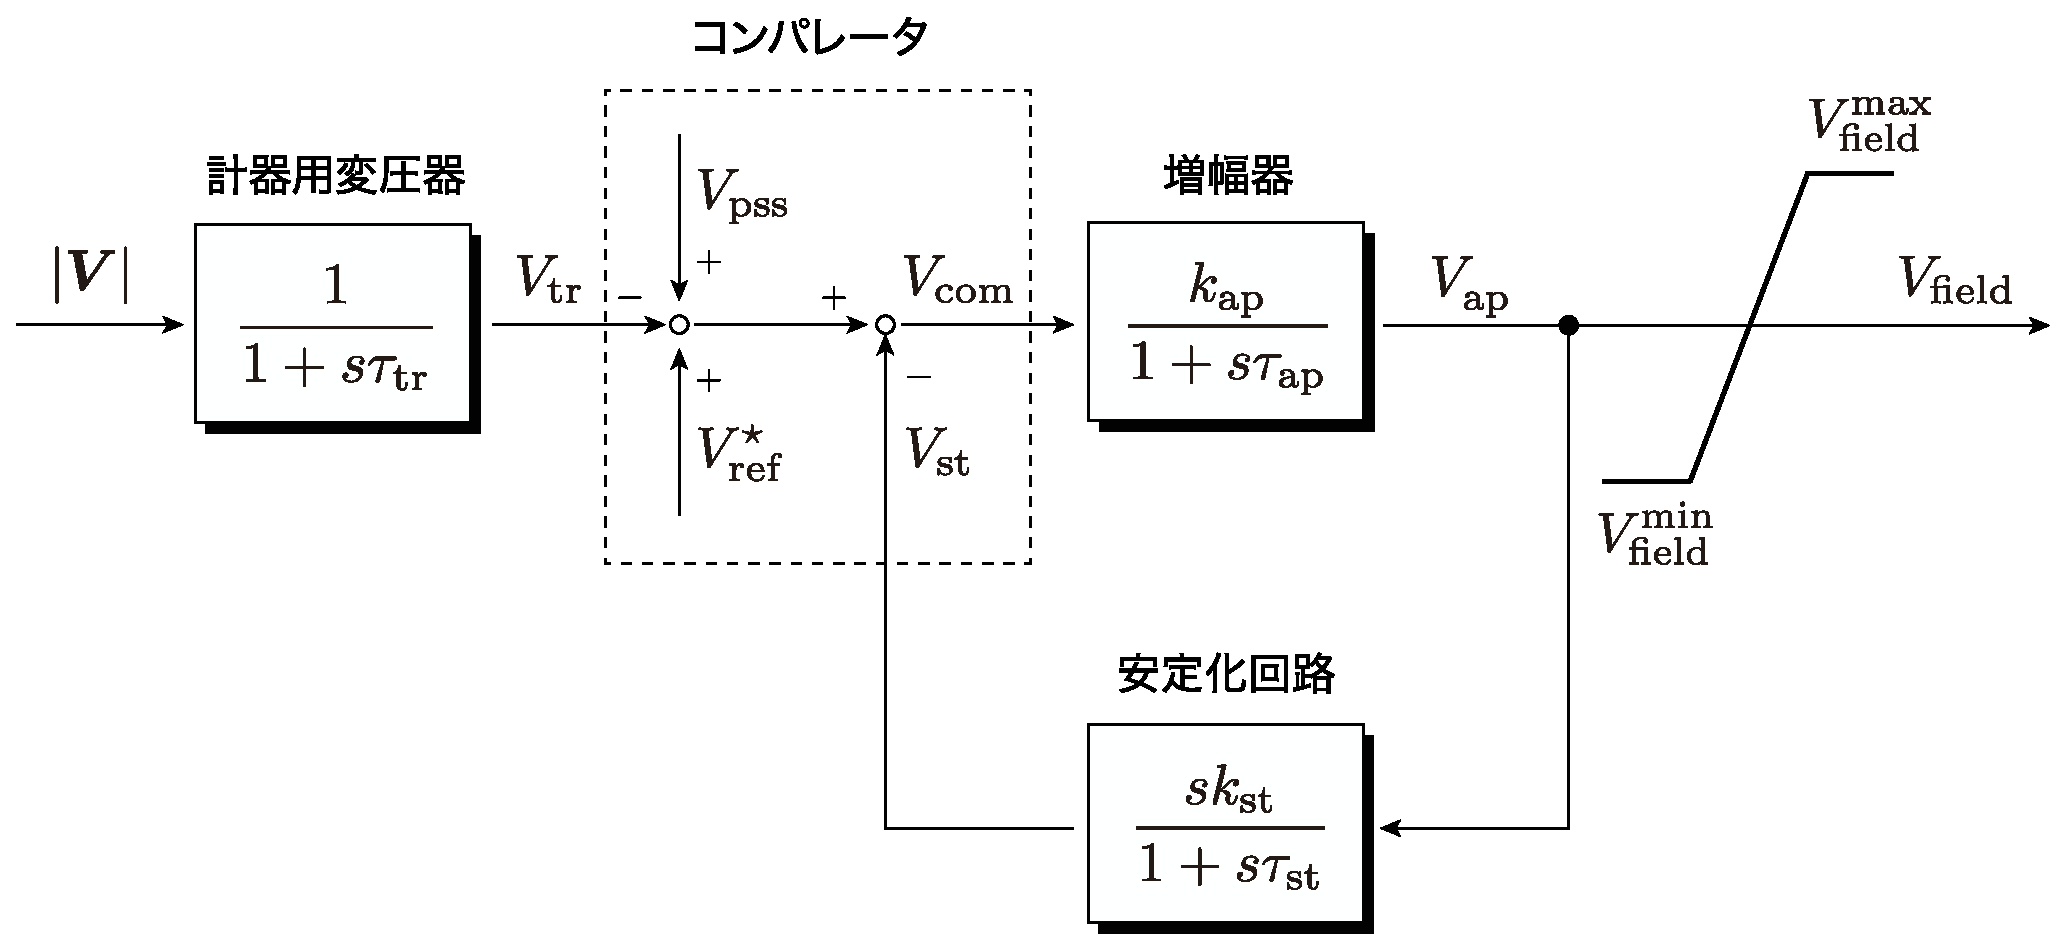
\includegraphics[width = .75\linewidth]{figs/avrst1}
\medskip
\caption{\textbf{自動電圧調整器のIEEE ST1型モデル}}
\label{fig:avrst1}
\medskip
\end{figure}

つぎに,IEEE DC1型と同様の構成であるが,より応答が速い静的型モデルである\textbf{IEEE ST1型モデル}(IEEE Type ST1 excitation system model)を説明する。
この自動電圧調整器モデルでは,励磁器の時定数が十分に小さく,式\ref{eq:extmod}の励磁器モデルが静的な関係として
\[
V_{\rm field} = V_{\rm ap}^{\rm sat}
\]
で表現される。
ただし,式\ref{eq:ampmod}の増幅器における出力飽和の上下限は,主に母線電圧フェーザの絶対値に依存するようにモデル化される\cite[8.63節]{kundur1994power}。
具体的には,$|\bm{V}|$に加えて式\ref{eq:gendifavr}の$E_{\rm field}$を用いて
\[
V_{\rm ap}^{\rm min} = \gamma_{-} |\bm{V}|, \qquad
V_{\rm ap}^{\rm max} = \gamma_{+} |\bm{V}|
-
k_0 E_{\rm field}
\]
とする。
ただし,$\gamma_{-}$,$\gamma_{+}$,$k_{0}$は非負の定数であり,$E_{\rm field}$はpuの単位系では発電機の界磁電流の値と等しい。
このモデルのブロック線図を\FIGref{fig:avrst1}に示す。



IEEE ST1型モデルは励磁器の応答速度が十分に早いため,安定化回路がしばしば取り除かれる。
また,増幅器の時定数$\tau_{\rm ap}$が十分に小さく,その動特性が無視できるとき,簡略化された1次系モデルとして
\begin{align}\label{eq:avrst1}
\simode{
\tau_{\rm tr} \dot{V}_{\rm tr} & = - V_{\rm tr} +  |\bm{V}|  \\
V_{\rm ap} &= k_{\rm ap} ( V_{\rm ref}^{\star} + V_{\rm pss}- V_{\rm tr} )\\
V_{\rm field} & = \sfsat \left(
V_{\rm ap};
V_{\rm ap}^{\rm min},V_{\rm ap}^{\rm max} 
\right)
}
\end{align}
が用いられる。
例えば,このモデルは\cite[12.4節]{kundur1994power}や\cite[4.2.2節]{pal2006robust}などで用いられている。
パラメータ例を\ref{table:AVRparast1}に示す。


\begin{table}[h]
\medskip
 \caption{\textbf{IEEE ST1型モデルのパラメータ例}}
 \label{table:AVRparast1}
 \centering
  \begin{tabular}{ccccccc}
   \hline
 &  $\tau_{\rm tr}$ & $k_{\rm ap}$ & $\gamma_{+}$ & $\gamma_{-}$ & $k_{0}$\\
   \hline \hline
   例1 \cite[8.6.3節]{kundur1994power}& 0.015 & 200 & 7.00 & $-6.40$ & 0.04 \\
   例2 \cite[Table H.23]{ieee2016ieee}& 0.02 & 210 & 6.43 & $-6.00$ & 0.038 \\
   \hline
  \end{tabular}
\end{table}

なお,式\ref{eq:avrst1}の参照信号$V_{{\rm ref}}^{\star}$の値は,所望の界磁電圧の定常値$V_{{\rm field}}^{\star}$と母線電圧の絶対値の定常値$|\bm{V}^{\star}|$が与えられるとき
\begin{align}\label{eq:avrref}
V_{{\rm ref}}^{\star} = \frac{V_{{\rm field}}^{\star}}{k_{{\rm ap}}}+|\bm{V}^{\star}|
\end{align}
と定められる。
ただし,現実の系統運用では,母線電圧や界磁電圧の定常値は負荷の分布などによって変化する未知の値であるため,標準的な母線電圧や界磁電圧の値を用いて参照信号$V_{{\rm ref}}^{\star}$の値を指定する。

\subsection{自動電圧調整器の制御効果}

自動電圧調整器の制御効果を簡単な電力系統モデルを用いて解析してみよう。



\begin{例}[自動電圧調整器による定態安定性と過渡安定度の変化]\label{ex:avreffect}
例\ref{ex:inires}で扱った3母線で構成される電力系統モデルを考えよう。
発電機や送電線の物理定数は例\ref{ex:inires}と同じ値に設定する。
また,母線2に接続されている負荷は定インピーダンスモデルに設定し,そのインピーダンス値には\ref{table:loadpara1}の1行目の値を用いる。
自動電圧調整器は式\ref{eq:avrst1}のIEEE ST1型モデルに設定する。
発電機1と発電機3に組み込まれる自動電圧調整器は同一であり,パラメータは\ref{table:AVRparast1}における例1の値を用いる。

まず,自動電圧調整器の有無に対する定態安定な定常潮流状態(安定な平衡点)の集合の変化を確認する。
具体的には,発電機の内部電圧の定常値である$E_1^{\star}$と$E_3^{\star}$は\ref{table:genst13a}の最右列の値に固定して,回転子偏角の定常値の差である$\delta_1^{\star}-\delta_3^{\star}$をパラメータとして変化させることにより,対応する電力系統の定常潮流状態の定態安定性を近似線形化に基づき判定する
\footnote{
一般性を失うことなく,$\delta_1^{\star}$もしくは$\delta_3^{\star}$を0に設定できる。
また,各発電機の内部状態の定常値を定めれば,対応する機械的トルクや界磁電圧の定常値は
\begin{align*}
\simode{
P_{{\rm mech}i}^{\star} &= %\textstyle
  f_i \left( \delta^{\star},E^{\star} \right)
\\
V_{{\rm field}i}^{\star} & = %\textstyle
   \tfrac{ \Xsi }{\Xti }  E_i^{\star}  - \left(
\Xsi - \Xti
\right)
g_i \left( \delta^{\star},E^{\star} \right)
}
\qquad
 i \in \{1,3\}
\end{align*}
により定められる。
ただし,$\delta^{\star}$と$E^{\star}$は,$\delta_i^{\star}$と$E_i^{\star}$を並べたベクトルであり,関数$f_i$と$g_i$は,式\ref{eq:figidef}で定義される。
さらに,発電機母線の電圧フェーザの定常値は,式\ref{eq:colVi}を用いることにより
\begin{align*}
\mat{
\bm{V}_1^{\star}\\
\bm{V}_3^{\star}
} =
\left(
\mat{
\tfrac{1}{\bm{j} \Xt_1 } & 0\\
0 & \tfrac{1}{\bm{j} \Xt_3 }
} + 
\bm{Y}_{\rm Kron}
\right)^{-1}
\mat{
\tfrac{e^{\bm{j} \delta_1^{\star}}}{\bm{j} \Xt_1 } & 0 \\
0 & \tfrac{e^{\bm{j} \delta_3^{\star}}}{\bm{j} \Xt_3 }
}
\mat{
E_1^{\star}  \\
E_3^{\star} 
}
\end{align*}
として求められる。
ただし,$\bm{Y}_{\rm Kron}$は,\ref{eq:Kron}で定義される負荷母線をクロン縮約したアドミタンス行列である。
なお,参照信号$V_{{\rm ref}i}^{\star}$の値は式\ref{eq:avrref}により定める。
}。
実際に近似線形モデルが安定となる$\delta_1^{\star}-\delta_3^{\star}$の範囲を計算すると,自動電圧調整器なしの場合には\ref{table:stableeqs}の(i)の範囲であり,ありの場合には\ref{table:stableeqs}の(ii)の範囲となることがわかる。
この結果から,自動電圧調整器を組み込むことによって,安定な平衡点の集合は縮小する傾向にあることがわかる。

\begin{table}[h]
\medskip
 \caption{\textbf{定態安定となる回転子偏角の定常値}}
 \label{table:stableeqs}
 \centering
  \begin{tabular}{ccccccccccc}
   \hline
 & (i) AVRなし & (ii) AVRあり & (iii) AVR \& PSSあり \\
   \hline \hline
 $\delta_1^{\star}-\delta_3^{\star}$ の上限~[rad]  & $0.90$ & $0.30$ & $1.10$ \\
 $\delta_1^{\star}-\delta_3^{\star}$ の下限~[rad] & $-1.03$ & $-0.87$ & $-1.32$  \\
   \hline
  \end{tabular}
\end{table}

つぎに,自動電圧調整器によって過渡安定度が向上することを確認する。
具体的には,以下の解析を行う。
まず,自動電圧調整器の有無に依らず定態安定な定常潮流状態として,回転子偏角差の定常値が$\delta_1^{\star}-\delta_3^{\star}$が$\tfrac{\pi}{6}$~[rad]である場合を考える。
ただし,内部電圧の定常値は上記の値に設定する。
つぎに,電力系統モデルの初期値をパラメータとして変化させて,得られた周波数偏差の時間応答について$\|\Delta\omega\|_{\mathcal{L}_2}$を計算する。
ただし,$\Delta \omega$は$\Delta \omega_1$と$\Delta \omega_3$を並べたベクトルである。
同様に,母線電圧フェーザの時間応答について$\||\bm{V}|-|\bm{V}^{\star}| \|_{\mathcal{L}_2}$を計算する。
ただし,$|\bm{V}|$は$|\bm{V}_1|$と$|\bm{V}_3|$を並べたベクトルであり,$|\bm{V}^{\star}|$は$|\bm{V}_1^{\star}|$と$|\bm{V}_3^{\star}|$を並べたベクトルである
\footnote{
注目する平衡点の安定領域の内側に初期値を与える場合には,周波数偏差や母線電圧フェーザ偏差などの$\mathcal{L}_2$ノルムの値は有限となる。
また,それらの$\mathcal{L}_2$ノルムの値が小さいほど,与えた初期値に対する平衡点の過渡安定度が高いことがわかる。
一方で,安定領域の外側に初期値を与える場合には,$\mathcal{L}_2$ノルムの値は無限大となる。
}。

過渡安定度の解析結果を\FIGref{fig:transientL2}に示す。
横軸は設定した$\delta_1-\delta_3$の初期値を表しており,縦軸は設定された初期値において生じた周波数偏差や母線電圧フェーザ偏差の$\mathcal{L}_2$ノルムの値を表している。
青の実線が自動電圧調整器なしの場合,赤の破線が自動電圧調整器ありの場合に対応しており,$\mathcal{L}_2$ノルムの値が有限である初期値の範囲でそれぞれプロットされている。
なお,内部電圧$E_1$,$E_3$の初期値は,それらの定常値$E_1^{\star}$,$E_3^{\star}$と同じ値に設定している。
また,周波数偏差$\Delta \omega_1$,$\Delta \omega_3$の初期値はどちらも0に設定している。
この結果から,自動電圧調整器を組み込むことによって,周波数偏差で評価する場合の過渡安定度が向上していることがわかる。
また,自動電圧調整器の有無によって安定領域の大きさにはほとんど変化がないこともわかる。

参考として,$\delta_1-\delta_3$の初期値を$-1$に設定した場合と,$-1.57$に設定した場合に生じる周波数偏差の時間応答をそれぞれ,\FIGref{fig:avrsmalld}と\FIGref{fig:avrlarged}に示す。
(a)が自動電圧調整器なしの場合であり,(b)が自動電圧調整器ありの場合である。
この結果から,自動電圧調整器を組み込むことによって,周波数偏差の振動の低周波成分(振動の中心値)がより速く0に収束する傾向がわかる。
一方で,自動電圧調整器の有無に関わらず,振動の高周波成分の減衰率には大きな変化がないこともわかる。
\end{例}



%\begin{figure}[t]
%\centering
%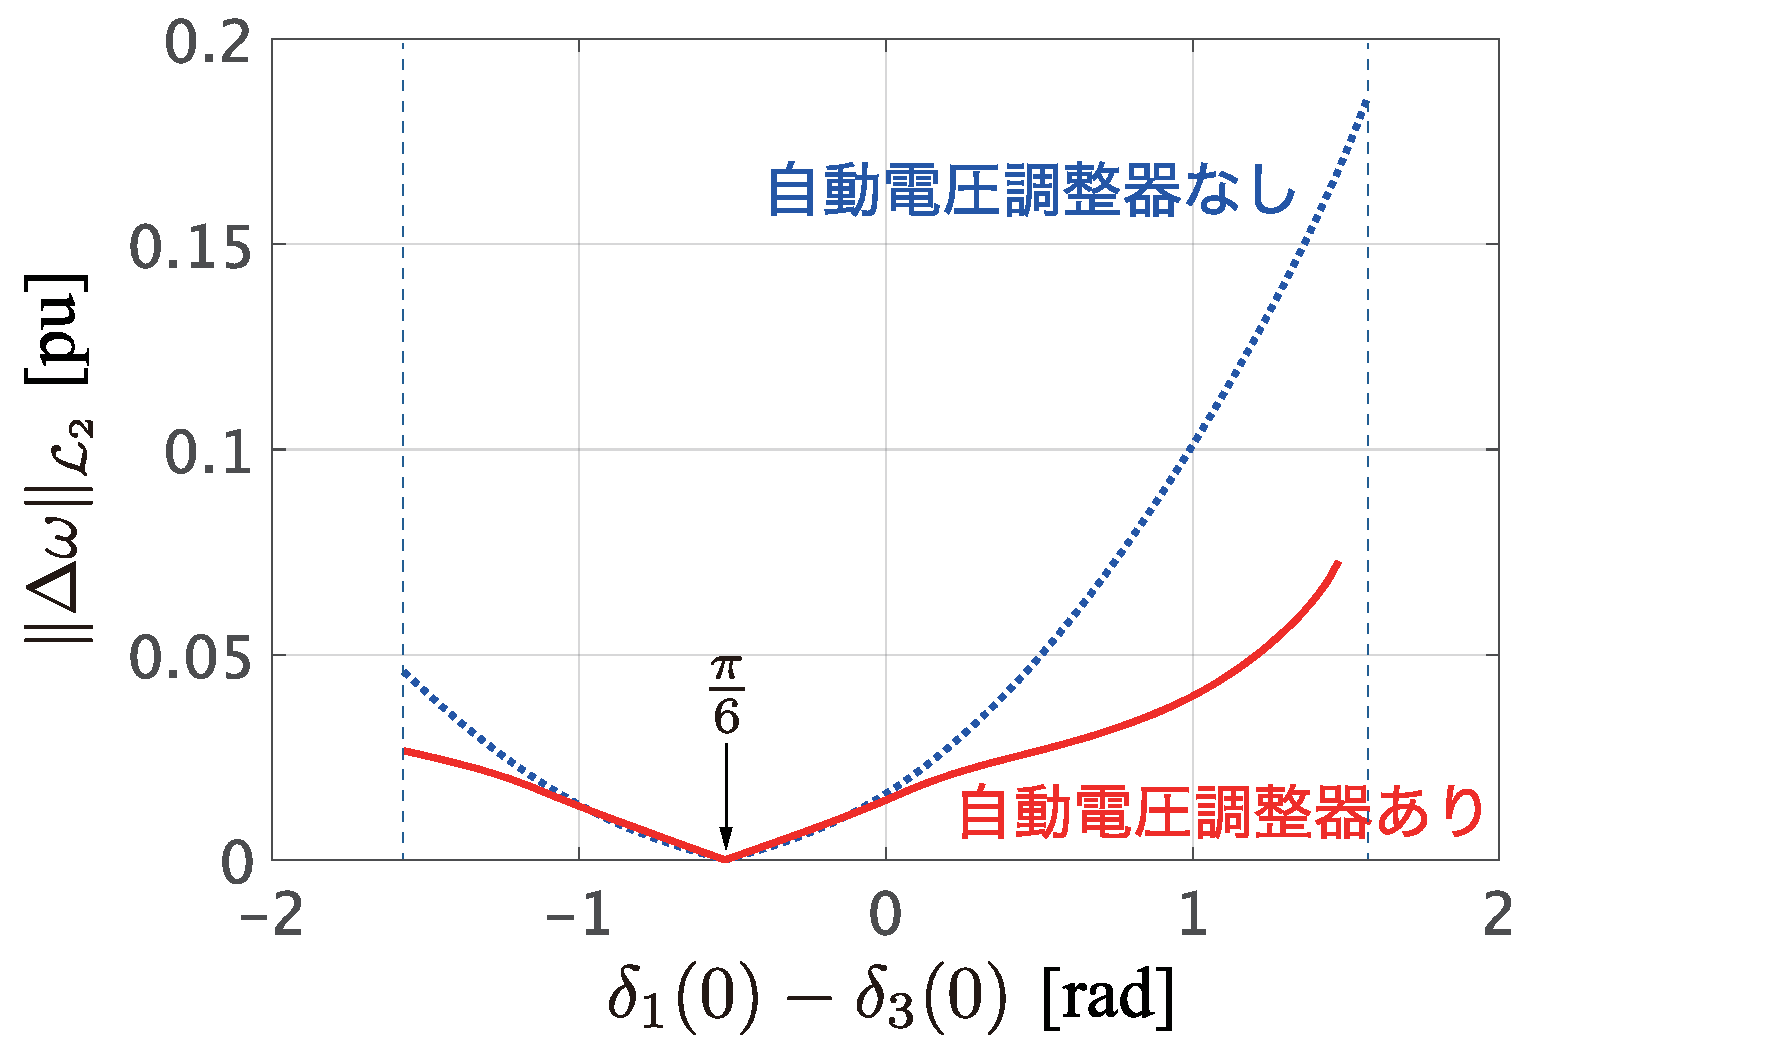
\includegraphics[width = .65\linewidth]{figs/transientL2}
%\medskip
%\caption{\textbf{ 自動電圧調整器による過渡安定度の変化} }
%\label{fig:transientL2}
%\medskip
%\end{figure}

\begin{figure}[t]
  \centering
  {
  \begin{minipage}{0.49\linewidth}
    \centering
    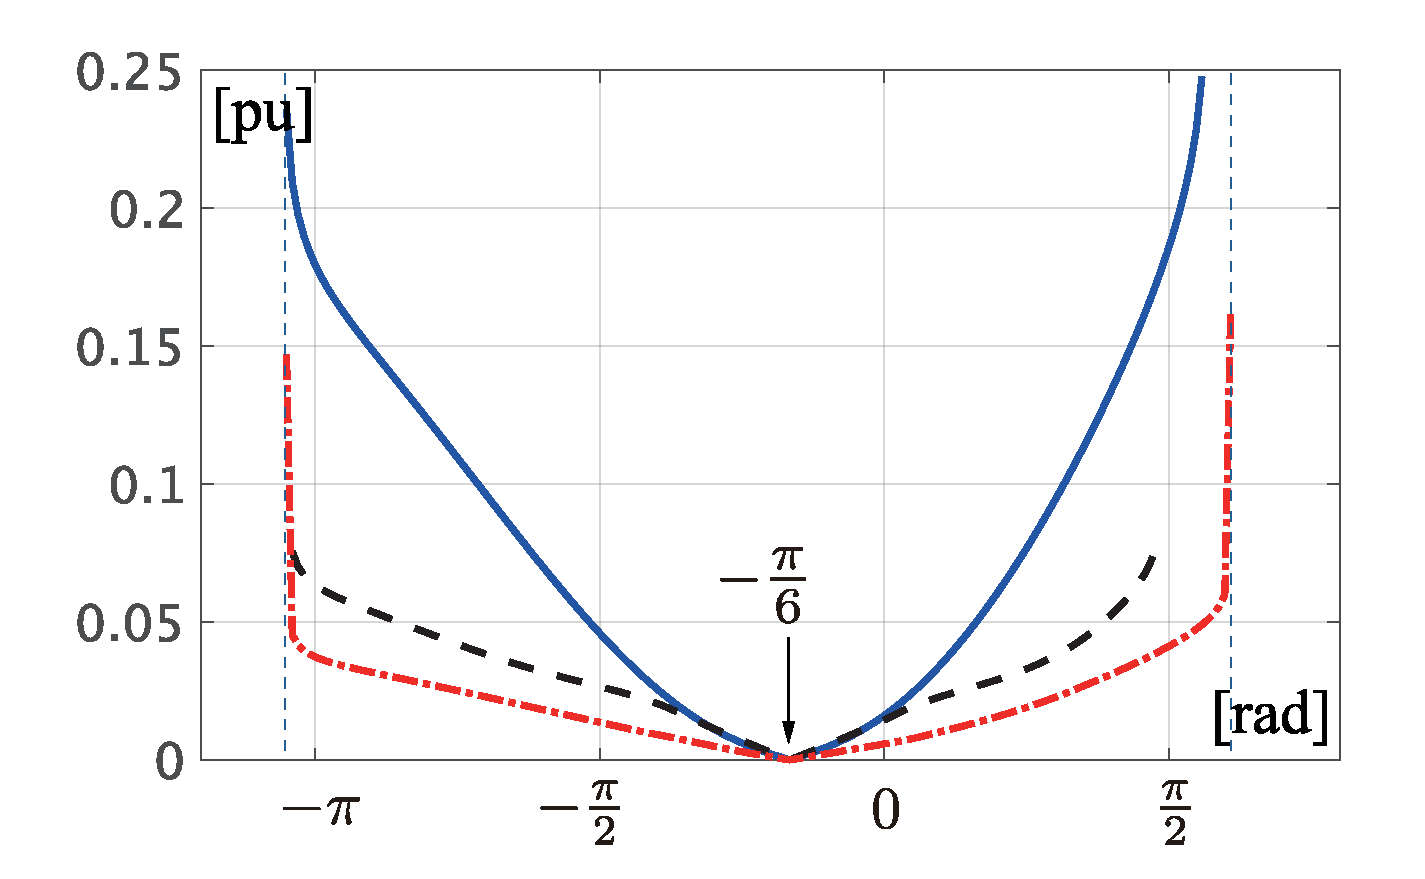
\includegraphics[width = 1.0\linewidth]{figs/transientL2w}
    \subcaption{ $\|\Delta\omega\|_{\mathcal{L}_2}$}
  \end{minipage}
  \begin{minipage}{0.49\linewidth}
    \centering
    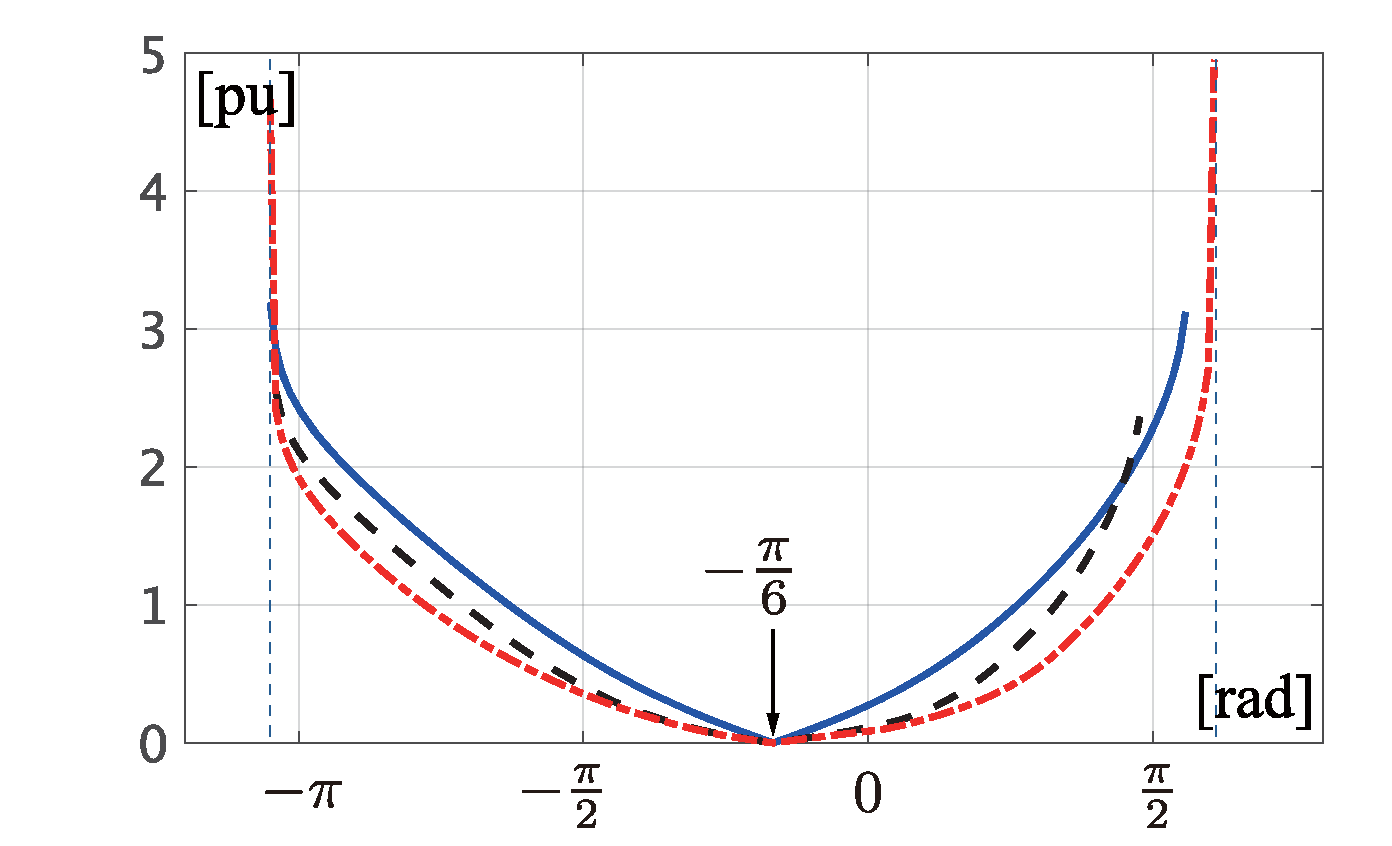
\includegraphics[width = 1.0\linewidth]{figs/transientL2V}
    \subcaption{ $\||\bm{V}|-|\bm{V}^{\star}| \|_{\mathcal{L}_2}$ }
  \end{minipage}
  \medskip
  \caption{\textbf{自動電圧調整器による過渡安定度の変化} }
  \label{fig:transientL2}
  }
\medskip
\end{figure}



\begin{figure}[t]
  \centering
  {
  \begin{minipage}{0.49\linewidth}
    \centering
    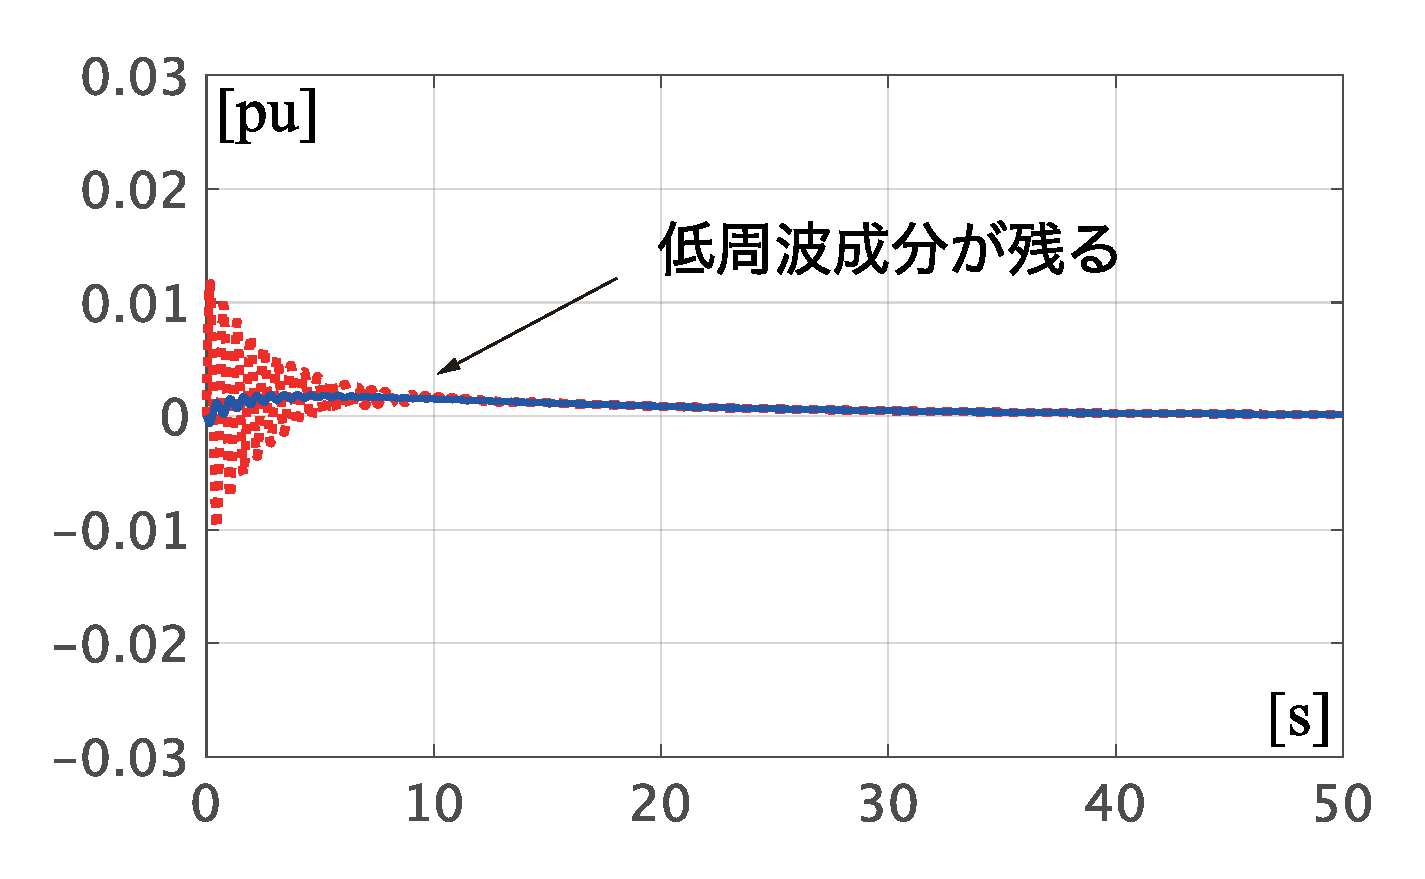
\includegraphics[width = 1.0\linewidth]{figs/woAVRsmall}
    \subcaption{ 自動電圧調整器なし}
  \end{minipage}
  \begin{minipage}{0.49\linewidth}
    \centering
    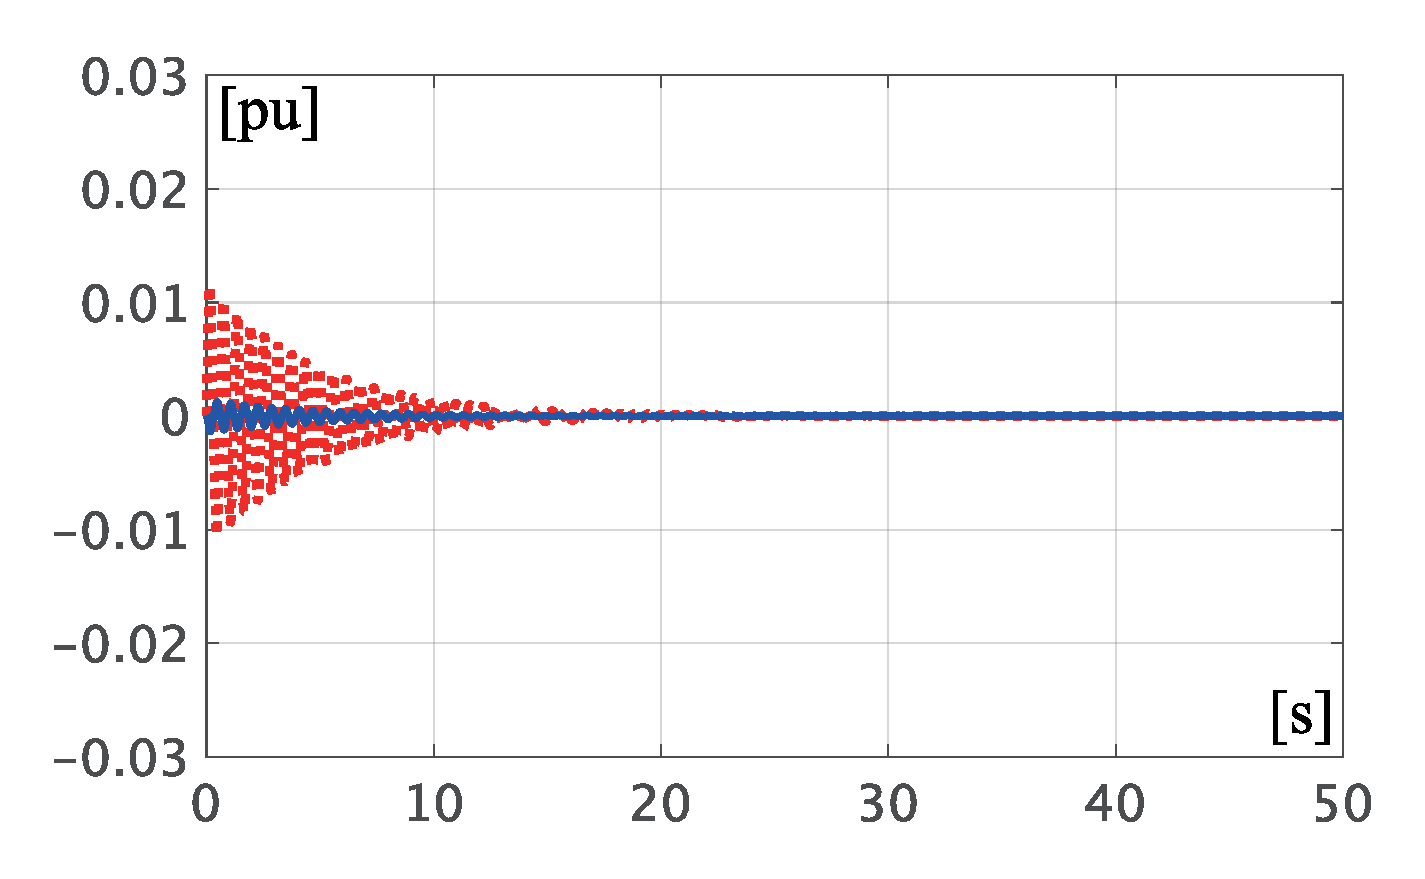
\includegraphics[width = 1.0\linewidth]{figs/wAVRsmall}
    \subcaption{ 自動電圧調整器あり }
  \end{minipage}
  \medskip
  \caption{\textbf{周波数偏差の時間応答}
  \\ \centering{($\delta_1(0) - \delta_3(0) =-1$の場合)} }
  \label{fig:avrsmalld}
  }
\medskip
\end{figure}

\begin{figure}[t]
  \centering
  {
  \begin{minipage}{0.49\linewidth}
    \centering
    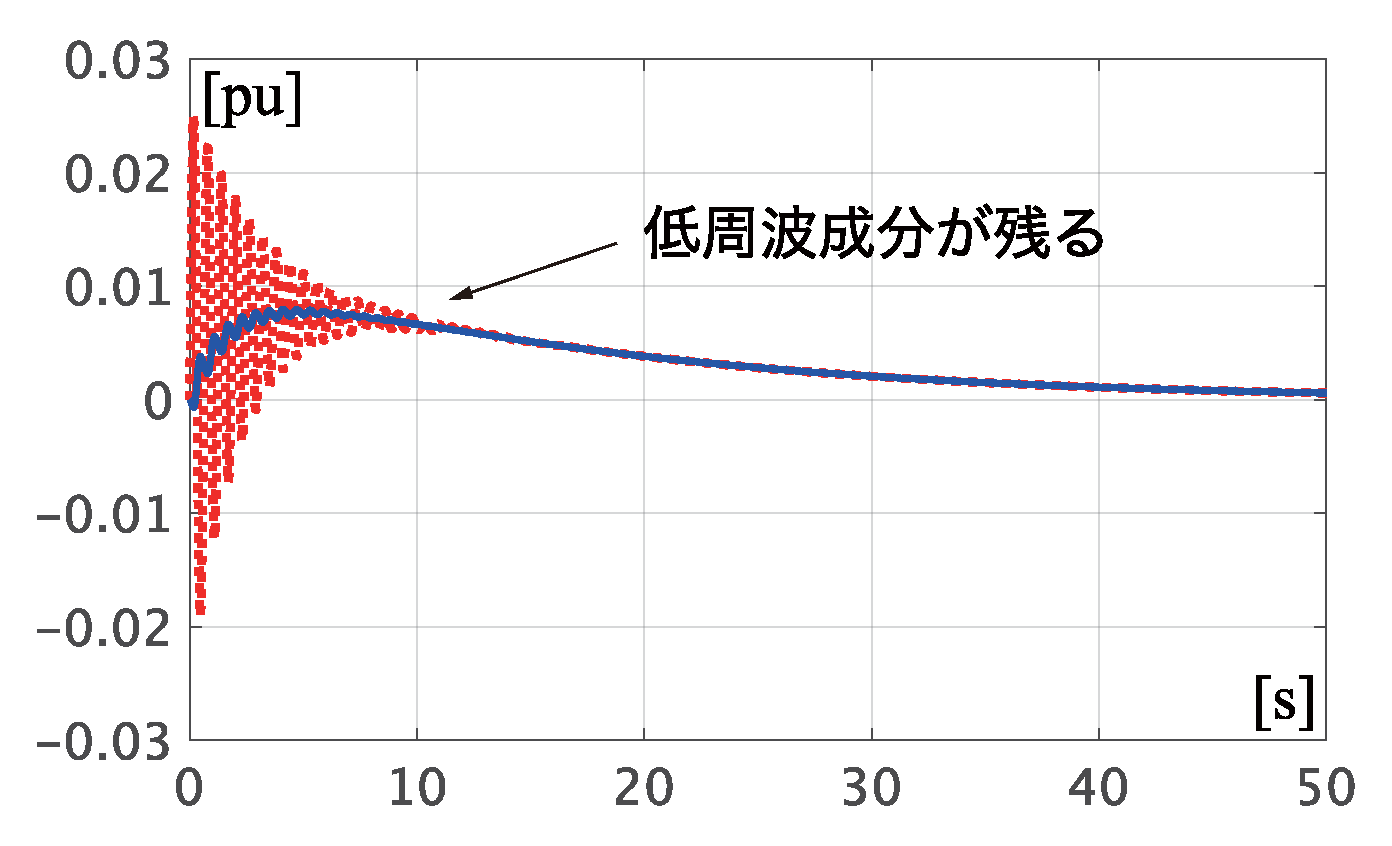
\includegraphics[width = 1.0\linewidth]{figs/woAVRlarge}
    \subcaption{ 自動電圧調整器なし}
  \end{minipage}
  \begin{minipage}{0.49\linewidth}
    \centering
    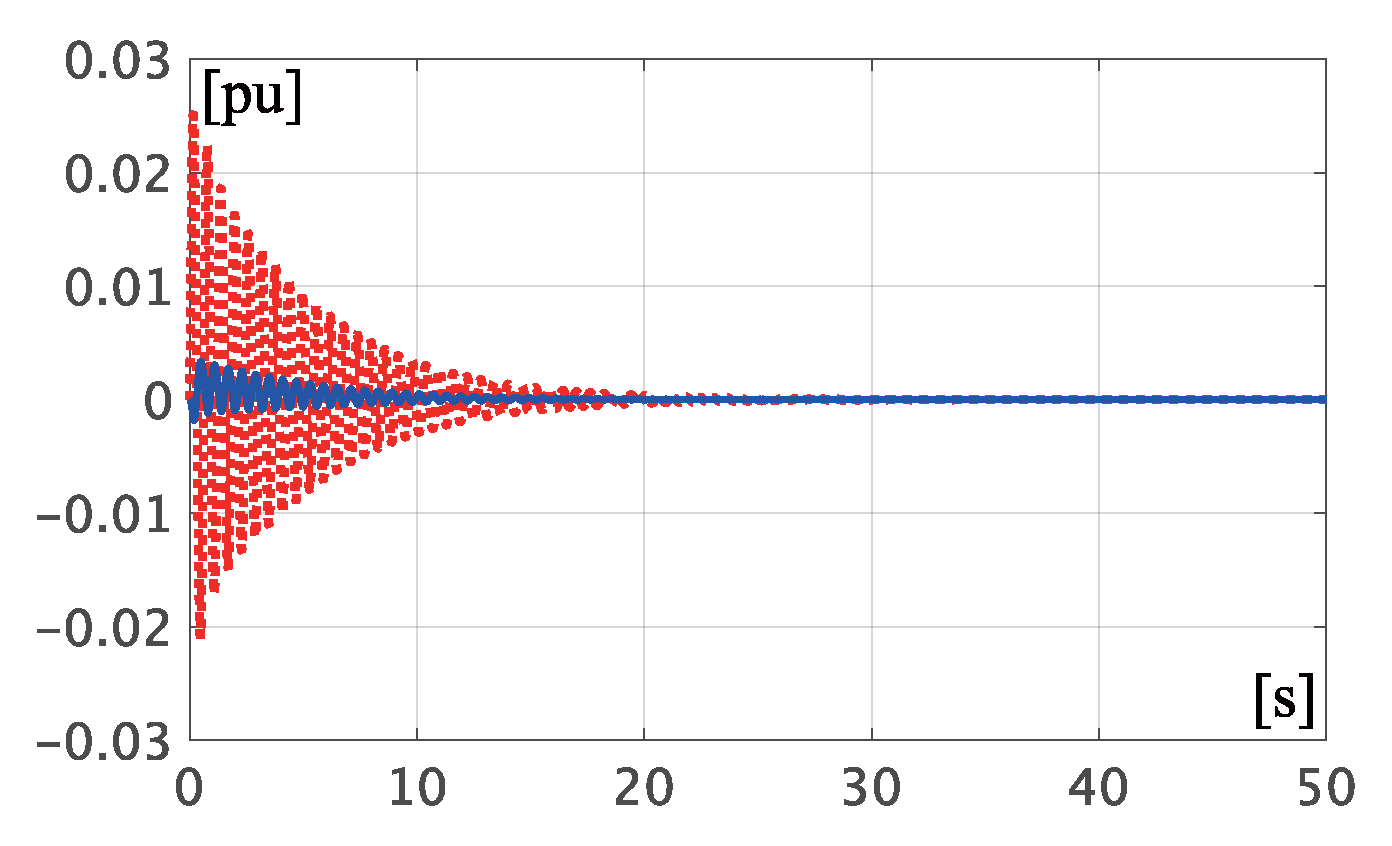
\includegraphics[width = 1.0\linewidth]{figs/wAVRlarge}
    \subcaption{ 自動電圧調整器あり}
  \end{minipage}
  \medskip
  \caption{\textbf{周波数偏差の時間応答}
  \\ \centering{($\delta_1(0) - \delta_3(0) =-1.57$の場合)} }
  \label{fig:avrlarged}
  }
\medskip
\end{figure}



例\ref{ex:avreffect}から,自動電圧調整器を組み込むことによって,実装前に安定であった平衡点の一部が不安定化する傾向にある一方で,周波数偏差の振動における低周波成分が抑制されることがわかる。
この意味で,電力系統の過渡安定度が向上している。
次節で説明する系統安定化装置は,自動電圧調整器では抑制できなかった振動の高周波成分を抑制する効果をもつ。



\subsection{系統安定化装置}

系統安定化装置は\FIGref{fig:avrdc1}や\FIGref{fig:avrst1}に示される追加的な制御信号$V_{\rm pss}$を出力する機器である。
一般に,発電機の周波数偏差や有効電力,母線電圧フェーザなどを計測して系統安定化装置にフィードバックすることが多い。
以下では,\textbf{IEEE PSS1型モデル}(IEEE Type PSS1 power system stabilizer model)と呼ばれる標準的な系統安定化装置のモデルを説明する\cite[9.2節]{ieee2016ieee}。
このモデルは主に,\textbf{ウォッシュアウトフィルタ}(washout filter)と\textbf{位相進み補償器}(phase-lead compensator)の2つで構成される。
ブロック線図を\FIGref{fig:pss1}に示す。

\begin{figure}[t]
\centering
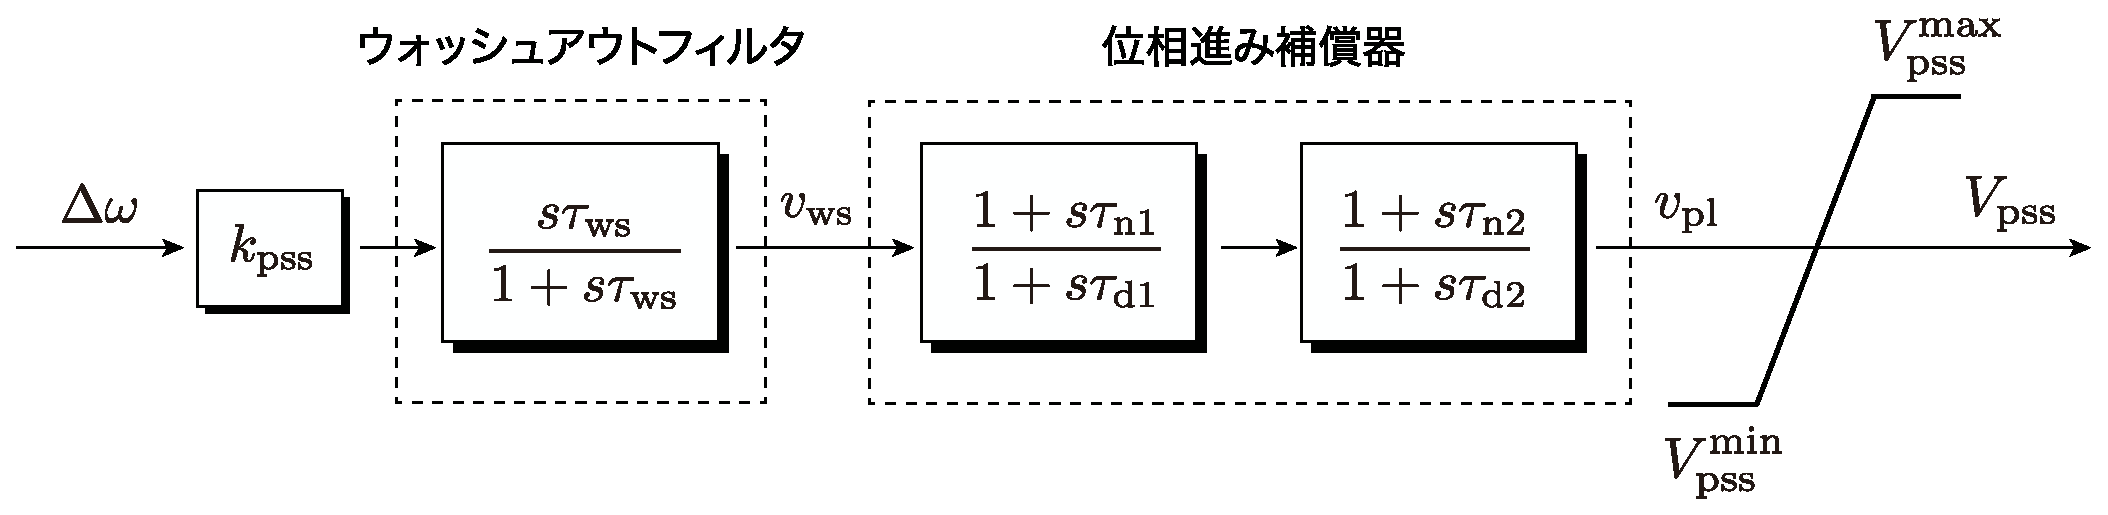
\includegraphics[width = .99\linewidth]{figs/pss1}
\medskip
\caption{\textbf{系統安定化装置のIEEE PSS1型モデル}}
\label{fig:pss1}
\medskip
\end{figure}


\smallskip
\subsubsection{ウォッシュアウトフィルタ}


系統安定化装置の定常ゲインを0とするためのハイパスフィルタであり,ゲイン$k_{\rm pss}$で定数倍された発電機の周波数偏差$\Delta \omega$を入力として,その動特性は
\begin{subequations}\label{eq:pss1mod}
\begin{align}\label{eq:washmod}
\simode{
\tau_{\rm ws} \dot{\xi}_{\rm ws} &=
- \xi_{\rm ws}
+ k_{\rm pss} \Delta \omega \\
v_{\rm ws} &= k_{\rm pss} \Delta \omega - \xi_{\rm ws}
}
\end{align}
で表される。
明らかに,$\Delta \omega$が定数であるならば,ウォッシュアウトフィルタの定常状態での出力$v_{\rm ws}^{\star}$は0となる。
このフィルタの役割は,過渡状態にある電力系統の周波数偏差を抽出することである。
したがって,時定数$\tau_{\rm ws}$は,周波数偏差の整定時間を考慮して,1から20~[s]程度の範囲で設定されることが多い\cite[12.5節]{kundur1994power}。

\smallskip
\subsubsection{位相進み補償器}
母線電圧フェーザから発電機の有効電力までの位相遅れを緩和するために組み込まれる補償器である。
所望の位相進みを実現するために,1から2個程度の位相進み補償器が直列結合されることが多い。
具体的には,ウォッシュアウトフィルタの出力$v_{\rm ws}$を入力として,その動特性は
\begin{align}\label{eq:phldmod}
\simode{
\tau_{{\rm d}1} \dot{\xi}_{1} &=
- \xi_{1}
+ \left( 
1- \tfrac{\tau_{{\rm d}1}}{\tau_{{\rm n}1}}
\right)
v_{\rm ws} \\
v_{1} &= \tfrac{\tau_{{\rm n}1}}{\tau_{{\rm d}1}} (v_{\rm ws} - \xi_{1} )
}
\qquad
\simode{
\tau_{{\rm d}2} \dot{\xi}_{2} &=
- \xi_{2}
+ \left( 
1- \tfrac{\tau_{{\rm d}2}}{\tau_{{\rm n}2}}
\right)
v_{1} \\
v_{\rm pl} &= \tfrac{\tau_{{\rm n}2}}{\tau_{{\rm d}2}} (v_{1} - \xi_{2} )
}
\end{align}
で表される。
%ただし,時定数は$\tau_{{\rm d}1} \leq \tau_{{\rm n}1}$,$\tau_{{\rm d}2} \leq \tau_{{\rm n}2}$となるように設定される。
さいごに,位相進み補償器の出力$v_{\rm pl}$を飽和関数に作用させて
\begin{align}\label{eq:psssat}
V_{\rm pss} = \sfsat \left(
v_{\rm pl};
V_{\rm pss}^{\rm min},V_{\rm pss}^{\rm max} 
\right)
\end{align}
\end{subequations}
とすることで系統安定化装置の出力が得られる。
このモデルのパラメータ例を\ref{table:psspara}に示す。
ただし,系統安定化装置のパラメータは,各発電機の動特性,自動電圧調整器の動特性,負荷の分布,送電網の特性など様々な要素を考慮して決定する必要があるため,例示されたパラメータ設定によって,必ずしも所望の系統安定度が実現されるとは限らないことに注意されたい。
また,標準的な系統安定化装置のパラメータ設計指針は,\ref{sec:onemachine}節で説明された1機無限大母線系統モデルに基づくものが多く,複数の発電機を結合した場合の結果は明らかでないことにも注意が必要である。
例えば,文献\cite[12.5節]{kundur1994power}では,1機無限大母線系統モデルを用いて,古典制御理論に基づくパラメータの設計指針が示されている。
文献\cite{chow2004power}では,現代制御理論に基づく設計指針も解説されている。


\begin{table}[h]
\medskip
 \caption{\textbf{IEEE PSS1型モデルのパラメータ例}}
 \label{table:psspara}
 \centering
  \begin{tabular}{cccccccccccccc}
   \hline
 &  $k_{\rm pss}$ & $\tau_{\rm ws}$ & $\tau_{{\rm d}1}$ & $\tau_{{\rm n}1}$ & $\tau_{{\rm d}2}$ & $\tau_{{\rm n}2}$ & $V_{\rm pss}^{\rm min}$ & $V_{\rm pss}^{\rm min}$ \\
   \hline \hline
   例1 \cite[12.5節]{kundur1994power}& 9.50 & 1.4 & 0.033 & 0.154 & 0.00 & 0.00 & $-\infty$ & $\infty$ \\
   例2 \cite[12.8節]{kundur1994power}& 20.0 & 10.0 & 0.02 & 0.05 & 5.40 & 3.00 & $-\infty$ & $\infty$ \\
   例3 \cite[Table H.3]{ieee2016ieee}& 3.15 & 10.0 & 0.01 & 0.76 & 0.01 & 0.76 & $-0.09$ & 0.09\\
   \hline
  \end{tabular}
\end{table}




\subsection{系統安定化装置の制御効果}\label{sec:pssov}

\begin{例}[xxx]\label{ex:psseffect}
\red{PSSの効果をシステム理論的に説明したい。3バスの例?}
\end{例}


\section{レトロフィット制御理論に基づく系統安定化装置\advanced}\label{sec:retrofit}

\subsection{系統安定化装置の設計に用いる電力系統モデル\advanced}

\smallskip
\subsubsection{レトロフィット制御理論に基づく系統安定化装置の特長}

本節では,レトロフィット制御理論に基づく系統安定化装置の設計手法を説明する\cite{ishizaki2018retrofit,sadamoto2018retrofit,sasahara2019damping,ishizaki2019retrofit,ishizaki2021modularity}。
本手法により設計された系統安定化装置は,複数の発電機に同時並行で組み込む場合にも,電力系統全体を安定に維持することが可能である。
特に,各々の系統安定化装置は
\begin{itemize}
\item それらを組み込む発電機や自動電圧調整器の数理モデルのみを用いて分散設計が可能である
\item 発電機母線の電圧フェーザや電流フェーザなどの局所的な計測信号のみを用いて分散実装が可能である
\end{itemize}
という特長をもつ。
以下では,式\ref{eq:gendifavr}の発電機モデルに対して,式\ref{eq:avrst1}のIEEE ST1型の自動電圧調整器モデルが組み込まれている場合を考える。
ただし,説明の簡単化のため,自動電圧調整器の出力飽和は無視する。
なお,出力飽和がある場合だけでなく,他の形式の自動電圧調整器を組み込む場合や,より詳細な発電機モデルを用いる場合などにおいても同様の議論が可能である。


\smallskip
\subsubsection{局所線形サブシステム}

相互作用入力の設定を工夫することにより,注目する発電機に自動電圧調整器を結合したサブシステムを線形系の形式として
\begin{align}\label{eq:desmodl}
G:\simode{
\dot{x} &= Ax + Bu + Lv \\
w &= \mathit{\Gamma} x \\
y &= Cx
}
\end{align}
で表すことを考える。
ここで,状態$x$は発電機モデルの状態$\delta$,$\Delta \omega$,$E$と自動電圧調整器モデルの状態$V_{\rm tr}$を順に並べたベクトルである。
また,入力$u$は系統安定化装置の出力$V_{\rm pss}$を表し,相互作用の入出力である$v$と$w$は
\begin{align}\label{eq:sigintvw}
v:=
\mat{
P_{\rm mech} - \tfrac{E |\bm{V} |}{ \Xt } \sfsin(\delta -  \angle \bm{V}) \\
k_{\rm ap} V_{\rm ref}^{\star} + 
\left(
\tfrac{ \Xs }{ \Xt }-1
\right)
|\bm{V}| \sfcos (\delta - \angle \bm{V} )\\
|\bm{V}|
}
,\qquad
w:=\mat{
\delta \\
\Delta \omega \\
E 
}
\end{align}
と定義する。
式\ref{eq:sigintvw}の相互作用入力$v$に発電機の非線形項や母線電圧フェーザの変数が含まれていることに注意されたい。
これらの信号の定義に合わせて,式\ref{eq:desmodl}のシステム行列は
\begin{align}\label{eq:matlocalm}
\spliteq{
A&:=\mat{
0 & \omega_0 & 0 & 0 \\
0 & -\tfrac{D}{M} & 0 & 0 \\
0 & 0 & -\tfrac{ \Xs }{ \taud \Xt } & -\tfrac{k_{\rm ap}}{ \taud } \\
0 & 0 & 0 & -\tfrac{1}{\tau_{\rm tr}}
}, \quad
B:=
\mat{
0 \\
0 \\
\tfrac{k_{\rm ap}}{ \taud } \\
0 
},\quad
C= I \\
L &:=
\mat{
0 & 0 & 0 \\
\tfrac{1}{M} & 0 & 0 \\
0 & \tfrac{1}{ \taud } & 0 \\
0 & 0 & \tfrac{1}{\tau_{\rm tr} }
}, \quad
\mathit{\Gamma} :=
\mat{
1 & 0 & 0 & 0 \\
0 & 1 & 0 & 0 \\
0 & 0 & 1 & 0 
}
}
\end{align}
と定義される。
式\ref{eq:desmodl}の$G$を\textbf{局所線形サブシステム}(local linear subsystem)と呼ぶ。
なお,式\ref{eq:matlocalm}のシステム行列のパラメータ,すなわち,局所線形サブシステムのモデルパラメータは既知であり,系統安定化装置の設計や実装に利用可能であるものと仮定する。

\smallskip
\subsubsection{環境と近似線形環境モデル}

出力$y$と相互作用の入出力$v$,$w$が計測可能であるという前提のもとで,系統安定化装置を表す局所コントローラ
\[
K : (y,v,w)\mapsto u
\]
を設計することを考えよう。
%ただし,式\ref{eq:desmodl}の局所線形サブシステム$G$では,出力$w$は出力$y$に包含されることに注意されたい。
以下では,このコントローラ$K$を\textbf{レトロフィットコントローラ}(retrofit controller)と呼ぶ\footnote{
レトロフィット(retrofit)はretroactive とrefitに由来する単語であり,既存のシステムなどに対して部分的な増築や改築を行うことを意味する。
}。
レトロフィットコントローラの設計と実装には,局所線形サブシステム$G$のモデルだけでなく,相互作用出力$w$の情報から相互作用入力$v$を内部的に推定する役割をもつ線形モデルも用いる。
以下では,この推定用モデルを\textbf{近似線形環境モデル}(approximate linear environment model)と呼ぶ。

\begin{figure}[t]
\centering
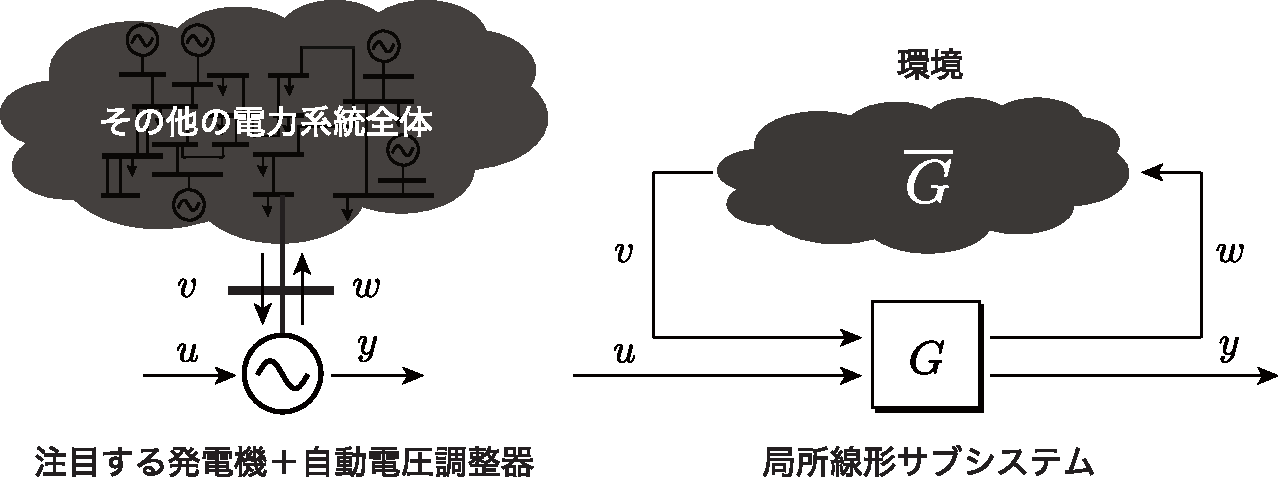
\includegraphics[width = .99\linewidth]{figs/retconsys2}
\medskip
\caption{\textbf{局所サブシステムと環境のフィードバック結合系}}
\label{fig:retconsys}
\medskip
\end{figure}


近似線形環境モデルを説明する準備として,\textbf{環境}(environment)と呼ばれる非線形サブシステムを導入する。
環境は「局所線形サブシステムを除いたシステム全体」を表すサブシステムであり,局所線形サブシステムの相互作用出力$w$を入力とし,相互作用入力$v$を出力とする非線形系である。
形式的に,環境の動的な入出力関係を
\[
\overline{G} : w\mapsto v
\]
と表そう。
このとき,局所線形サブシステム$G$と環境$\overline{G}$のフィードバック結合系は,\FIGref{fig:retconsys}のように注目する発電機の視点からみた電力系統全体を表す。

環境$\overline{G}$には,送電網,負荷,他の発電機などの多数の要素を含むため,注目する発電機に対する系統安定化装置の設計や実装に,環境の完全な非線形モデルが利用可能であると仮定することは現実的ではない。
この事実を考慮して,「環境の近似的な線形モデルのみ」が利用可能である状況を想定しよう。
以下では,説明の簡単化のため,近似線形環境モデルを静的な入出力関係で表すことを考える\footnote{
動的な近似線形環境モデルを用いることも可能である。
詳細は,\cite{ishizaki2019retrofit}を参照されたい。
}。
具体的には,注目する定常潮流状態における相互作用入出力の定常値を$(v^{\star},w^{\star})$と表すとき,近似線形環境モデルを
\begin{align}\label{eq:Gbapxst}
\overline{G}_{\rm apx}:
v_{\rm apx} = v^{\star} + \overline{\mathit{\Theta}} \left(w-w^{\star}\right)
%+ \overline{v}
\end{align}
とパラメータ化する。
ここで,$\overline{\mathit{\Theta}}$はモデルのパラメータを表す行列である。
式\ref{eq:Gbapxst}の近似線形環境モデル$\overline{G}_{\rm apx}$は,相互作用出力$w$が相互作用入力$v$に及ぼす影響を,それらの定常値$(v^{\star},w^{\star})$の近傍における線形予測により推定した値$v_{\rm apx}$を生成する。
レトロフィットコントローラの設計に用いる電力系統モデルは,\FIGref{fig:explocalG}のように,
この近似線形環境モデルのパラメータ$\overline{\mathit{\Theta}}$と局所線形サブシステムのモデルをフィードバック結合して構成する。
具体的には
\begin{align}\label{eq:Gplus}
G_+: \simode{
\dot{\hat{\xi}} &=  \left( A+L \overline{\mathit{\Theta}} 
\mathit{\Gamma} \right) \hat{\xi} + B \hat{u} \\
\hat{y} & = C \hat{\xi}
}
\end{align}
である。
%ただし,システム行列は
%\[
%A_+ :=
%A+L \overline{\mathit{\Theta}} 
%\mathit{\Gamma}
%,\qquad
%B_+ := B
%,\qquad
%C_+ := C
%\]
%である。
ただし,$\hat{u}$,$\hat{y}$は制御系設計用の仮想的な入出力信号であるため,ハット記号をつけて$u$,$y$と区別した。
なお,式\ref{eq:matlocalm}において$C$は単位行列であることから,出力$\hat{y}$は$G_+$の内部状態$\hat{\xi}$に等しい。

\begin{figure}[t]
\centering
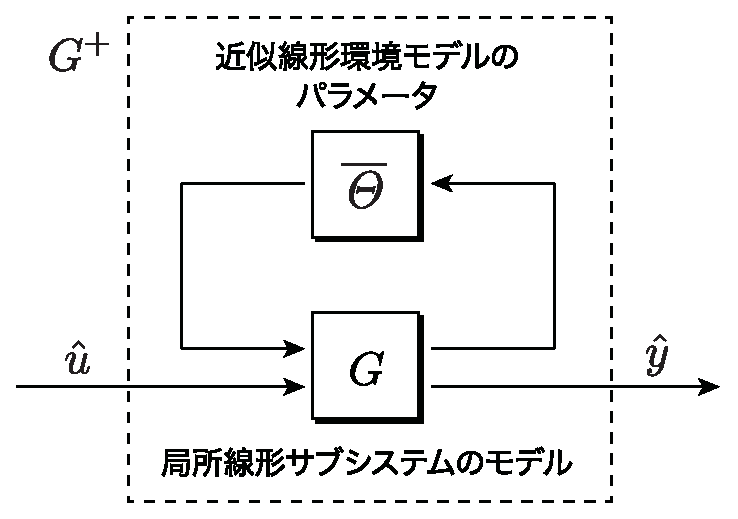
\includegraphics[width = .50\linewidth]{figs/explocalG2}
\medskip
\caption{\textbf{レトロフィットコントローラ設計に用いるモデル}}
\label{fig:explocalG}
\medskip
\end{figure}

\subsection{レトロフィット制御理論に基づく系統安定化装置の設計\advanced}

\smallskip
\subsubsection{レトロフィットコントローラの設計法}

本項では,式\ref{eq:Gbapxst}の近似線形環境パラメータ$\overline{\mathit{\Theta}}$が適当な方法で同定されているものと仮定して,レトロフィットコントローラの設計方法を説明する。
近似線形環境モデルの具体的な構成方法は次項で説明する。

系統安定化装置に対応するレトロフィットコントローラの設計には,システム制御工学における標準的な制御系設計手法を利用することができる。
具体例として,\textbf{線形2次レギュレータ}(LQR:linear-quadratic regulator)の設計手法\cite[5.3節]{fairman1998linear}を式\ref{eq:Gplus}の電力系統モデル$G_+$に適用してみよう。
線形2次レギュレータでは,状態と入力に関するコスト関数
\[
J(\hat{\xi},\hat{u}) :=\int_0^{\infty} \left(
\hat{\xi}^{\sf T}(t) Q \hat{\xi}(t)
+
\hat{u}^{\sf T}(t) R \hat{u}(t)
\right) dt
\]
を最小化する状態フィードバック形式の制御アルゴリズムとして
\begin{align}\label{eq:locKhat}
\hat{u}=\underbrace{-R^{-1}B^{\sf T}P(\overline{\mathit{\Theta}}) }_{\hat{K}(\overline{\mathit{\Theta}}) }
\hat{\xi}
\end{align}
を用いる。
ただし,$Q$は半正定,$R$は正定な行列であり,行列$P(\overline{\mathit{\Theta}})$は\textbf{代数リッカチ方程式}(algebraic Riccati equation)
\[
\left( A+L \overline{\mathit{\Theta}} 
\mathit{\Gamma} \right)^{\sf T} P +
P \left( A+L \overline{\mathit{\Theta}} 
\mathit{\Gamma} \right)
-PB R^{-1} B^{\sf T} P +Q = 0
\]
を満たす正定解である。
このとき,式\ref{eq:locKhat}のゲイン行列$\hat{K}(\overline{\mathit{\Theta}})$を用いて,レトロフィットコントローラは
\begin{align}\label{eq:retroK}
K: \simode{
\dot{\hat{x}} &=  A \hat{x} + L \left\{
v - \overline{\mathit{\Theta}} (w- \mathit{\Gamma} \hat{x}) 
\right\}\\
u &= \hat{K}(\overline{\mathit{\Theta}}) (y - C\hat{x})
}
\end{align}
と構成される。
このレトロフィット制御理論に基づく系統安定化装置は,いかなる行列$\overline{\mathit{\Theta}}$を用いた場合にも
\begin{itemize}
\item 電力系統が定常潮流状態にある場合に入力$u$は0となる
\item 実装の前後で定常潮流状態(平衡点)の安定性は変化しない
\end{itemize}
という特長をもつ
\footnote{
2つ目の項目は,局所コントローラの実装前に漸近安定であった平衡点が,局所コントローラの実装によって不安定な平衡点に変化しないことを意味している。
レトロフィット制御理論では,平衡点の漸近安定性を維持しながら,外乱に対するロバスト性や安定領域の大きさなどを指標とする「安定度の向上」を目的としている。
なお,本手法では,もともと不安定な平衡点を漸近安定化することはできない。
}。
一般に,近似線形環境モデルによる相互作用信号の予測精度が高くなるほど,系統安定度がより大きく向上されることも示されている。
なお,式\ref{eq:locKhat}の制御アルゴリズムは,式\ref{eq:Gplus}の$G_+$を安定化するものであれば,他の制御系設計手法で設計されたものでも構わない。
また,$\hat{K}(\overline{\mathit{\Theta}})$は静的でなくても構わず,動的な制御アルゴリズムとすることもできる\cite{ishizaki2019retrofit}。


\smallskip
\subsubsection{近似線形環境モデルの構成法}

式\ref{eq:Gbapxst}のパラメータ$\overline{\mathit{\Theta}}$を同定する実用的なアプローチは,
式\ref{eq:sigintvw}の信号$w$と$v$の関係を近似線形化により見積もることである。
具体的には,$w$の要素に関する$v$の偏微分は
\begin{align}
\spliteq{
\frac{\partial v }{\partial \delta} &= 
\mat{
- \tfrac{E |\bm{V} |}{ \Xt } \sfcos(\delta -  \angle \bm{V})  \\
- \left( \tfrac{\Xs }{ \Xt }-1 \right)
|\bm{V}| \sfsin (\delta - \angle \bm{V} ) \\
0
}
, \qquad
\frac{\partial v }{\partial \Delta \omega} = \mat{0 \\0\\0} \\
\frac{\partial v }{\partial E} &= 
\mat{
- \tfrac{|\bm{V} |}{ \Xt } \sfsin(\delta -  \angle \bm{V}) \\
0\\
0
}
}
\end{align}
と計算される。
したがって,注目する発電機の内部状態と発電機母線の電圧フェーザが定常潮流状態の近傍にあることを仮定すると
\begin{align}\label{eq:basenvm}
\overline{\mathit{\Theta}}_{0} =
\mat{
- \tfrac{E^{\star} |\bm{V}^{\star} |}{ \Xt } \sfcos(\delta^{\star} -  \angle \bm{V}^{\star}) &
0   & 
- \tfrac{|\bm{V}^{\star} |}{ \Xt } \sfsin(\delta^{\star} -  \angle \bm{V}^{\star})
\\
- \left( \tfrac{ \Xs }{ \Xt }-1 \right) 
|\bm{V}^{\star}| \sfsin (\delta^{\star} - \angle \bm{V}^{\star} ) 
& 0 
& 0 
\\
0 & 0 &0
}
\end{align}
が得られる。
ここで,発電機の内部状態の定常値$(\delta^{\star},E^{\star})$と母線電圧フェーザの定常値$(|\bm{V}^{\star}|,\angle \bm{V}^{\star})$は,式\ref{eq:Gbapxst}の$(v^{\star},w^{\star})$と同じ定常潮流状態における値である。
式\ref{eq:basenvm}の行列$\overline{\mathit{\Theta}}_{0}$により,発電機の内部状態がそれ自身に与える局所的なフィードバック構造をモデル化することができる。
なお,通常の電力系統は定常潮流状態の近傍で運転されているため,モデルの構築に必要となる定常値は計測データに基づいて同定することができる。


つぎに,自動発電制御を介して信号$w$が信号$v$に与える間接的な影響を見積もることを考えよう。
自動発電制御の入力$P_{\rm mech}$に関する$v$の偏微分は
\[
\frac{\partial v}{\partial P_{\rm mech}}
=
\mat{
1\\0\\0
}
\]
となる。
式(\ref{eq:agccon})のブロードキャスト型PIコントローラが自動発電制御として組み込まれている場合には,$\Delta \omega$の積分が$\delta$に相当することに注意すると
\[
\frac{\partial P_{\rm mech}}{\partial \delta} = -  \alpha \beta k_{\rm I}
,\qquad
\frac{\partial P_{\rm mech}}{\partial \Delta \omega}= - \alpha \beta k_{\rm P}
,\qquad
\frac{\partial P_{\rm mech}}{\partial E}= 0
\]
がわかる。
したがって,微分の連鎖律により,ブロードキャスト型PIコントローラを介して信号$w$が信号$v$に与える影響は
\begin{align}
\overline{\mathit{\Theta}}_{\rm agc}:=
-  \alpha \beta \mat{
 k_{\rm I} &  k_{\rm P} & 0\\
0 & 0 & 0\\
0 & 0 & 0
}
\end{align}
によりモデル化できる。
ただし,このパラメータを得るためには,自動発電制御のコントローラゲインの値を適当な方法で取得する必要がある。

同様に,母線電圧フェーザ$\bm{V}$を介して信号$w$が信号$v$に与える間接的な影響を見積もることを考える。
電圧フェーザ変数$(|\bm{V}|,\angle \bm{V})$に関する$v$の偏微分は
\begin{align}
\spliteq{
\frac{\partial v }{\partial |\bm{V}|} &= 
\mat{
-\tfrac{E }{ \Xt } \sfsin(\delta -  \angle \bm{V})  \\
\left( \tfrac{ \Xs }{ \Xt }-1 \right)
\sfcos (\delta - \angle \bm{V} ) \\
1
}
\\
\frac{\partial v }{\partial \angle \bm{V}} &= 
\mat{
\tfrac{E|\bm{V} |}{ \Xt } \sfcos(\delta -  \angle \bm{V}) \\
\left( \tfrac{ \Xs }{ \Xt }-1 \right)
|\bm{V}|\sfsin (\delta - \angle \bm{V} ) \\
0
}
}
\end{align}
と計算できる。
一方で,母線電圧フェーザは,\ref{sec:allgen}節で解析されているように,接続されている発電機の内部状態だけでなく,他のすべての発電機の内部状態にも依存して変化する。
具体的には,注目する発電機を除くすべての発電機の内部状態を並べたベクトルを$\overline{\delta}$,$\overline{E}$と表すとき,
$\tfrac{\partial |\bm{V}| }{\partial \delta}$,
$\tfrac{\partial \angle \bm{V} }{\partial \delta}$,
$\tfrac{\partial |\bm{V}| }{\partial E}$,
$\tfrac{\partial \angle \bm{V} }{\partial E}$の4つの偏微分は,すべての発電機の内部状態をまとめた
\[
z_{\mathds G}:=(\delta,\overline{\delta},E,\overline{E})
\]
に依存する関数となる。
一般の電力系統モデルに対して,これらの偏導関数を解析的に求めることは容易ではないが,定常潮流状態の近傍において
\begin{align}\label{eq:thetaV}
\theta_{\bm{V}}
:=
\mat{
\tfrac{\partial |\bm{V}| }{\partial \delta}(z_{\mathds G}^{\star}) &
0 &
\tfrac{\partial |\bm{V}| }{\partial E}(z_{\mathds G}^{\star}) \\
\tfrac{\partial \angle \bm{V} }{\partial \delta}(z_{\mathds G}^{\star}) &
0 &
\tfrac{\partial \angle \bm{V} }{\partial E}(z_{\mathds G}^{\star})
}
\end{align}
の数値を計測データなどを用いて同定することができれば,母線電圧フェーザ$\bm{V}$を介して信号$w$が信号$v$に与える影響を
\begin{align}\label{eq:ThetaV}
\overline{\mathit{\Theta}}_{\bm{V}}:=
\mat{
-\tfrac{E^{\star} }{ \Xt } \sfsin(\delta^{\star} -  \angle \bm{V}^{\star}) 
 &
\tfrac{E^{\star}|\bm{V}^{\star} |}{ \Xt } \sfcos(\delta^{\star} -  \angle \bm{V}^{\star}) 
\\
\left( \tfrac{ \Xs }{ \Xt }-1 \right)
\sfcos (\delta^{\star} - \angle \bm{V}^{\star} )  
&
\left( \tfrac{ \Xs }{ \Xt }-1 \right)
|\bm{V}^{\star}|\sfsin (\delta^{\star} - \angle \bm{V}^{\star} )
\\
1 & 0
}
\hat{\theta}_{\bm{V}}
\end{align}
によりモデル化できる
\footnote{
電力系統は常に安定に運用されている必要があるため,式\ref{eq:ThetaV}の$\theta_{\bm{V}}$は運用しながら計測されたデータを
用いて同定する必要がある。
システム制御工学では,動作しているフィードバック系内のサブシステムの同定は,\textbf{閉ループ同定}(closed-loop identification)と呼ばれる\cite{ljung1998system}。
閉ループ同定は,同定対象の入力を自由に励振することが一般にできないため,入力の励振が可能な場合の同定よりも難しいことが多い。
}。
ただし,式\ref{eq:thetaV}の$z_{\mathds G}^{\star}$は$z_{\mathds G}$の定常値を表しており,
第2列の0要素は$\tfrac{\partial |\bm{V}| }{\partial \Delta \omega}$,$\tfrac{\partial \angle \bm{V} }{\partial \Delta \omega}$に対応している。
また,式\ref{eq:ThetaV}の$\hat{\theta}_{\bm{V}}$は$\theta_{\bm{V}}$の同定された値を表している。
以上の近似線形化による見積もりを同時に用いる場合には,式\ref{eq:Gbapxst}のモデルパラメータは
\[
\overline{\mathit{\Theta}}=
\overline{\mathit{\Theta}}_{0}+
\overline{\mathit{\Theta}}_{\rm agc}+
\overline{\mathit{\Theta}}_{\bm{V}}
\]
と構成される。
なお,前項で説明されたように,式\ref{eq:retroK}の系統安定化装置は,いかなる行列$\overline{\mathit{\Theta}}$に対しても定常潮流状態の安定性を変化させない。
一方で,近似線形環境モデルによる相互作用信号の予測精度を適切に維持するためには,$\overline{\mathit{\Theta}}$を潮流状態に応じて適当な頻度で更新することが望ましい。


\newpage
%\printindex
%
%
\end{document}